\documentclass{article}

\usepackage[preprint]{neurips_2026}
\usepackage[utf8]{inputenc}
\usepackage[T1]{fontenc}
\usepackage{microtype}
\usepackage{graphicx}
\usepackage{booktabs}
\usepackage{tabularx}
\usepackage{array}
\usepackage{multirow}
\usepackage{xcolor}
\usepackage{tikz}
\usepackage{caption}
\usepackage{subcaption}
\usepackage{enumitem}
\usepackage{amsmath}
\usepackage{url}
\usepackage{hyperref}
\usetikzlibrary{arrows.meta,positioning,fit}

\graphicspath{{figures/}}
\newcommand{\ra}{ResearchArena}
\newcommand{\sar}{SAR}
\newcommand{\pr}{PR}
\newcommand{\agent}[1]{\textsc{#1}}
\newcommand{\yes}{Yes}
\newcommand{\no}{No}
\newcommand{\maybe}{Partial}

\title{ResearchArena: Process-Grounded Evaluation of End-to-End Research by CLI Agents}

\author{Anonymous Authors}

\begin{document}

\maketitle

\begin{abstract}
Auto-research is not just paper generation. A research agent must form an idea, implement and run experiments, interpret outputs, cite prior work, and write a manuscript that remains faithful to the artifacts produced by the process. We introduce \ra, a benchmark and empirical study of off-the-shelf command-line agents performing an end-to-end research pipeline under a minimal scaffold. \ra\ contains 117 agent-generated papers from Claude Code, Codex, and Kimi Code across 13 computer-science domains, together with code, configurations, execution logs, result files, reviews, and metadata. We also introduce artifact-grounded peer review, an evaluation protocol in which reviewers inspect the final paper together with the code, logs, result artifacts, and references. This protocol evaluates paper-artifact faithfulness rather than only paper plausibility. Across the study, current CLI agents often complete research-like artifacts, but completion does not imply validity: experimental rigor, scientific significance, reference integrity, and paper-artifact faithfulness remain the dominant bottlenecks. PDF-only review assigns substantially higher apparent quality than artifact-grounded review, especially for papers whose reported settings or results cannot be reconstructed from the released artifacts.
\end{abstract}

\section{Introduction}

Auto-research is not just paper generation. A system that produces a plausible PDF has not necessarily conducted a valid research process: it may have proposed a weak question, implemented a different method from the one described, run only a subset of the claimed experiments, copied numbers incorrectly, or cited nonexistent prior work. For end-to-end research agents, the central evaluation problem is therefore not only whether the final manuscript looks convincing, but whether the manuscript is faithful to the research that was actually conducted.

This distinction is increasingly important as general-purpose command-line agents become capable of operating full software environments. CLI agents can read papers, edit code, run experiments, inspect logs, revise drafts, and assemble final PDFs. These abilities make them natural substrates for automated research pipelines, but they also create new failure modes. A final paper can look coherent while its code fails to implement the method, its logs show incomplete runs, or its reported numbers diverge from stored results.

We introduce \ra, a benchmark and study of off-the-shelf CLI agents conducting an end-to-end research pipeline with minimal scaffolding. The benchmark covers three widely used CLI agents--Claude Code, Codex, and Kimi Code--across 13 computer-science domains, including 5 CPU-only and 8 GPU domains. Each agent generates 39 papers, for 117 papers total. For every run, \ra\ records the final paper, code, configurations, execution logs, result artifacts, reviews, and metadata.

We also introduce artifact-grounded peer review. In contrast to PDF-only review, artifact-grounded peer review gives reviewers access to the paper and its process artifacts: code, logs, result files, and references. The goal is not to claim that one automatic reviewer is universally better than another. Rather, PDF-only and artifact-grounded review evaluate different targets. PDF-only review asks whether the final manuscript looks convincing. Artifact-grounded peer review asks whether the paper is faithful to the research process and evidence that produced it.

\paragraph{Contributions.}
First, we present \ra, a large-scale empirical evaluation of off-the-shelf CLI agents conducting end-to-end research-like workflows under a minimal scaffold. The dataset contains 117 generated papers and 351 artifact-grounded peer reviews across 13 CS domains. Second, we define and instantiate artifact-grounded peer review as a process-grounded evaluation protocol for auto-research. The protocol reveals unsupported results, setting mismatches, incomplete experiments, hallucinated references, and weak baselines that are often invisible from the PDF alone.

\paragraph{Summary of findings.}
Current CLI agents can often complete the research loop, but completion does not imply validity. Under Stanford Agentic Reviewer (\sar), a PDF-only reviewer, Claude Code scores 5.45, Codex 4.93, and Kimi Code 4.24 on a 0--10 ICLR-style scale; Claude Code sits near the weighted mean of a sampled ICLR 2025 submission set. Under artifact-grounded peer review (\pr), scores fall to 4.59, 4.51, and 3.38, respectively. The gap is not a contradiction: it reflects a change in evaluation target from apparent paper quality to paper-artifact faithfulness. Across agents, experimental rigor and significance are the dominant bottlenecks. Codex is the strongest on integrity-related dimensions, Claude Code is strongest on novelty and significance, and Kimi Code has the highest mismatch and fake-reference rates. Scaling Codex GPU runs from RTX A6000 to H100 changes \pr\ from about 4.50 to 4.26, suggesting that additional compute alone does not reliably improve auto-research quality.

\section{Related Work}

\paragraph{Automated research systems.}
Recent systems aim to automate parts of the scientific workflow, including ideation, experiment execution, manuscript writing, and self-improvement. Examples include The AI Scientist \citep{lu2024ai}, Agent Laboratory \citep{schmidgall2025agentlaboratory}, and FARS \citep{analemma2025fars}. These systems demonstrate that LLM-based agents can assemble research-like artifacts, but they also raise evaluation questions that are not captured by final-paper appearance alone. \ra\ differs by focusing on off-the-shelf CLI agents under minimal scaffolding and by retaining the full process trace needed for artifact-grounded auditing.

\paragraph{CLI agents and agentic coding systems.}
General-purpose coding agents such as Claude Code, Codex, and Kimi Code operate directly in software repositories and shell environments \citep{anthropic2026opus,anthropic2026claudecode,openai2026codex,moonshot2026kimi,moonshot2026kimicode}. Their ability to edit files, run experiments, and debug failures makes them suitable for end-to-end research pipelines. Coding benchmarks such as SWE-bench \citep{jimenez2024swebench} evaluate issue resolution in real repositories, while \ra\ evaluates a broader research loop that includes problem framing, empirical design, paper writing, and review.

\paragraph{LLM-as-reviewer and paper-review agents.}
LLM-based reviewing systems estimate paper quality, generate review text, or calibrate scores against venue decisions. Stanford Agentic Reviewer provides an ICLR-style score from a submitted manuscript \citep{stanford2026sar}. Related work studies LLM reviewing behavior, reviewer calibration, and biases in automatic evaluation \citep{liang2024llmjudge,zhou2024reviewer2}. \ra\ uses \sar\ as a PDF-only comparison point, but its methodological focus is artifact-grounded review: reviewers inspect the paper together with code, logs, result files, and references.

\paragraph{Reproducibility, artifact evaluation, and scientific integrity.}
Artifact evaluation practices in systems and machine-learning venues emphasize reproducibility, code availability, and the relationship between claims and executable artifacts \citep{pineau2021improving,collberg2016repeatability,acm2020badging}. These practices motivate our evaluation target. A generated paper may be clear and plausible while failing to match its own code or logs. \ra\ adapts the spirit of artifact evaluation to auto-research by making paper-artifact faithfulness a first-class evaluation criterion.

\section{ResearchArena Benchmark}

\ra\ evaluates whether off-the-shelf CLI agents can complete an end-to-end research pipeline under a minimal scaffold. The scaffold provides domain seeds, resource limits, stage prompts, and review instructions, but it does not provide a hand-designed research method, curated experimental codebase, or fixed paper template beyond normal conference-style expectations.

\begin{figure}[t]
\centering
\resizebox{\linewidth}{!}{%
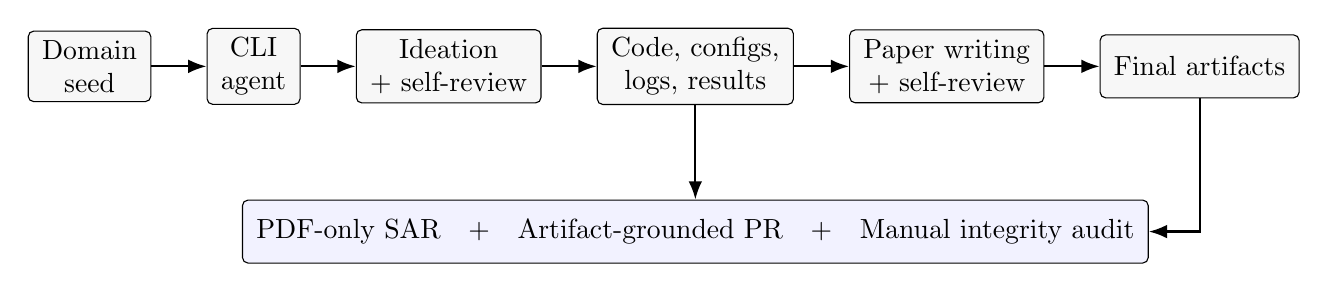
\begin{tikzpicture}[
  node distance=7mm,
  box/.style={draw, rounded corners=2pt, align=center, minimum height=8mm, inner xsep=5pt, fill=gray!6},
  wide/.style={draw, rounded corners=2pt, align=center, minimum height=8mm, inner xsep=5pt, fill=blue!5},
  arrow/.style={-Latex, thick}
]
\node[box] (seed) {Domain\\seed};
\node[box, right=of seed] (agent) {CLI\\agent};
\node[box, right=of agent] (idea) {Ideation\\+ self-review};
\node[box, right=of idea] (exp) {Code, configs,\\logs, results};
\node[box, right=of exp] (paper) {Paper writing\\+ self-review};
\node[box, right=of paper] (final) {Final artifacts};
\node[wide, below=12mm of exp] (eval) {PDF-only \sar\quad+\quad Artifact-grounded \pr\quad+\quad Manual integrity audit};
\draw[arrow] (seed) -- (agent);
\draw[arrow] (agent) -- (idea);
\draw[arrow] (idea) -- (exp);
\draw[arrow] (exp) -- (paper);
\draw[arrow] (paper) -- (final);
\draw[arrow] (final.south) |- (eval.east);
\draw[arrow] (exp.south) -- (eval.north);
\end{tikzpicture}
}
\caption{\ra\ workflow. Agents proceed from a domain seed through ideation, experiments, paper writing, self-review, and final evaluation. Artifact-grounded review uses the paper together with code, logs, results, and references.}
\label{fig:workflow}
\end{figure}

\begin{table}[t]
\centering
\small
\begin{tabularx}{\linewidth}{l l c c c c}
\toprule
Agent & Model & CPU seeds & GPU seeds & Trials/seed & Papers \\
\midrule
Claude Code & Opus 4.6 & 5 & 8 & 3 & 39 \\
Codex & GPT-5.4 & 5 & 8 & 3 & 39 \\
Kimi Code & K2.5 & 5 & 8 & 3 & 39 \\
\midrule
Total & -- & 5 & 8 & 3 & 117 \\
\bottomrule
\end{tabularx}
\caption{Benchmark setup. Each agent generates one paper for each trial in each domain seed. CPU seeds are causal learning, compiler optimization, data integration and cleaning, operating-system design, and probabilistic methods. GPU seeds are AI for biology, computer vision, datasets and benchmarks, generative models, interpretability of learned representations, NLP, privacy in ML, and supervised representation learning.}
\label{tab:setup}
\end{table}

\paragraph{Agents and domains.}
Table~\ref{tab:setup} summarizes the study design. We evaluate Claude Code, Codex, and Kimi Code. Each agent produces 39 papers: three trials for each of 13 domain seeds. The CPU-only domains emphasize algorithmic, systems, and data-management tasks that can be run without accelerators. The GPU domains emphasize modern ML areas where training, fine-tuning, or model evaluation is common.

\paragraph{Hardware.}
Main experiments use either CPU-only resources or one NVIDIA RTX A6000 GPU with 48GB memory. Each agent receives 4 CPU cores and 60GB RAM. We additionally run a Codex GPU scaling experiment on NVIDIA H100 GPUs with 80GB memory while holding other settings fixed.

\paragraph{Pipeline.}
Each run follows the same high-level stages. During ideation, the agent proposes a research question and experiment plan, with up to three rounds of self-review and revision. During experimentation, the agent writes and executes code, records logs, and stores result artifacts, again with self-review. During paper writing, the agent drafts the manuscript and revises it through self-review. Finally, the paper is evaluated by \sar\ and by artifact-grounded peer review.

\paragraph{Collected artifacts.}
For each generated paper, \ra\ retains the final PDF or source manuscript, experiment code, configuration files, execution logs, result files such as JSON or CSV outputs, generated figures, self-reviews, peer reviews, Stanford Agentic Reviewer output, and metadata. The retained artifacts make it possible to evaluate not only what the paper says, but whether the evidence in the workspace supports it.

\section{Artifact-Grounded Peer Review}

\ra\ uses two complementary review modes. \textbf{PDF-only review} evaluates the final manuscript as a standalone paper. In our study, \sar\ provides this view: it receives the paper and returns an ICLR-style score. \textbf{Artifact-grounded review} evaluates the paper together with the code, execution logs, result artifacts, and references. This mode evaluates paper-artifact faithfulness, not just paper plausibility.

\begin{table}[t]
\centering
\small
\begin{tabularx}{\linewidth}{p{0.28\linewidth} X X}
\toprule
Evaluation target & PDF-only \sar & Artifact-grounded \pr \\
\midrule
Inputs available & Final manuscript & Manuscript plus code, configs, logs, result files, figures, and references \\
Can inspect code? & \no & \yes \\
Can inspect logs? & \no & \yes \\
Can verify result files? & \no & \yes \\
Can detect setting mismatch? & Usually no & Yes, when settings are encoded in code, configs, or logs \\
Can detect fake references? & Partly from bibliography text & Yes, with explicit reference checks \\
Main failure mode & Rewards plausible but unsupported papers & Depends on reviewer skill and can still miss subtle defects \\
\bottomrule
\end{tabularx}
\caption{Evaluation target comparison. PDF-only review and artifact-grounded peer review answer different questions. The latter audits the relationship between claims and process artifacts.}
\label{tab:target-comparison}
\end{table}

\paragraph{Rubric.}
Every paper is reviewed by all three CLI agents, producing 351 peer reviews in total. Reviewers score nine dimensions on a 0--10 ICLR-style scale: novelty, soundness, significance, clarity, reproducibility, experimental rigor, references, reference integrity, and results integrity. The overall \pr\ score is the mean of the reviewers' overall scores. We report both aggregate scores and dimension-level patterns.

\paragraph{Reviewer aggregation.}
The use of all three agents as reviewers is deliberate. Reviewer severity varies substantially: Codex is the strictest reviewer, Kimi Code is the most lenient, and Claude Code lies between them. Multi-reviewer aggregation reduces dependence on any single reviewer's calibration. It does not eliminate bias, but it exposes severity differences that would be hidden under a single-reviewer protocol.

\paragraph{Manual integrity audit.}
In addition to automatic peer review, we manually annotate every generated paper for four integrity categories: result mismatch only, setting mismatch only, both result and setting mismatch, and fake references. A result mismatch means reported numbers do not match stored outputs or logs. A setting mismatch means the paper describes a method, dataset, baseline, hyperparameter, scale, or execution setting that differs from the artifact. The ``both'' category records papers exhibiting both mismatch types. Fake references include nonexistent citations, fabricated metadata, or references that cannot be verified as stated.

\paragraph{Conceptual decomposition.}
The results suggest a useful decomposition for evaluating auto-research systems: apparent paper quality, artifact faithfulness, and process reliability. Apparent paper quality captures whether the manuscript reads like a competent submission. Artifact faithfulness captures whether the manuscript is supported by code, logs, and result files. Process reliability captures whether the agent consistently designs, executes, records, and interprets experiments without drift. A system can score well on the first component while failing the latter two; artifact-grounded review is designed to make those failures visible.

\section{Main Results}

We organize the empirical findings around six research questions.

\paragraph{RQ1: Can CLI agents complete end-to-end research under minimal scaffolding?}
Yes, in the limited sense of producing complete research-like artifacts. All three agents generate papers, code, logs, results, and reviews across the full domain set, yielding 117 papers. However, completion should not be confused with validity. Many papers contain incomplete baselines, unsupported claims, setting mismatches, or results that cannot be reconstructed from artifacts.

\begin{table}[t]
\centering
\small
\begin{tabular}{lrrrrrr}
\toprule
System & $n$ & \sar\ mean & \sar\ std. & Min & Max & $\geq 5.0$ \\
\midrule
Claude Code & 39 & 5.45 & 0.70 & 3.1 & 6.3 & 82\% \\
FARS & 102 & 5.06 & 0.62 & 3.0 & 6.3 & 76\% \\
Codex & 39 & 4.93 & 0.85 & 2.7 & 6.3 & 64\% \\
Kimi Code & 39 & 4.24 & 0.84 & 2.0 & 5.3 & 26\% \\
\bottomrule
\end{tabular}
\caption{PDF-only \sar\ comparison. We treat FARS as a secondary external reference point rather than as the central comparison target.}
\label{tab:sar-system}
\end{table}

\begin{figure}[t]
\centering
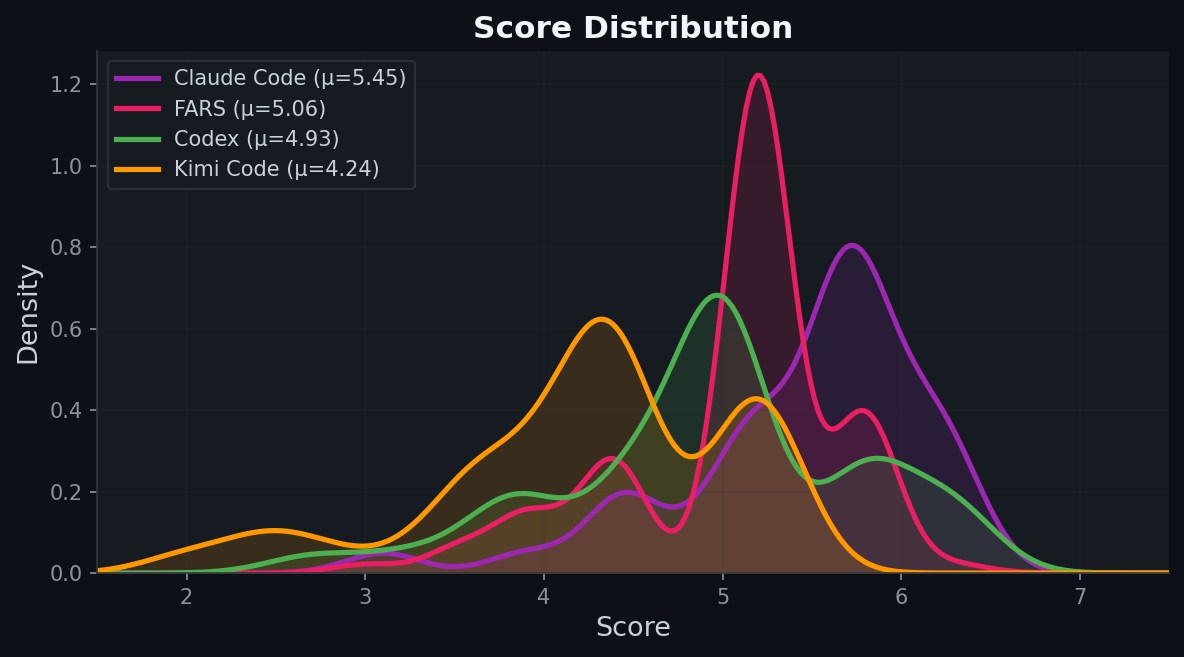
\includegraphics[width=0.86\linewidth]{sar_score_distributions.png}
\caption{\sar\ score distributions. PDF-only review assigns many generated papers scores near the middle of the ICLR scale, with Claude Code highest among the three CLI agents.}
\label{fig:sar-dist}
\end{figure}

\paragraph{RQ2: How do \sar\ and \pr\ differ?}
Table~\ref{tab:sar-system} and Figure~\ref{fig:sar-dist} show the PDF-only \sar\ view. Claude Code scores 5.45, Codex 4.93, and Kimi Code 4.24; FARS reports 5.06 on 102 papers. A human-calibration sample gives ICLR accepted papers a \sar\ mean of 5.59, a weighted ICLR mean of 5.42, and rejected papers 5.34. Human-annotated \sar\ accept rates are more separated: ICLR accepted 76.0\%, ICLR rejected 52.0\%, Claude Code 41.0\%, FARS 21.6\%, Codex 12.8\%, and Kimi Code 5.1\%.

Artifact-grounded \pr\ is stricter: Claude Code scores 4.59, Codex 4.51, and Kimi Code 3.38. The important point is not that \pr\ is a better scalar judge in all settings, but that it evaluates a different object. \sar\ evaluates the final PDF. \pr\ evaluates whether the PDF is supported by the research artifacts.

\begin{figure}[t]
\centering
\begin{subfigure}{0.48\linewidth}
\centering

\includegraphics[width=\linewidth]{pr_score_distributions.png}
\caption{\pr\ distributions}
\label{fig:pr-dist}
\end{subfigure}
\hfill
\begin{subfigure}{0.48\linewidth}
\centering
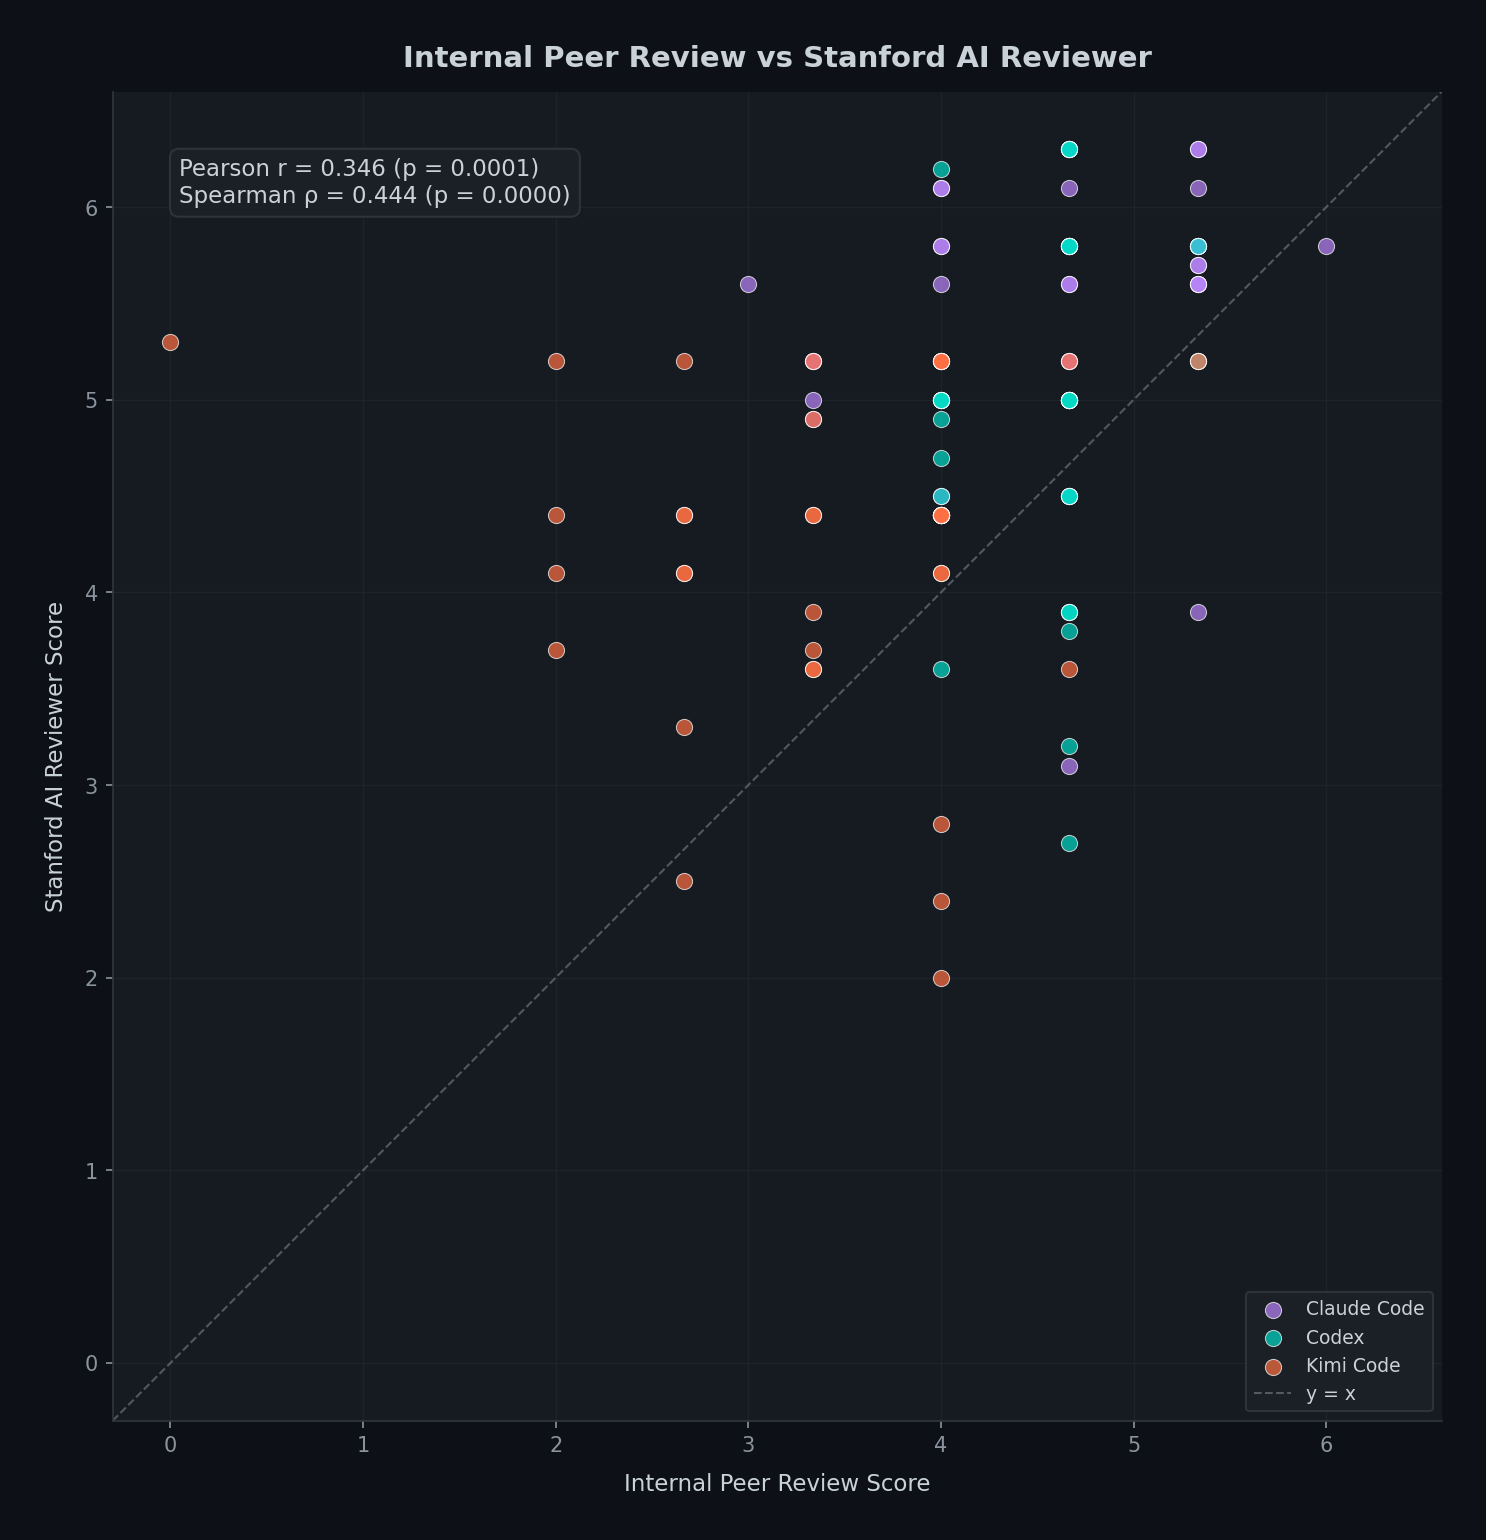
\includegraphics[width=\linewidth]{internal_vs_stanford_scatter.png}
\caption{\sar\ versus \pr}
\label{fig:sar-pr-scatter}
\end{subfigure}
\caption{Artifact-grounded review shifts the evaluation target from paper plausibility to paper-artifact faithfulness. Scores fall most when artifacts reveal unsupported results, setting mismatches, or incomplete experiments.}
\label{fig:pr-and-scatter}
\end{figure}

\paragraph{RQ3: What are the dominant bottlenecks?}
Across agents, experimental rigor and significance are the recurring weaknesses. Figure~\ref{fig:dimensions} shows that Codex leads on reproducibility, reference integrity, and results integrity, while Claude Code leads on novelty and significance. Kimi Code trails on most dimensions. The lowest dimensions are not simply novelty: the agents frequently produce plausible ideas but fail to validate them with strong baselines, adequate scale, consistent protocols, or faithful reporting.

\begin{figure}[t]
\centering
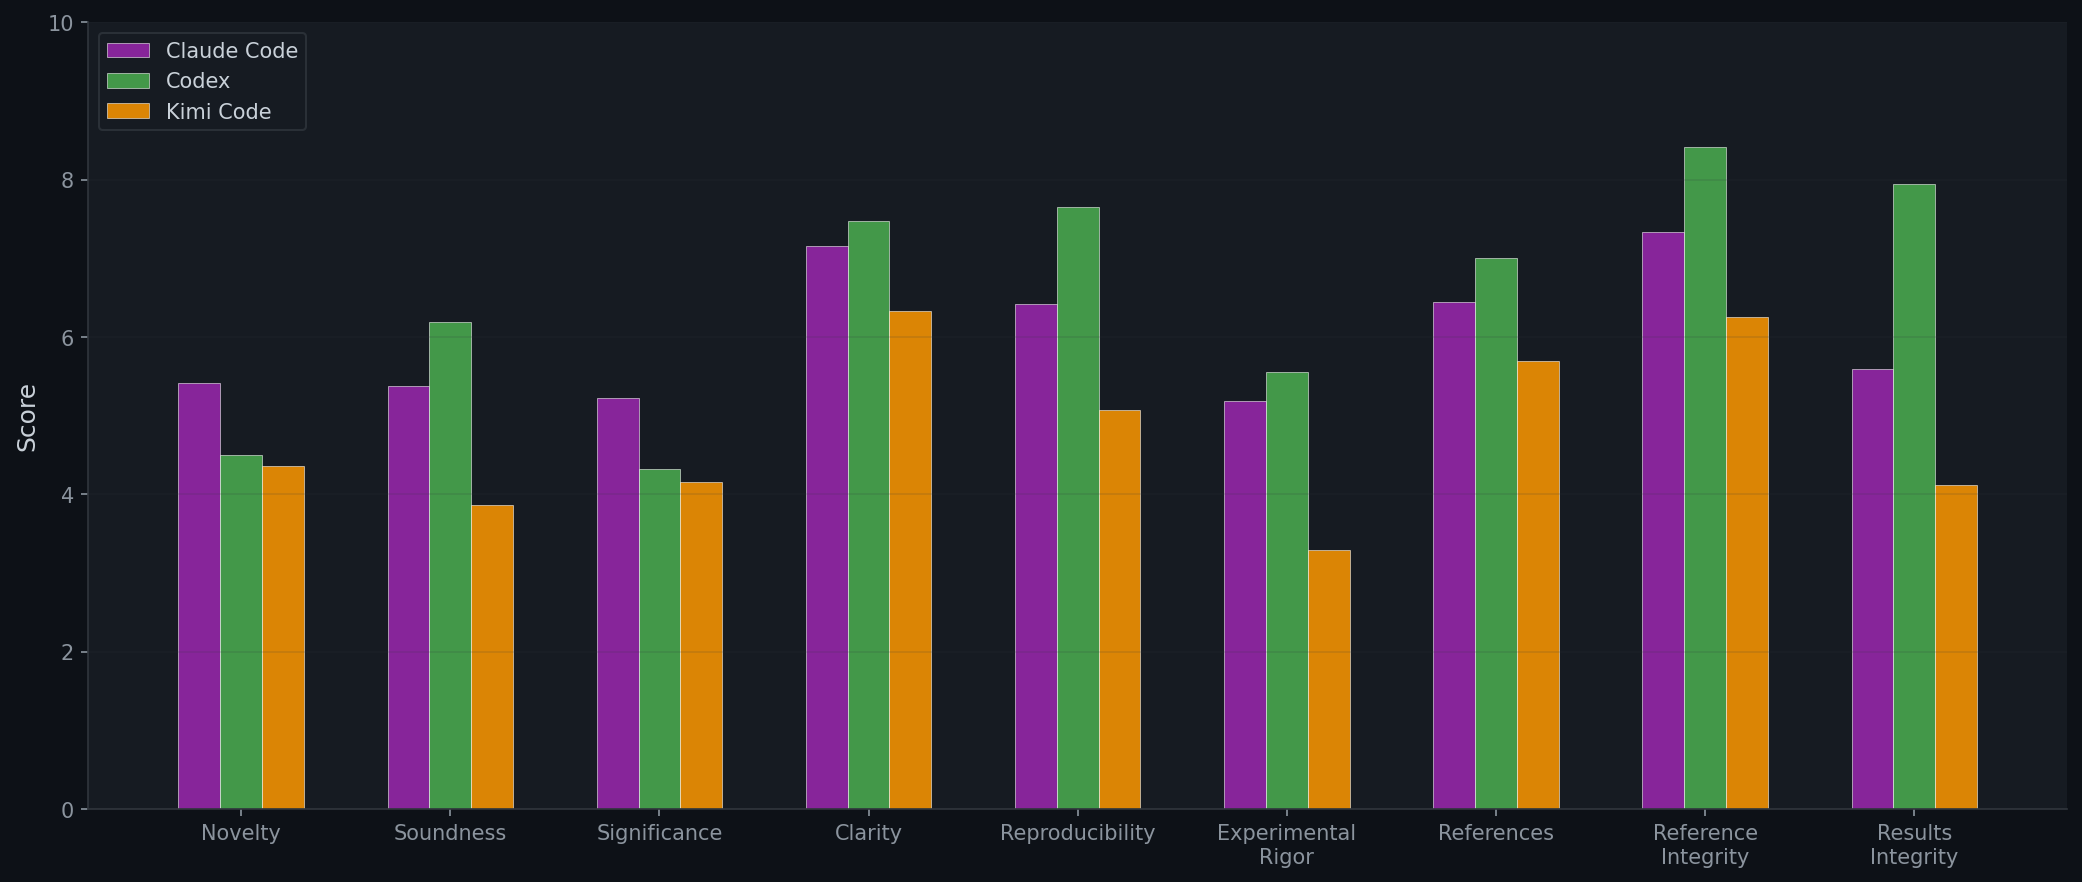
\includegraphics[width=0.9\linewidth]{comparison_3way_dimensions.png}
\caption{Per-dimension \pr\ scores. Codex is strongest on integrity-oriented dimensions, Claude Code is strongest on novelty and significance, and experimental rigor remains the dominant bottleneck.}
\label{fig:dimensions}
\end{figure}

\begin{table}[t]
\centering
\small
\begin{tabular}{lrrr}
\toprule
Integrity category & Claude Code & Codex & Kimi Code \\
\midrule
Results mismatch only & 6/39 & 2/39 & 4/39 \\
Setting mismatch only & 10/39 & 1/39 & 5/39 \\
Both results and setting mismatch & 12/39 & 2/39 & 30/39 \\
Fake reference & 14/39 & 3/39 & 28/39 \\
\bottomrule
\end{tabular}
\caption{Manual integrity audit. Artifact inspection reveals paper-artifact mismatches and fake references that are often not visible from the PDF alone.}
\label{tab:integrity}
\end{table}

\paragraph{RQ4: Do agents exhibit distinct research personas?}
The agents show stable differences in research style (Table~\ref{tab:personas}). Claude Code behaves like a full-stack researcher: it writes the longest papers, uses more figures and tables, and balances empirical studies with novel methods. Codex behaves like an empirical scientist: 87\% of its papers are controlled empirical studies, with high integrity but lower novelty. Kimi Code behaves like a system builder: it proposes acronym-heavy named methods, but has high mismatch and fake-reference rates.

\begin{table}[t]
\centering
\small
\begin{tabularx}{\linewidth}{lrrrrX}
\toprule
Agent & Novel method & Benchmark & Extension & Empirical & Summary \\
\midrule
Claude Code & 33\% & 8\% & 13\% & 46\% & Balanced, broad, longest papers, more figures and tables \\
Codex & 8\% & 0\% & 5\% & 87\% & Controlled empirical studies, highest integrity, lower novelty \\
Kimi Code & 79\% & 10\% & 0\% & 10\% & Named methods and acronyms, high mismatch and fake-reference rates \\
\bottomrule
\end{tabularx}
\caption{Research type distribution and qualitative personas. Style explains part of the score profile: Codex is reliable but narrow, Claude Code is broader, and Kimi Code often overproduces method framing relative to evidence.}
\label{tab:personas}
\end{table}

\paragraph{RQ5: Does more compute improve research quality?}
More compute does not reliably improve quality in this study. Figure~\ref{fig:domains-time} shows CPU/GPU differences and per-domain variation. Under \pr, all agents score higher on CPU tasks than GPU tasks, while \sar\ sometimes shows the opposite trend. This suggests that GPU domains can yield more polished-looking papers while also being harder to execute faithfully.

\begin{figure}[t]
\centering
\begin{subfigure}{0.48\linewidth}
\centering

\includegraphics[width=\linewidth]{pr_per_domain_breakdown.png}
\caption{Per-domain \pr}
\end{subfigure}
\hfill
\begin{subfigure}{0.48\linewidth}
\centering
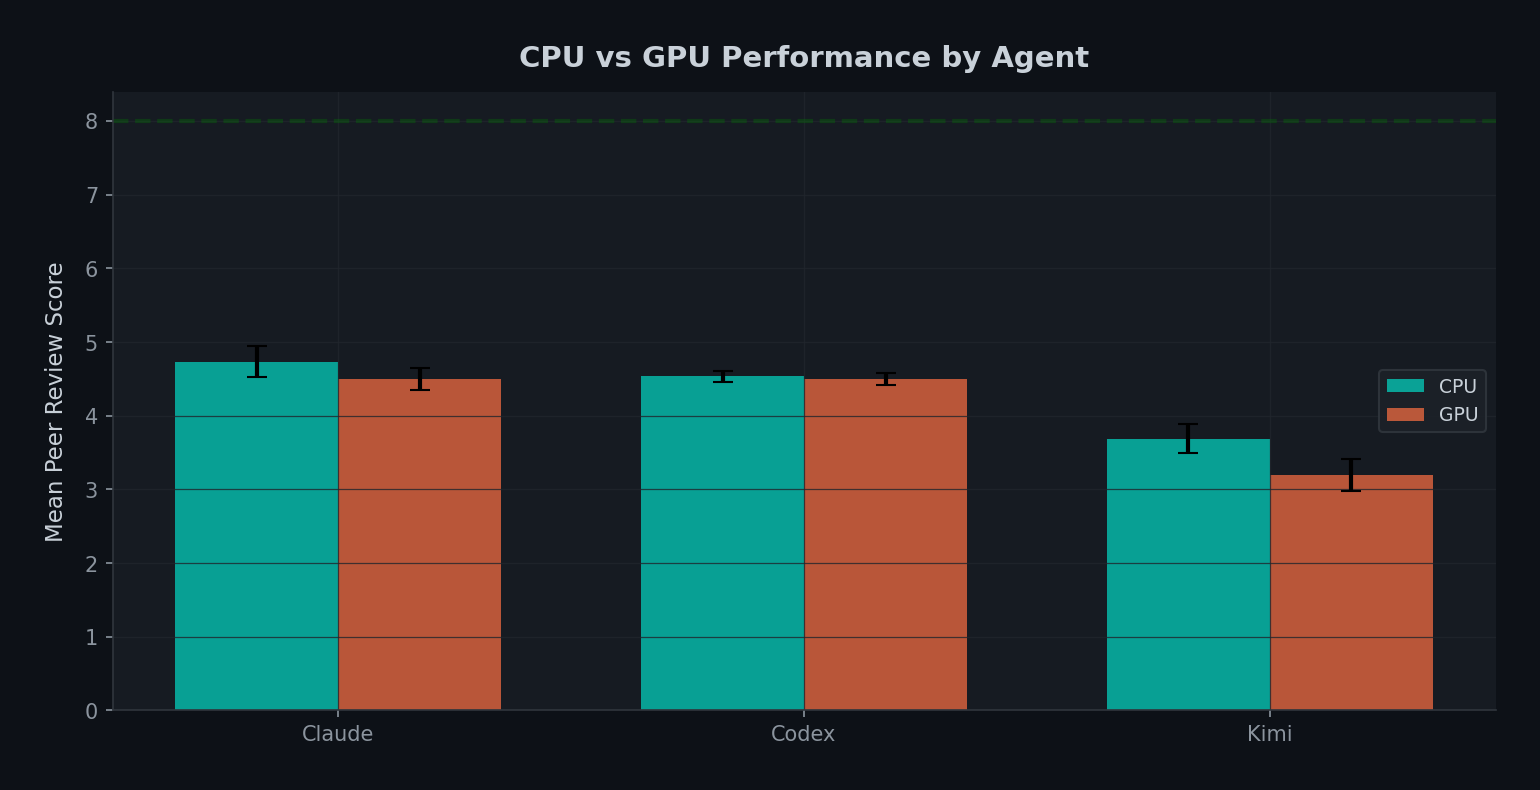
\includegraphics[width=\linewidth]{comparison_3way_cpu_gpu_gap.png}
\caption{CPU/GPU gap}
\end{subfigure}
\caption{Domain and hardware patterns. Artifact-grounded review exposes a CPU/GPU divergence: visually polished GPU-domain papers often suffer from harder execution and verification conditions.}
\label{fig:domains-time}
\end{figure}

\begin{table}[t]
\centering
\small
\begin{tabular}{lrrr}
\toprule
GPU domain seed & Codex H100 \pr & Codex A6000 \pr & Difference \\
\midrule
AI for Biology & 4.89 & 4.67 & +0.22 \\
Interpretability of Learned Repr. & 4.78 & 4.67 & +0.11 \\
Computer Vision & 4.33 & 4.33 & +0.00 \\
Natural Language Processing & 4.22 & 4.33 & -0.11 \\
Privacy in ML & 4.22 & 4.00 & +0.22 \\
Supervised Repr. Learning & 4.22 & 4.67 & -0.45 \\
Generative Models & 3.78 & 4.33 & -0.55 \\
Datasets and Benchmarks & 3.67 & 4.67 & -1.00 \\
\midrule
Average & 4.26 & 4.50 & -0.24 \\
\bottomrule
\end{tabular}
\caption{H100 scaling experiment for Codex GPU runs. Moving from A6000 to H100 does not improve aggregate \pr; the average change is about -0.25 points. This suggests, but does not prove, that compute is not the primary bottleneck.}
\label{tab:h100}
\end{table}

\paragraph{RQ6: What failures are revealed by artifact inspection?}
Table~\ref{tab:integrity} summarizes manual integrity failures. Kimi Code has the highest mismatch rates: 30/39 papers exhibit both result and setting mismatch, and 28/39 contain fake references. Claude Code is intermediate, while Codex has the lowest mismatch and fake-reference rates. These defects are precisely the type that can survive PDF-only review. A paper can present a consistent story while its artifacts show a smaller benchmark sweep, a different evaluation protocol, a missing baseline, or numbers copied from the wrong file.

\begin{figure}[t]
\centering
\begin{subfigure}{0.48\linewidth}
\centering

\includegraphics[width=\linewidth]{comparison_3way_reviewer_scores.png}
\caption{Reviewer severity}
\end{subfigure}
\hfill
\begin{subfigure}{0.48\linewidth}
\centering

\includegraphics[width=\linewidth]{comparison_3way_time_per_stage.png}
\caption{Time by stage}
\end{subfigure}
\caption{Review and runtime patterns. Codex is the strictest reviewer, Kimi Code the most lenient, motivating multi-reviewer aggregation. Experiments dominate wall time, so failures are not simply due to agents skipping the experimental stage.}
\label{fig:reviewer-time}
\end{figure}

\begin{figure}[t]
\centering

\includegraphics[width=0.72\linewidth]{comparison_3way_wall_time.png}
\caption{Wall-time distribution. Claude Code takes longest on average, Kimi Code is fastest, and the long tail is driven by experiment and revision loops.}
\label{fig:walltime}
\end{figure}

\section{Case Studies}

Aggregate scores hide important differences in how generated papers fail. Table~\ref{tab:cases} summarizes six representative cases. The cases are not meant as isolated anecdotes; they illustrate recurring artifact-grounded failure modes that directly affect scientific validity.

\begin{table}[t]
\centering
\scriptsize
\begin{tabularx}{\linewidth}{p{0.11\linewidth} p{0.22\linewidth} p{0.18\linewidth} X}
\toprule
Agent & Paper or topic & Artifact-grounded issue & Lesson \\
\midrule
Claude Code & Entropy-guided adaptive token merging & Meaningful mechanistic insight but weak evidence & Strong framing and useful analysis do not compensate for limited baselines and narrow validation. \\
Claude Code & \emph{The Algebra of Compiler Passes} & Claimed 87 benchmarks, artifacts support 20 & Artifact inspection changes the scale and credibility of the measurement claim. \\
Codex & CLIP/CIFAR-10 style controlled study & Narrow, careful negative result & Lower fabrication risk can coexist with limited scope and modest significance. \\
Kimi Code & Hard-coded benchmark statistics and fabricated outputs & Reported benchmark evidence cannot be reconstructed from execution artifacts & Plausible tables are insufficient without provenance through logs and result files. \\
Kimi Code & CXL-aware CPU scheduling & Method-code mismatch & A named systems method may not be the method actually implemented or evaluated. \\
Claude Code & Shapley-style compiler pipeline analysis & Missing relevant baseline similar to ShapleyPipe & Even faithful artifacts can support an incomplete scientific comparison. \\
\bottomrule
\end{tabularx}
\caption{Representative case studies. Artifact-grounded review distinguishes weak evidence, scale overclaiming, narrow but faithful execution, fabricated outputs, method-code mismatch, and missing baselines.}
\label{tab:cases}
\end{table}

The most common pattern is not a total absence of work. In several cases, the agent implemented code, ran experiments, and wrote a coherent paper. The failure is that the final paper overstates what the artifacts support. For example, a benchmark paper can claim a broad sweep while the released pipeline covers a much smaller subset; a systems paper can describe a method whose code path omits a claimed component; and an ML paper can mix evaluation protocols while presenting them as a single comparison.

These cases explain why artifact-grounded review changes the evaluation target. A PDF-only reviewer may reasonably judge a paper by clarity, positioning, and apparent empirical results. An artifact-grounded reviewer can ask whether the claimed benchmark size appears in the code, whether the logs show the reported runs, whether result files contain the table entries, and whether references resolve to real publications. The same manuscript can therefore receive a plausible PDF-only score and still fail as a faithful account of the conducted research.

\section{Discussion}

\paragraph{Completion versus validity.}
\ra\ shows that current CLI agents can complete a recognizable research pipeline. They can generate ideas, write code, run experiments, produce figures, draft manuscripts, and review each other. This is a meaningful capability. It is also insufficient. Many failures occur after apparent completion: the experiment is too small, the baseline is weak, the paper reports the wrong setting, or the claimed result cannot be traced to an artifact.

\paragraph{Why final-paper review is insufficient.}
PDF-only review is valuable for measuring apparent paper quality, but it is structurally limited for auto-research. It cannot inspect whether a claimed ablation ran, whether a result file contains the reported number, whether a dataset was synthetic rather than real, or whether a method component exists in code. This explains why \sar\ and \pr\ diverge. The divergence should not be read as a contest between reviewers; it is evidence that paper-only and artifact-grounded protocols evaluate different targets.

\paragraph{Narrative ability exceeds experimental reliability.}
The agents are often better at writing plausible research narratives than at executing reliable scientific studies. Claude Code can synthesize broad, compelling framings, but sometimes overclaims scale or evidence. Codex is more conservative and artifact-faithful, but often produces narrow empirical studies with limited novelty. Kimi Code often proposes formal named systems whose implementation and references do not support the presentation. The common bottleneck is experimental rigor: strong baselines, protocol consistency, statistical care, and faithful result reporting.

\paragraph{Implications for future evaluation.}
Future auto-research evaluations should move beyond final PDFs. At minimum, benchmark releases should preserve code, configs, logs, result artifacts, and review metadata. Review protocols should require reviewers to inspect the relationship between claims and artifacts. Scores should distinguish apparent paper quality from artifact faithfulness and process reliability, because improving one component does not guarantee improvement in the others.

\section{Limitations}

\ra\ studies only three CLI agents. Their underlying proprietary models and product behavior may drift over time, making exact replication difficult. The benchmark covers 13 computer-science domains, but it does not cover all scientific fields, wet-lab research, long-horizon theory development, or real peer-review interaction with human domain experts.

Artifact-grounded peer review still depends on reviewer capability. The reviewers can miss subtle bugs, misunderstand code, or apply inconsistent standards. Reviewer bias is visible in our results: Codex is much stricter than Kimi Code. Multi-reviewer aggregation helps but does not replace expert human auditing.

Manual annotations are limited to a small set of integrity categories and were produced for this study. They are useful for diagnosing broad failure modes, but they are not a complete forensic analysis of every artifact. Some generated papers also have low scientific quality. Any release should therefore document that the generated papers are benchmark artifacts, not validated scientific contributions.

\section{Conclusion}

\ra\ evaluates end-to-end research ability in off-the-shelf CLI agents under minimal scaffolding. The results show that current agents can complete the research loop and produce research-like artifacts, but their main bottlenecks are experimental rigor, scientific judgment, and paper-artifact faithfulness. PDF-only review estimates whether a final manuscript looks convincing; artifact-grounded peer review asks whether that manuscript is supported by code, logs, results, and references. For auto-research, this distinction is central. Future evaluations should audit the process, not only the PDF.


\bibliographystyle{plainnat}
\bibliography{references}

\clearpage
\appendix
\section{Additional Results and Figures}

This appendix includes additional plots copied from the website assets. Several figures are diagnostic views of the same aggregate results shown in the main paper; they are included for completeness and for readers who want to inspect agent-specific patterns.

\subsection{Additional Score Views}

\begin{figure}[h]
\centering
\begin{subfigure}{0.48\linewidth}

\includegraphics[width=\linewidth]{sar_heatmap.png}
\caption{\sar\ heatmap}
\end{subfigure}
\hfill
\begin{subfigure}{0.48\linewidth}

\includegraphics[width=\linewidth]{comparison_3way_heatmap.png}
\caption{\pr\ heatmap}
\end{subfigure}
\caption{Heatmaps across seeds and trials.}
\end{figure}

\begin{figure}[h]
\centering
\begin{subfigure}{0.48\linewidth}

\includegraphics[width=\linewidth]{per_domain_breakdown.png}
\caption{Per-domain \sar}
\end{subfigure}
\hfill
\begin{subfigure}{0.48\linewidth}
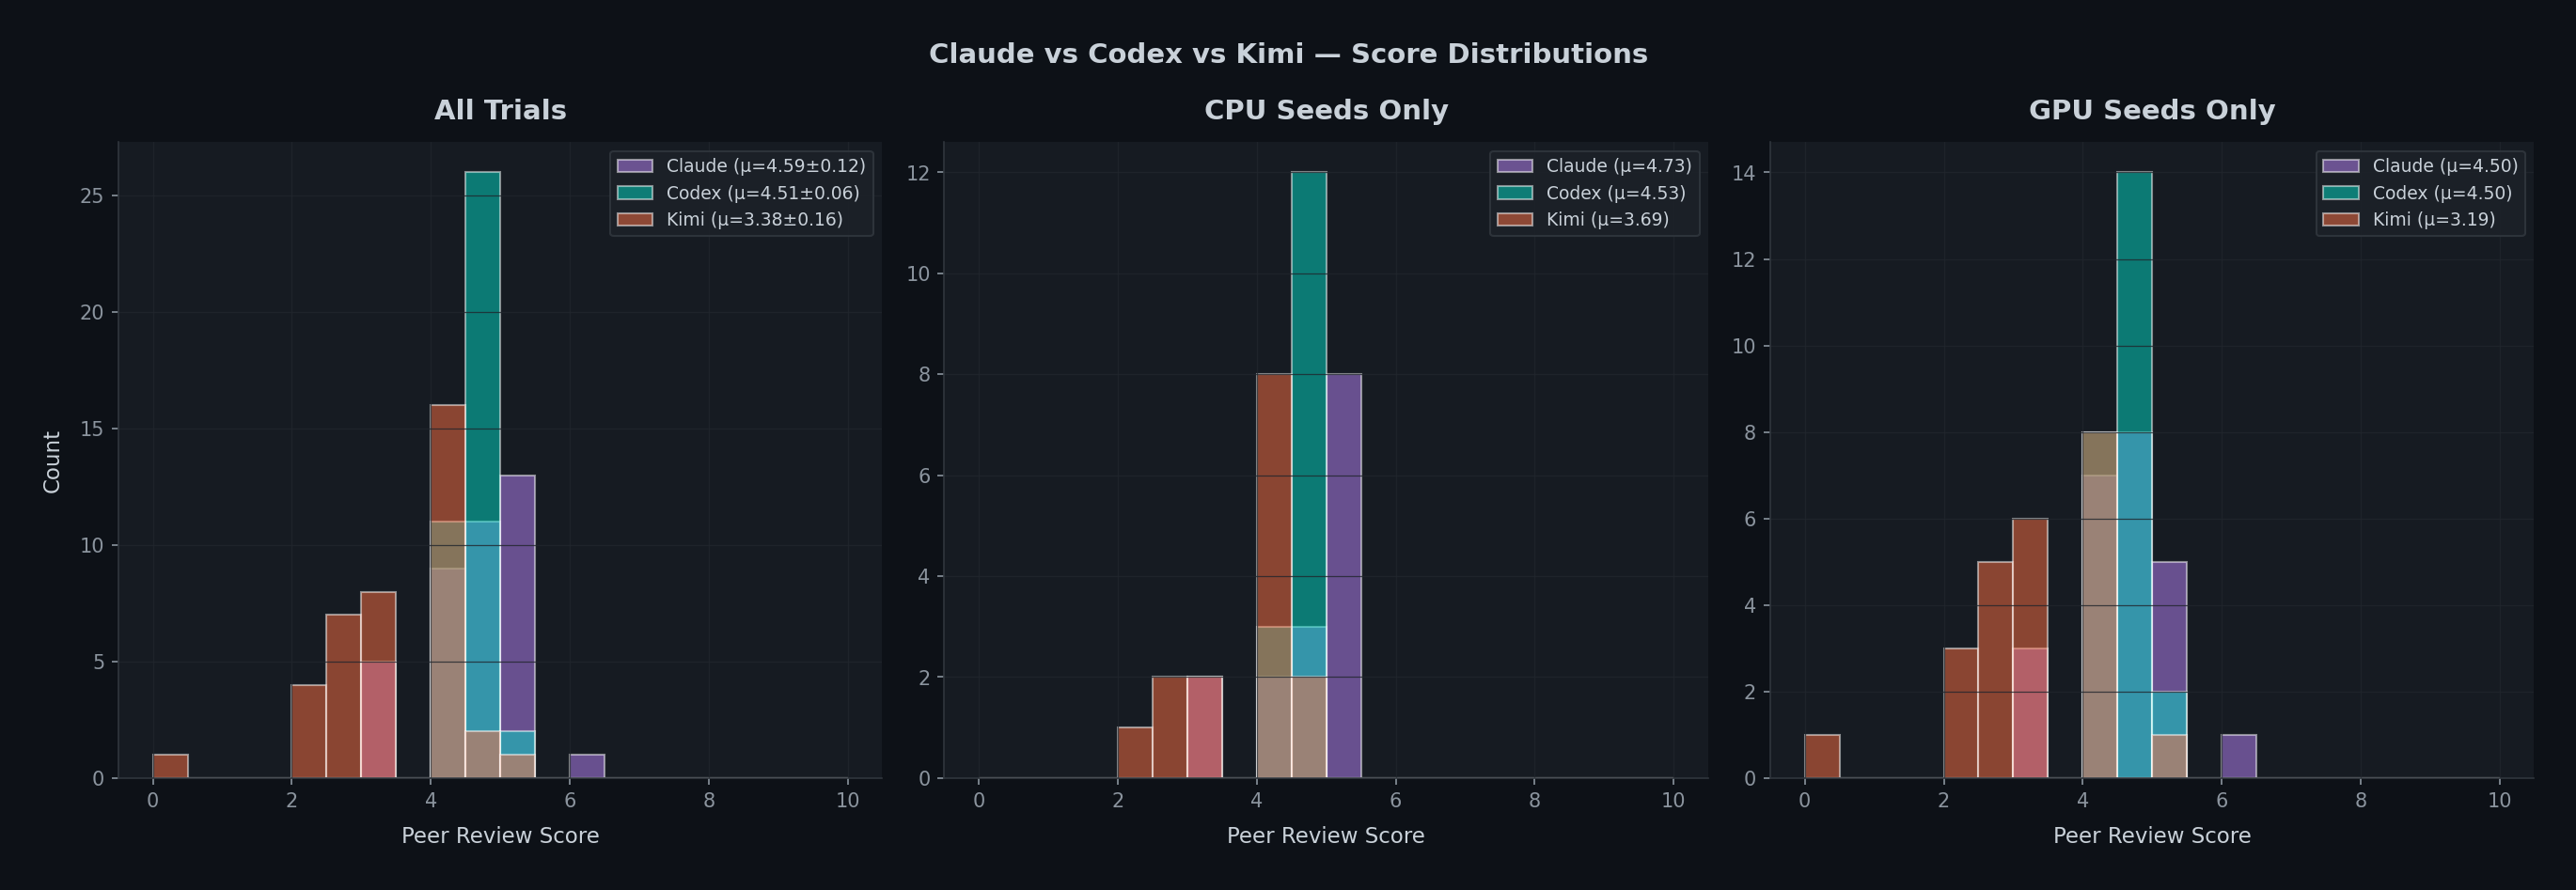
\includegraphics[width=\linewidth]{comparison_3way_score_distributions.png}
\caption{Three-agent score distributions}
\end{subfigure}
\caption{Additional distribution and domain views.}
\end{figure}

\begin{figure}[h]
\centering
\begin{subfigure}{0.48\linewidth}
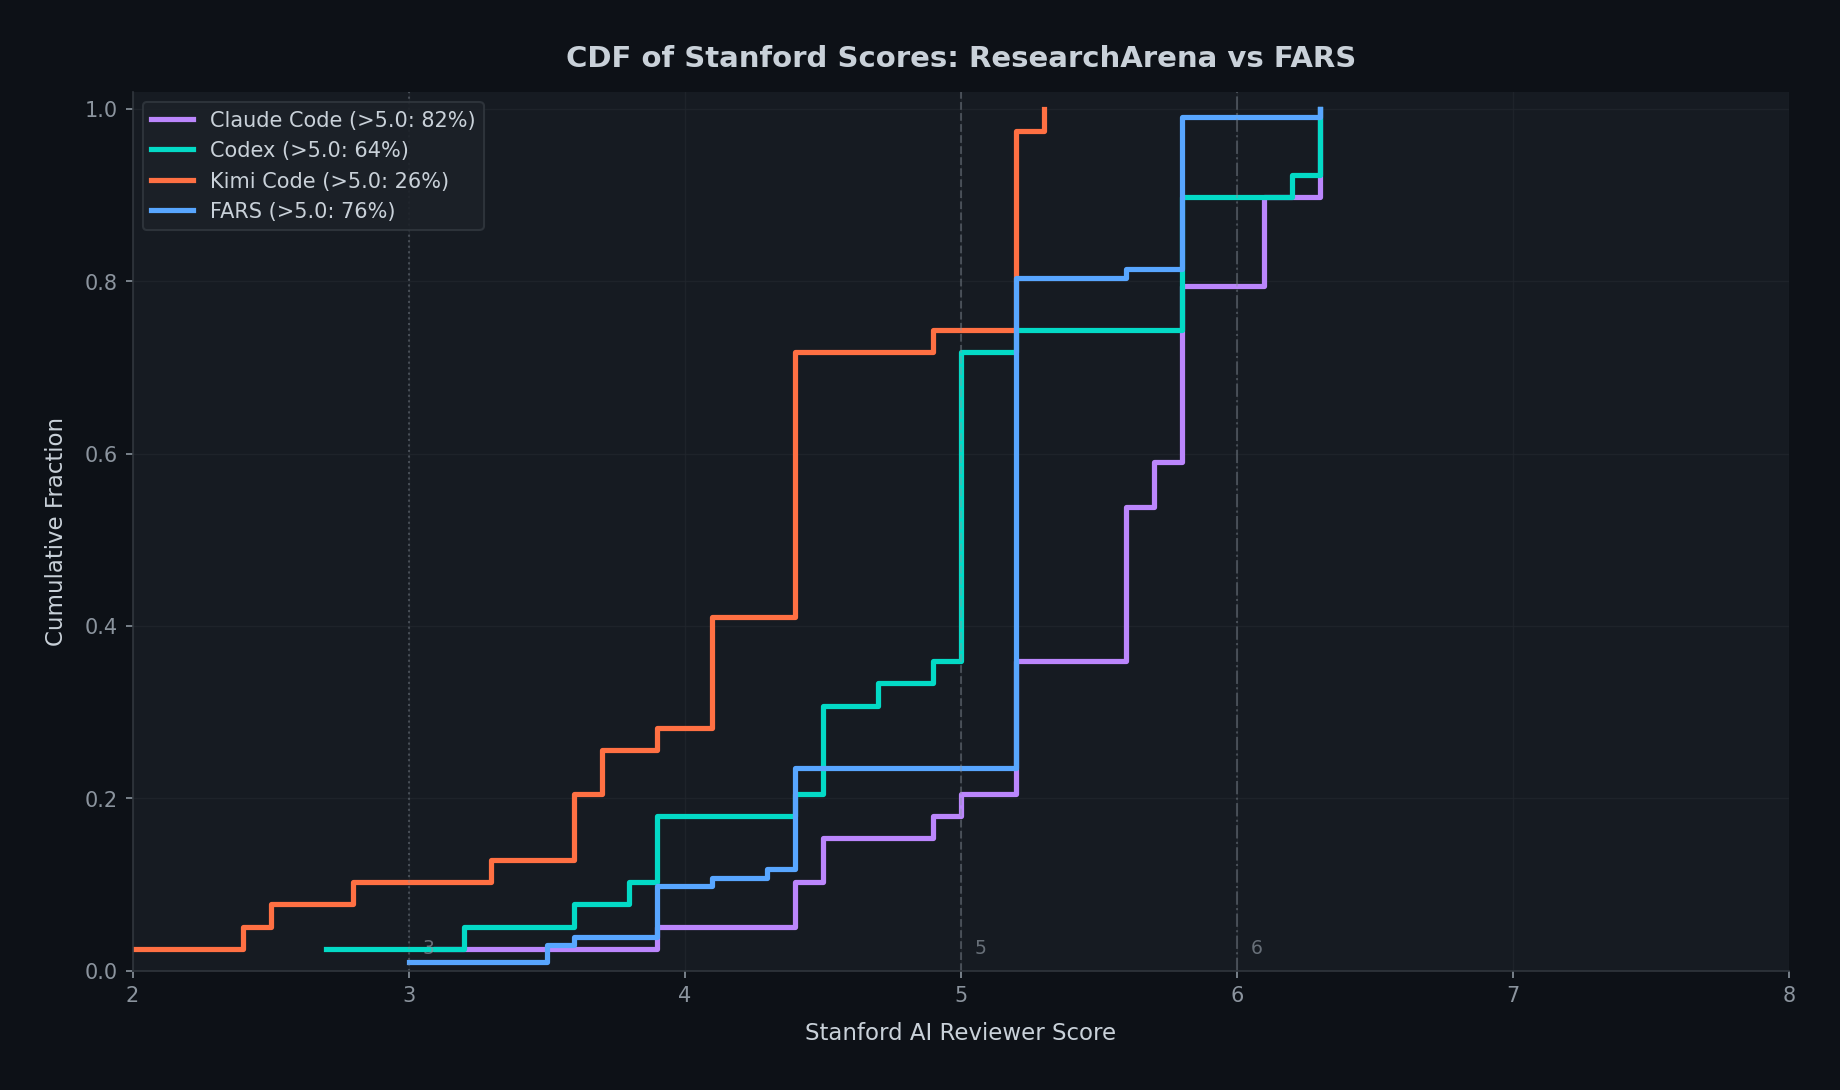
\includegraphics[width=\linewidth]{cdf_comparison.png}
\caption{CDF comparison}
\end{subfigure}
\hfill
\begin{subfigure}{0.48\linewidth}

\includegraphics[width=\linewidth]{violin_vs_fars.png}
\caption{Violin comparison with FARS}
\end{subfigure}
\caption{Secondary \sar\ comparison plots. These are supporting views rather than the central evaluation target.}
\end{figure}

\begin{figure}[h]
\centering
\begin{subfigure}{0.48\linewidth}
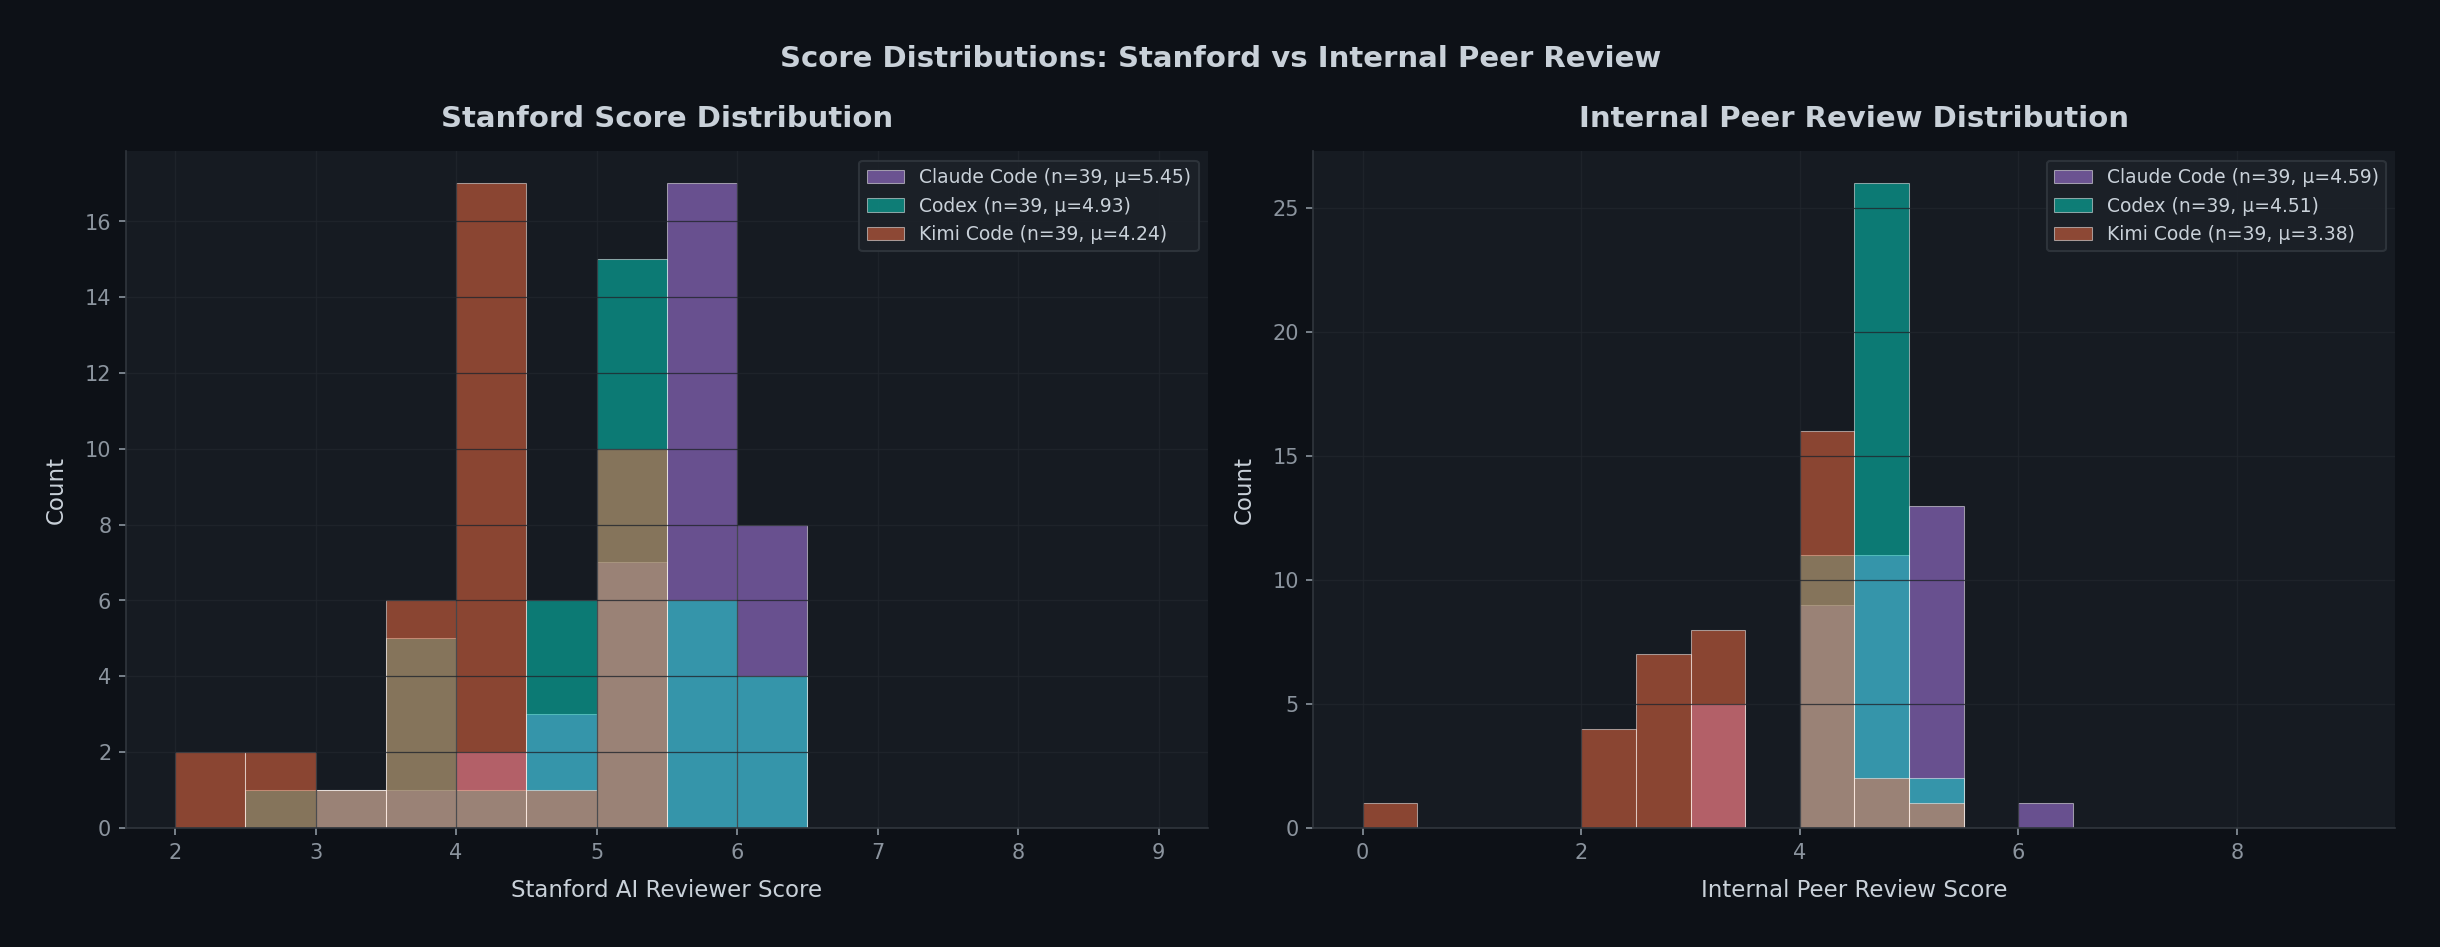
\includegraphics[width=\linewidth]{score_distributions.png}
\caption{Aggregate score distributions}
\end{subfigure}
\hfill
\begin{subfigure}{0.48\linewidth}

\includegraphics[width=\linewidth]{weakness_themes.png}
\caption{Weakness themes}
\end{subfigure}
\caption{Aggregate score and weakness-theme plots.}
\end{figure}

\subsection{Agent-Specific Score, Domain, and Failure Plots}

\begin{figure}[h]
\centering
\begin{subfigure}{0.32\linewidth}
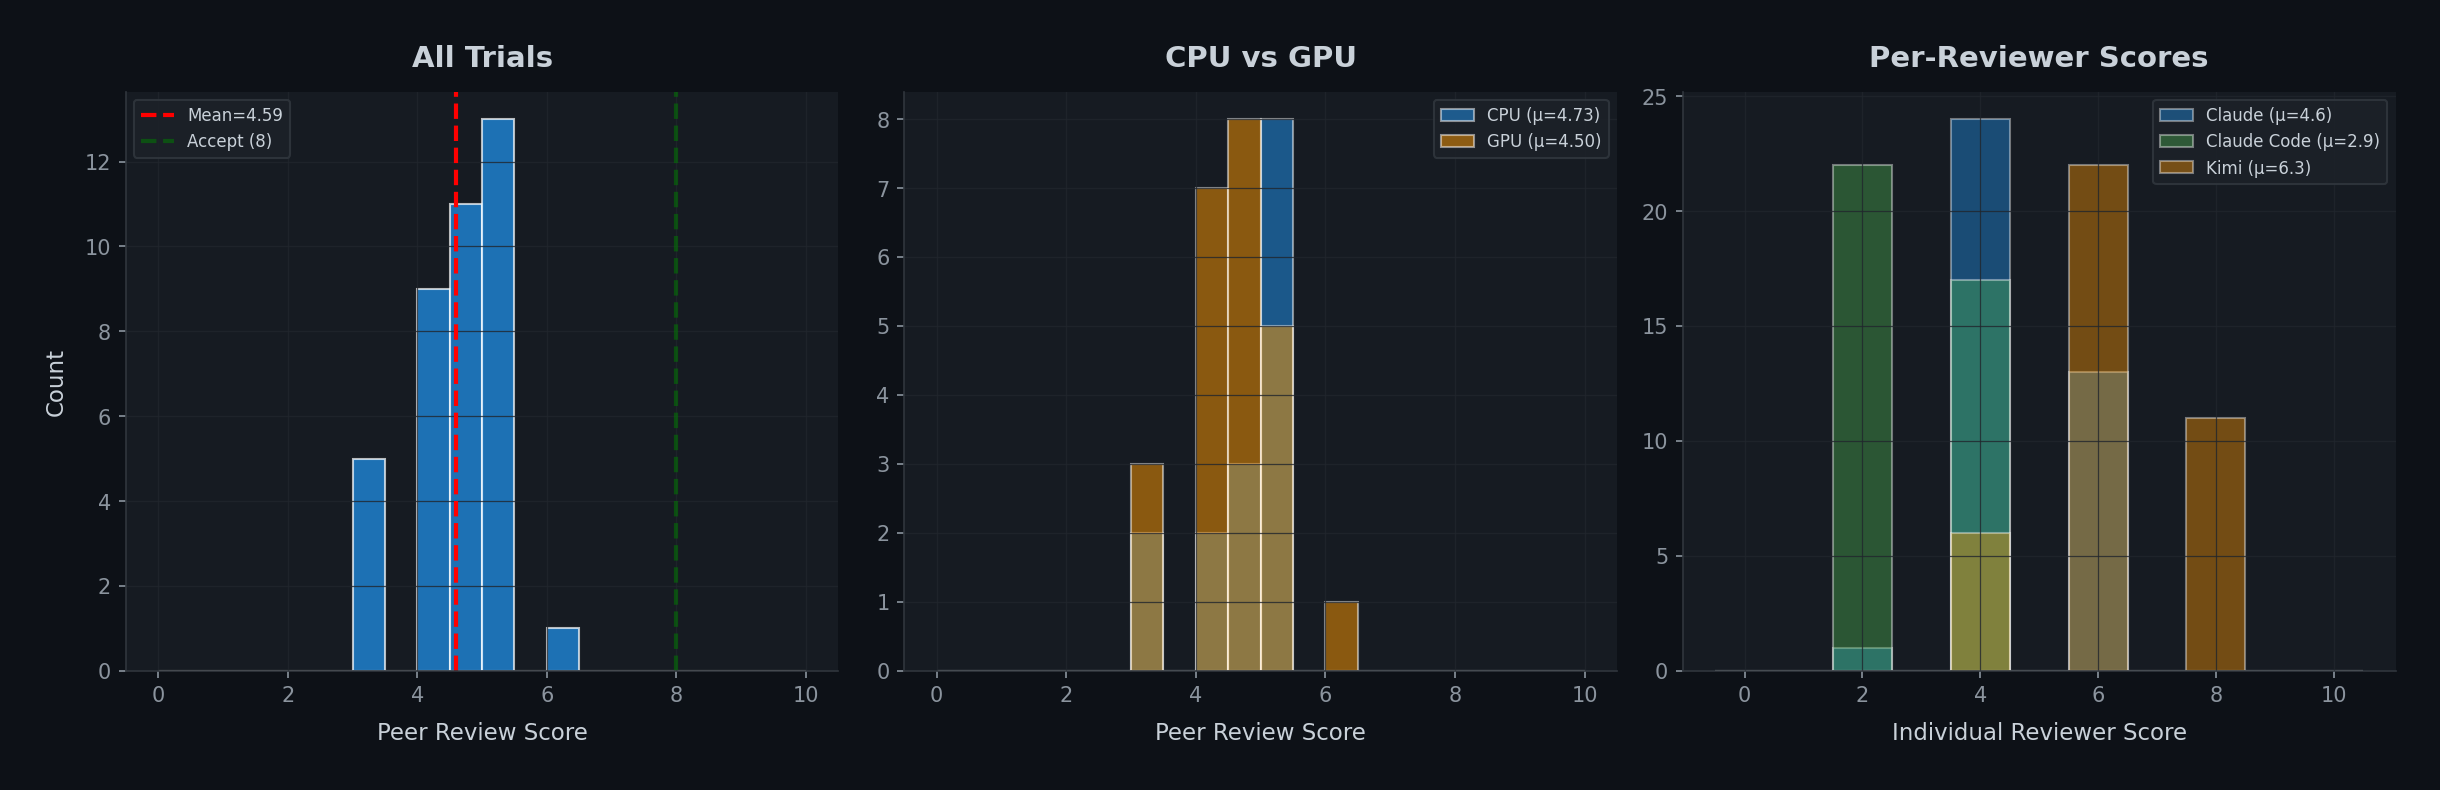
\includegraphics[width=\linewidth]{claude_score_distributions.png}
\caption{Claude}
\end{subfigure}
\begin{subfigure}{0.32\linewidth}
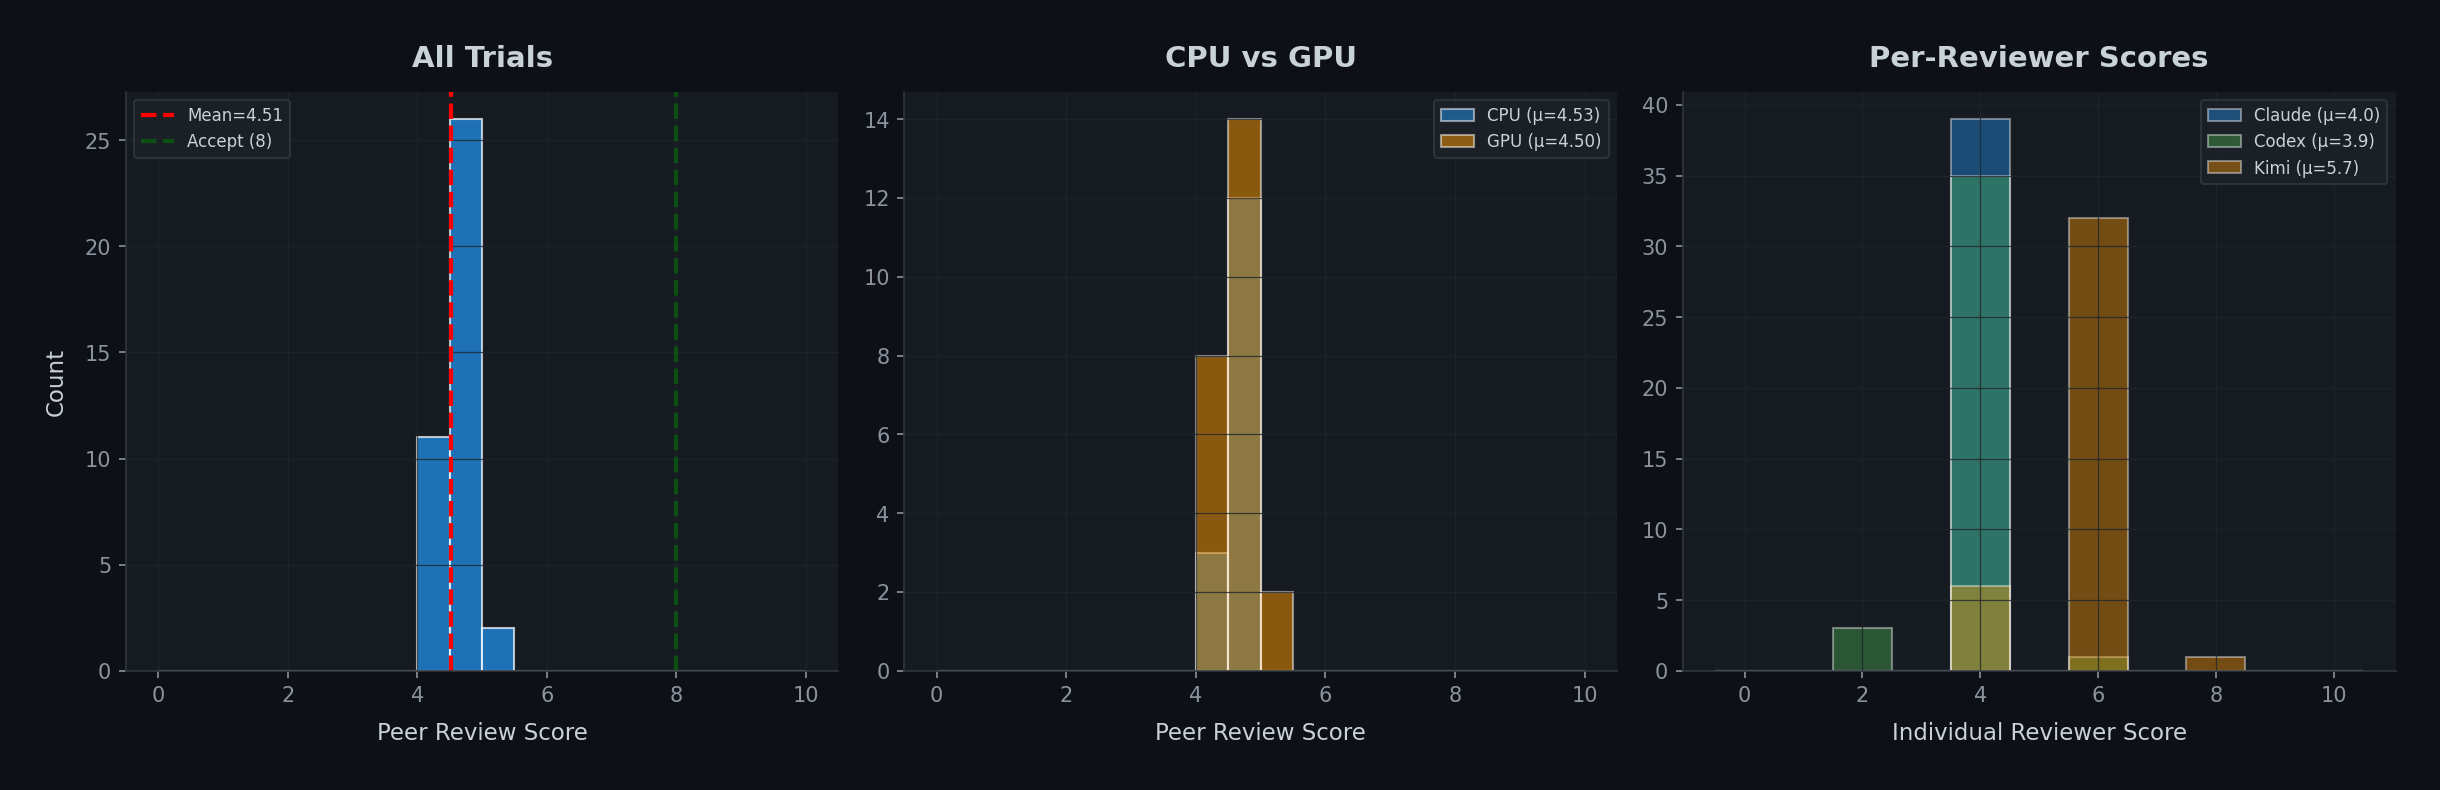
\includegraphics[width=\linewidth]{codex_score_distributions.png}
\caption{Codex}
\end{subfigure}
\begin{subfigure}{0.32\linewidth}
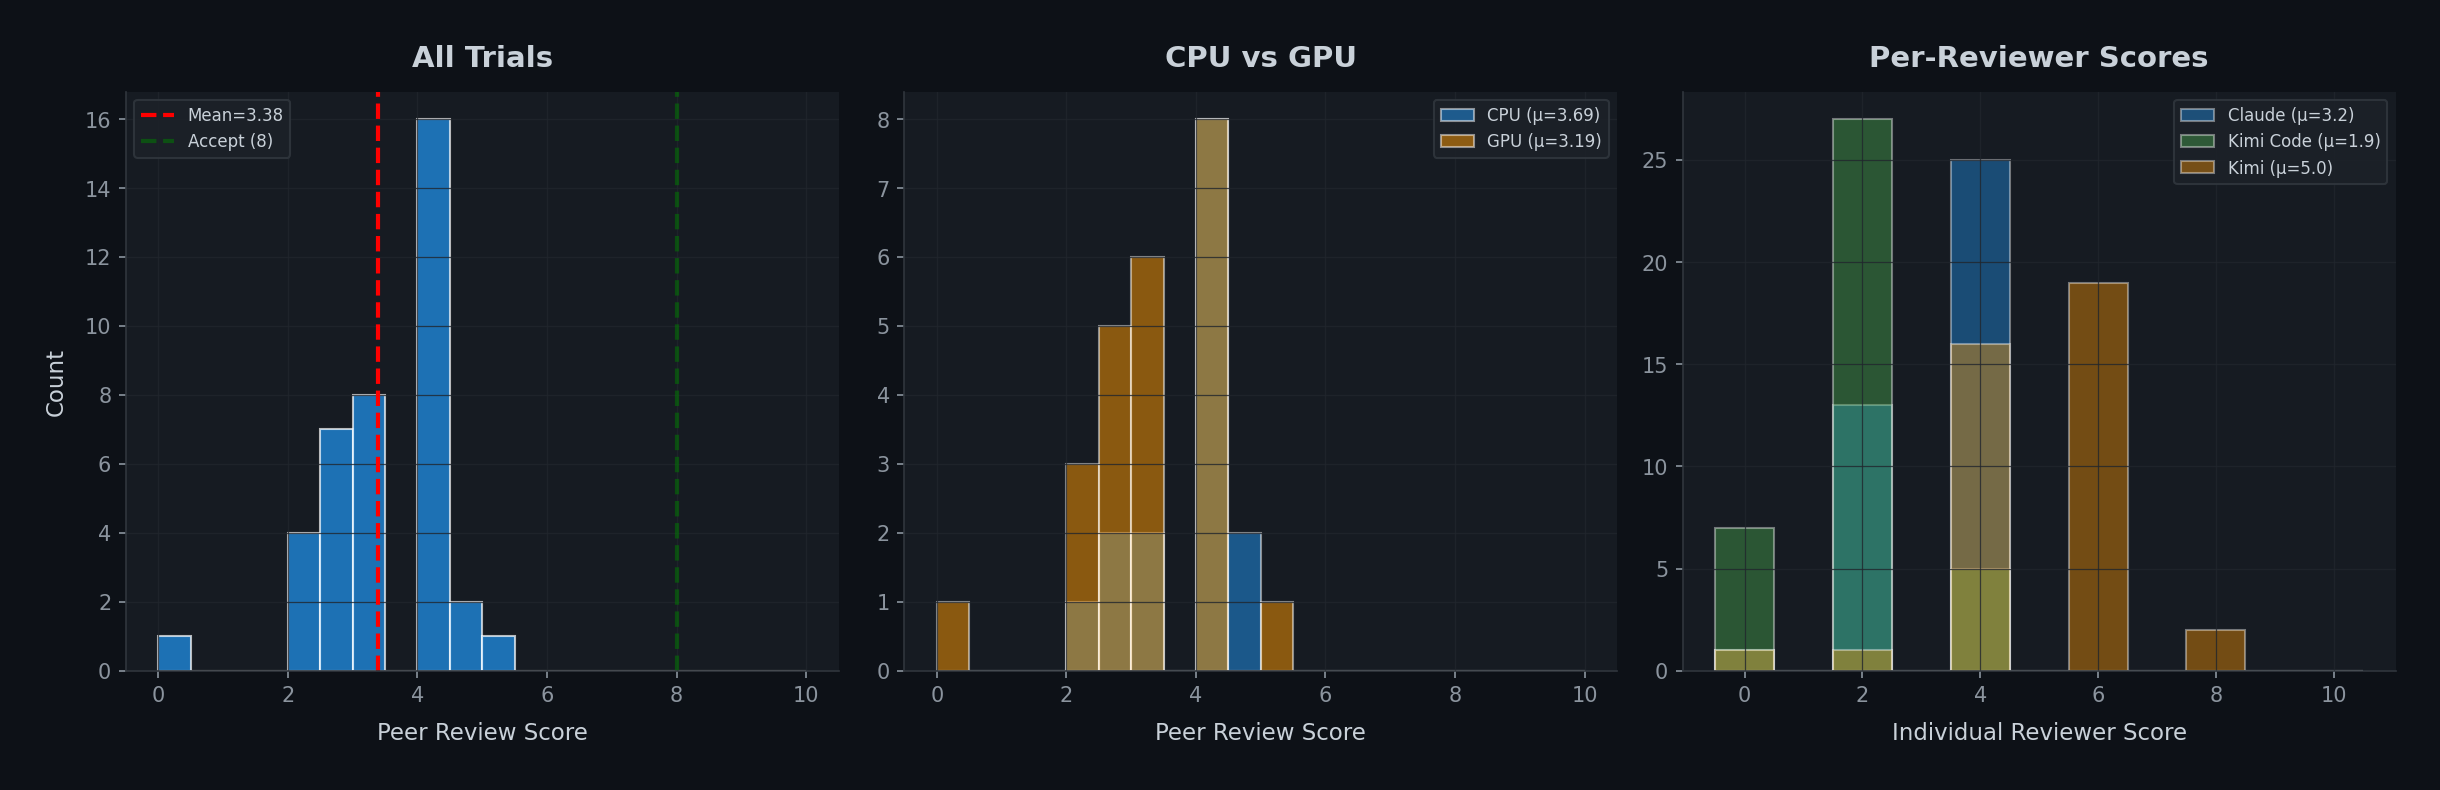
\includegraphics[width=\linewidth]{kimi_score_distributions.png}
\caption{Kimi}
\end{subfigure}
\caption{Agent-specific score distributions.}
\end{figure}

\begin{figure}[h]
\centering
\begin{subfigure}{0.32\linewidth}
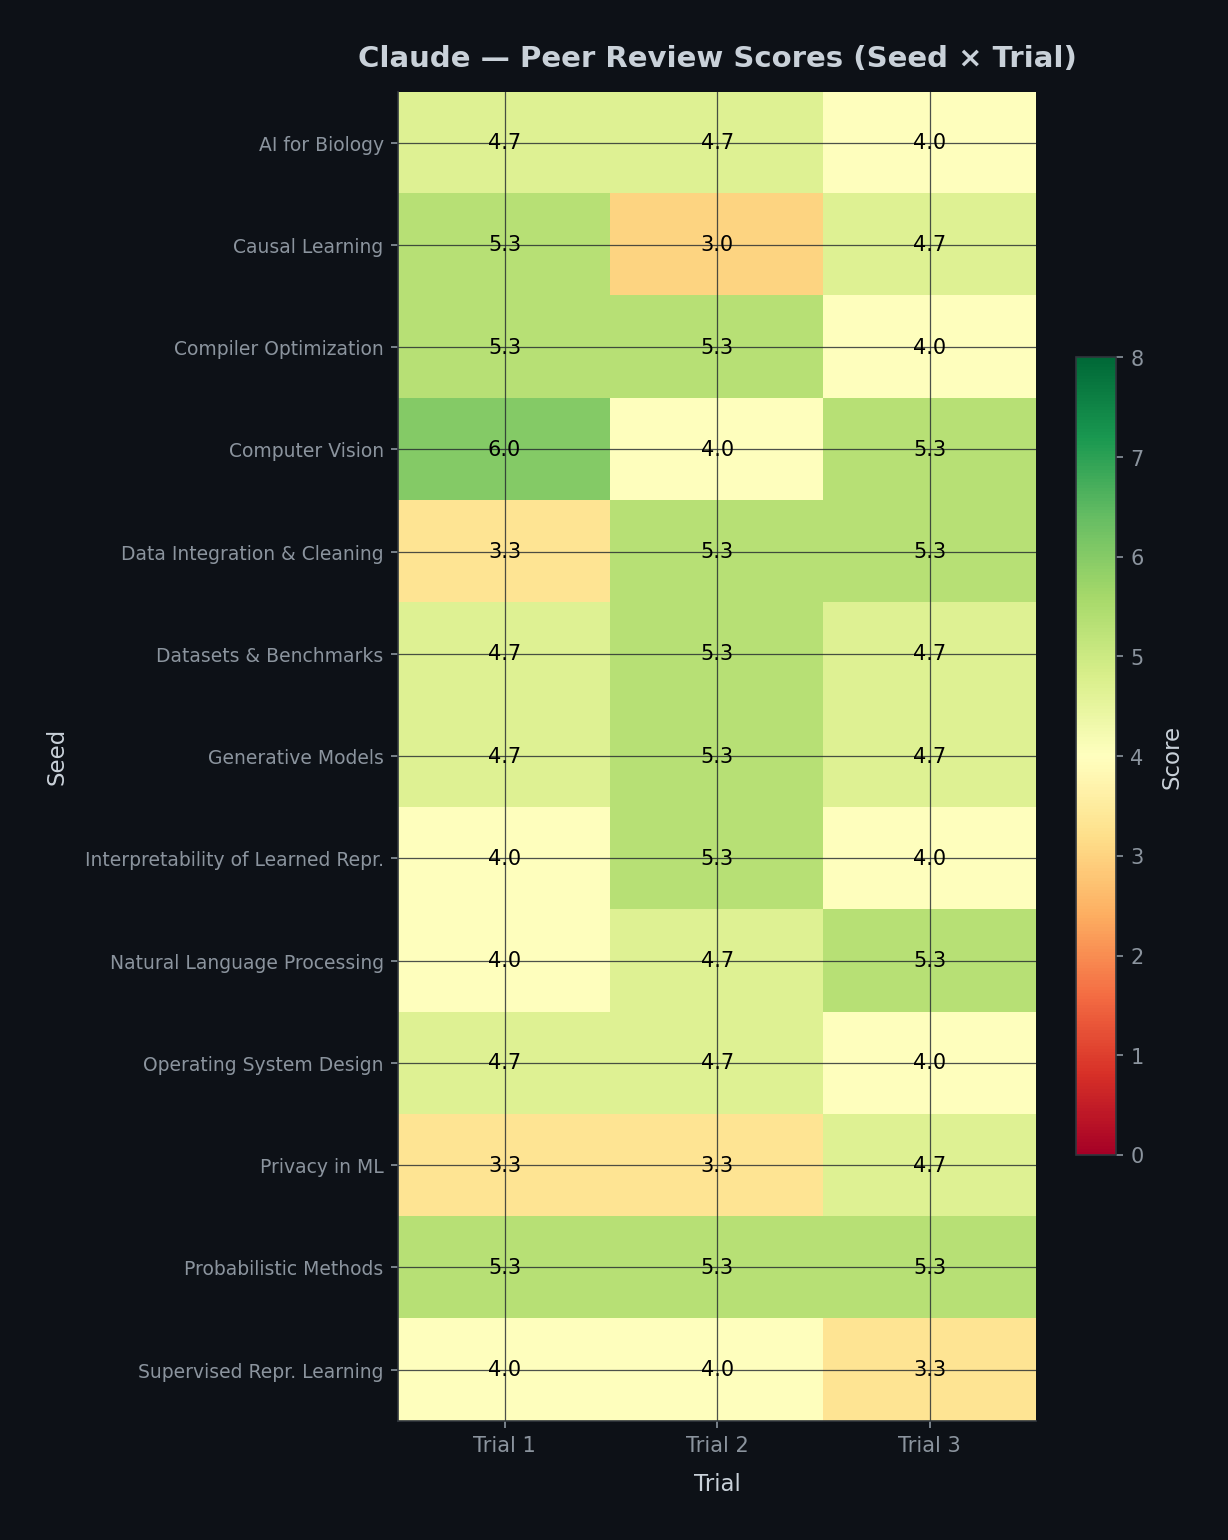
\includegraphics[width=\linewidth]{claude_score_heatmap.png}
\caption{Claude}
\end{subfigure}
\begin{subfigure}{0.32\linewidth}
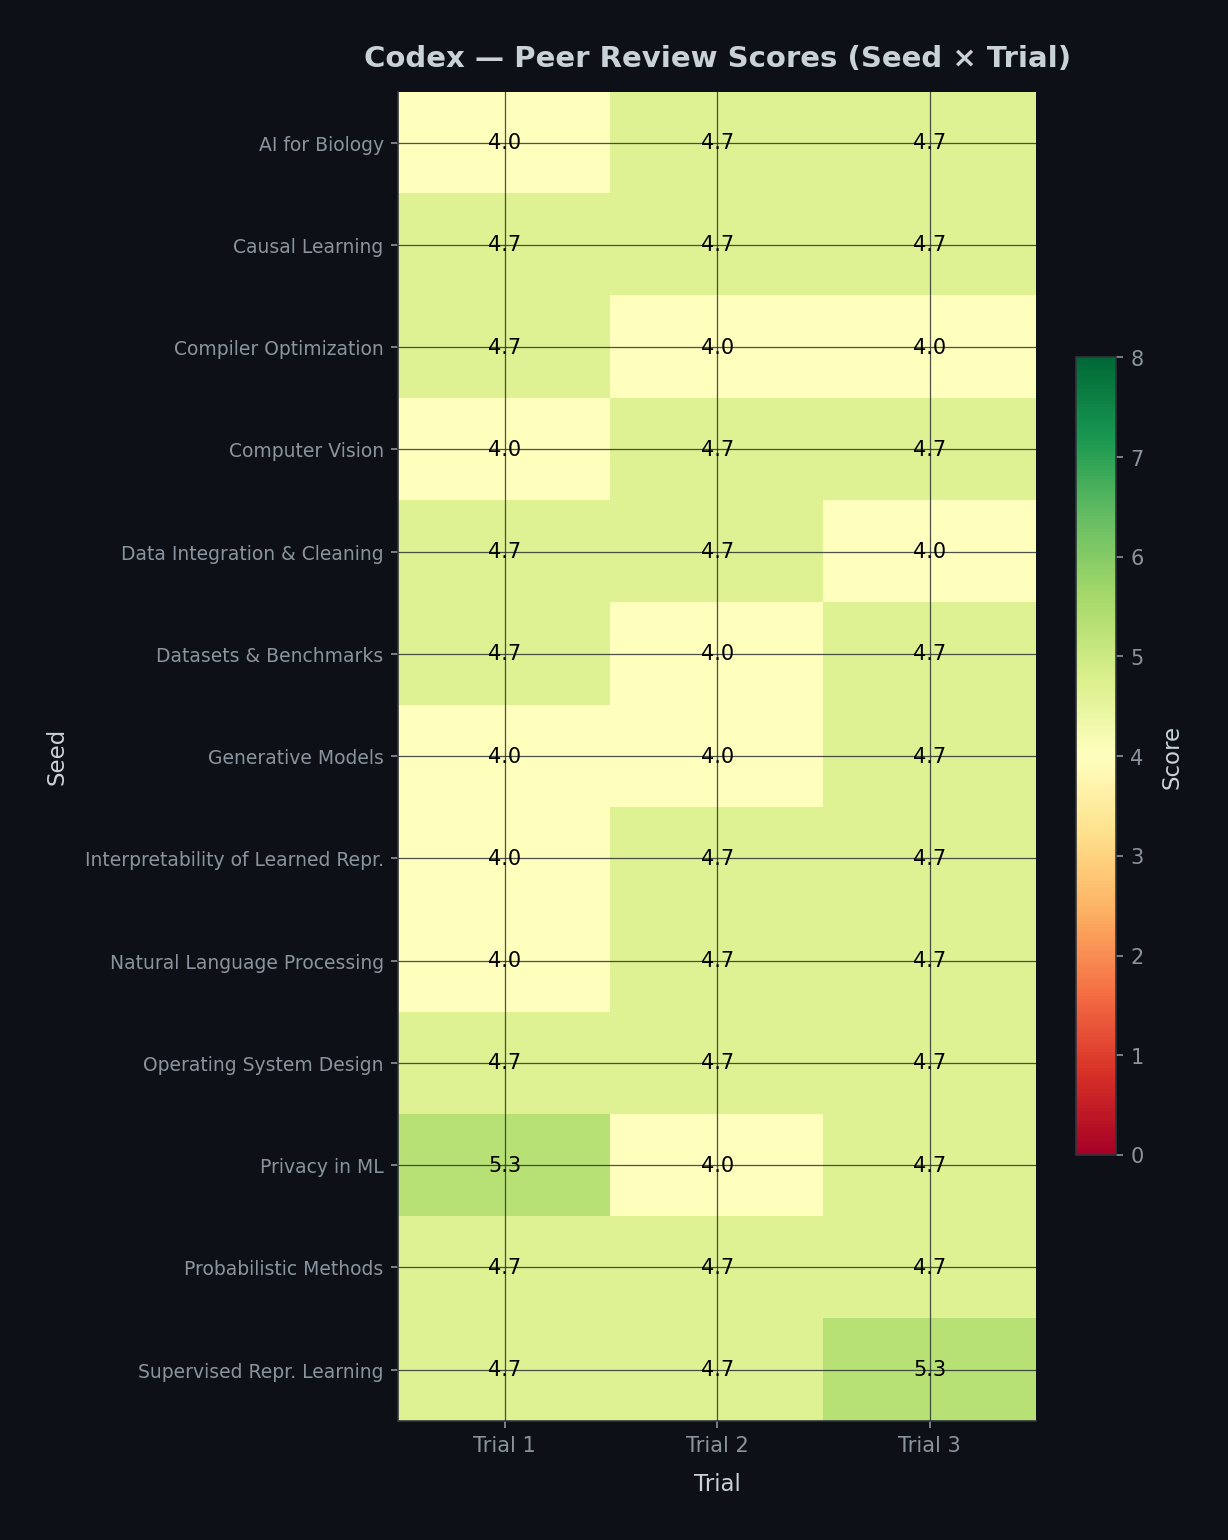
\includegraphics[width=\linewidth]{codex_score_heatmap.png}
\caption{Codex}
\end{subfigure}
\begin{subfigure}{0.32\linewidth}
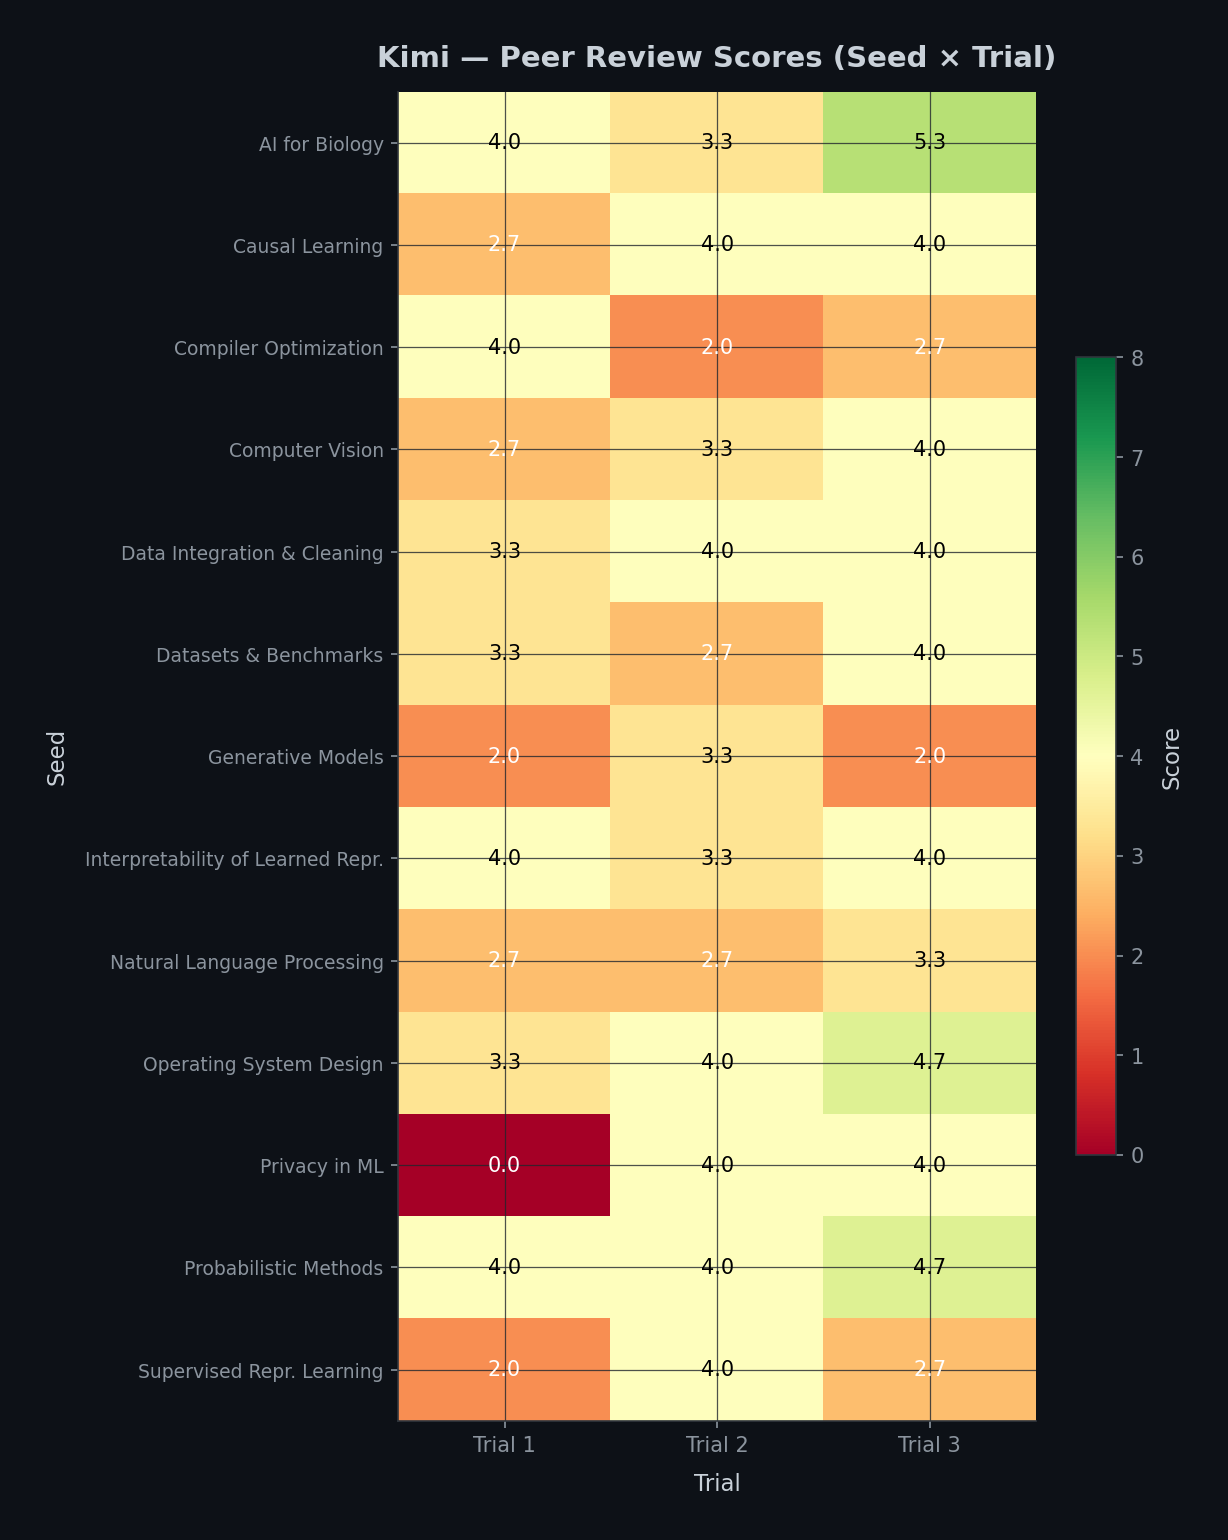
\includegraphics[width=\linewidth]{kimi_score_heatmap.png}
\caption{Kimi}
\end{subfigure}
\caption{Agent-specific heatmaps.}
\end{figure}

\begin{figure}[h]
\centering
\begin{subfigure}{0.32\linewidth}
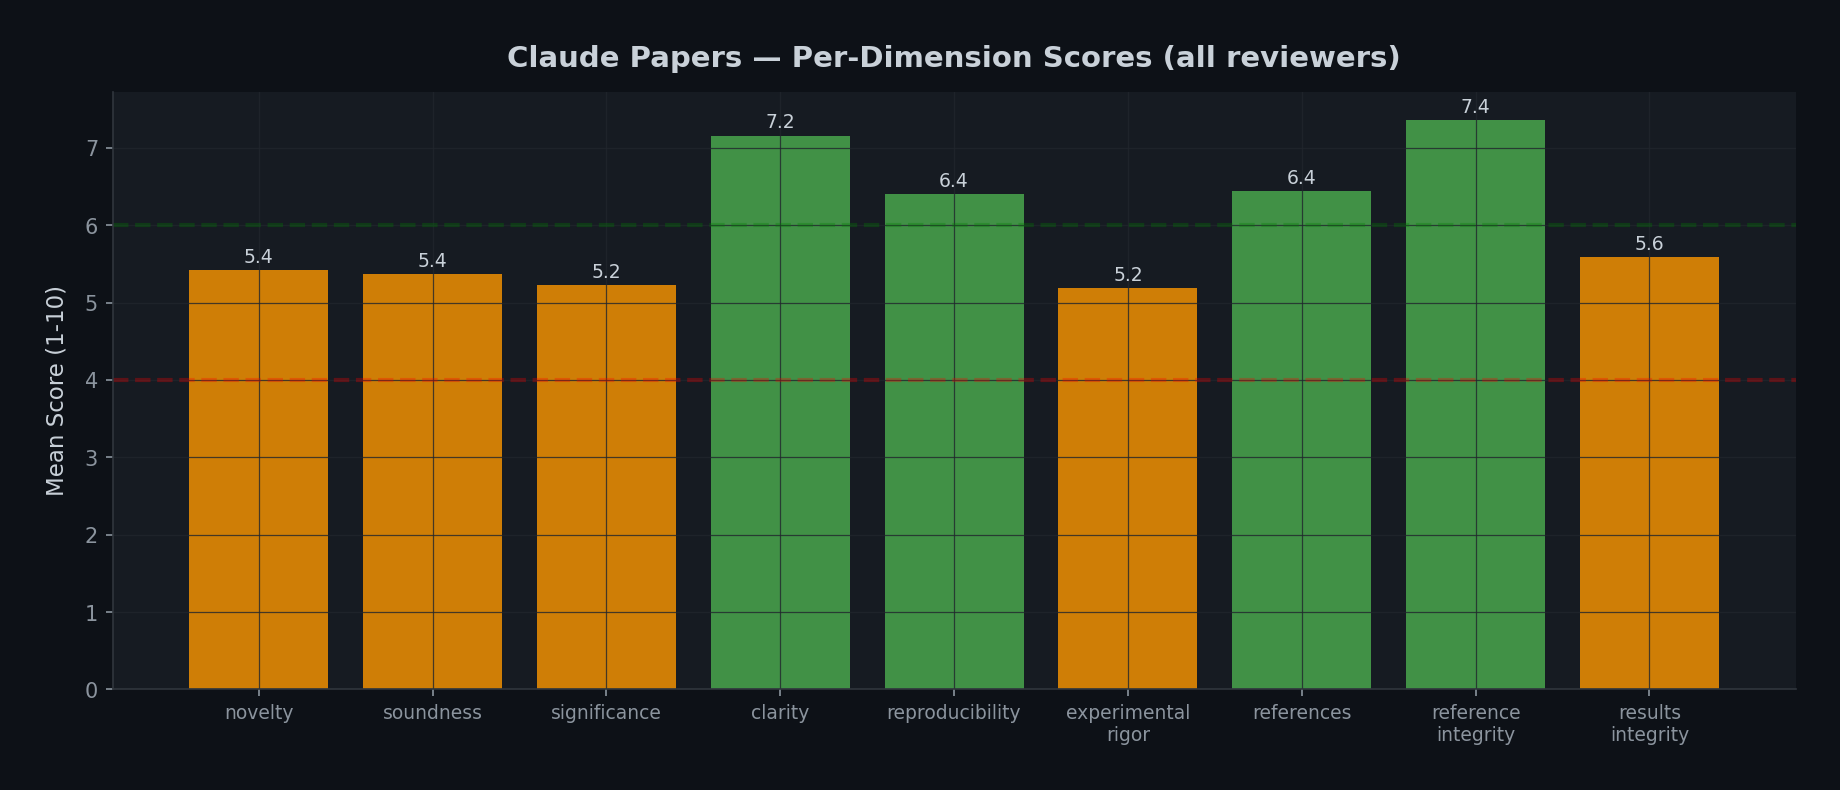
\includegraphics[width=\linewidth]{claude_dimension_scores.png}
\caption{Claude}
\end{subfigure}
\begin{subfigure}{0.32\linewidth}
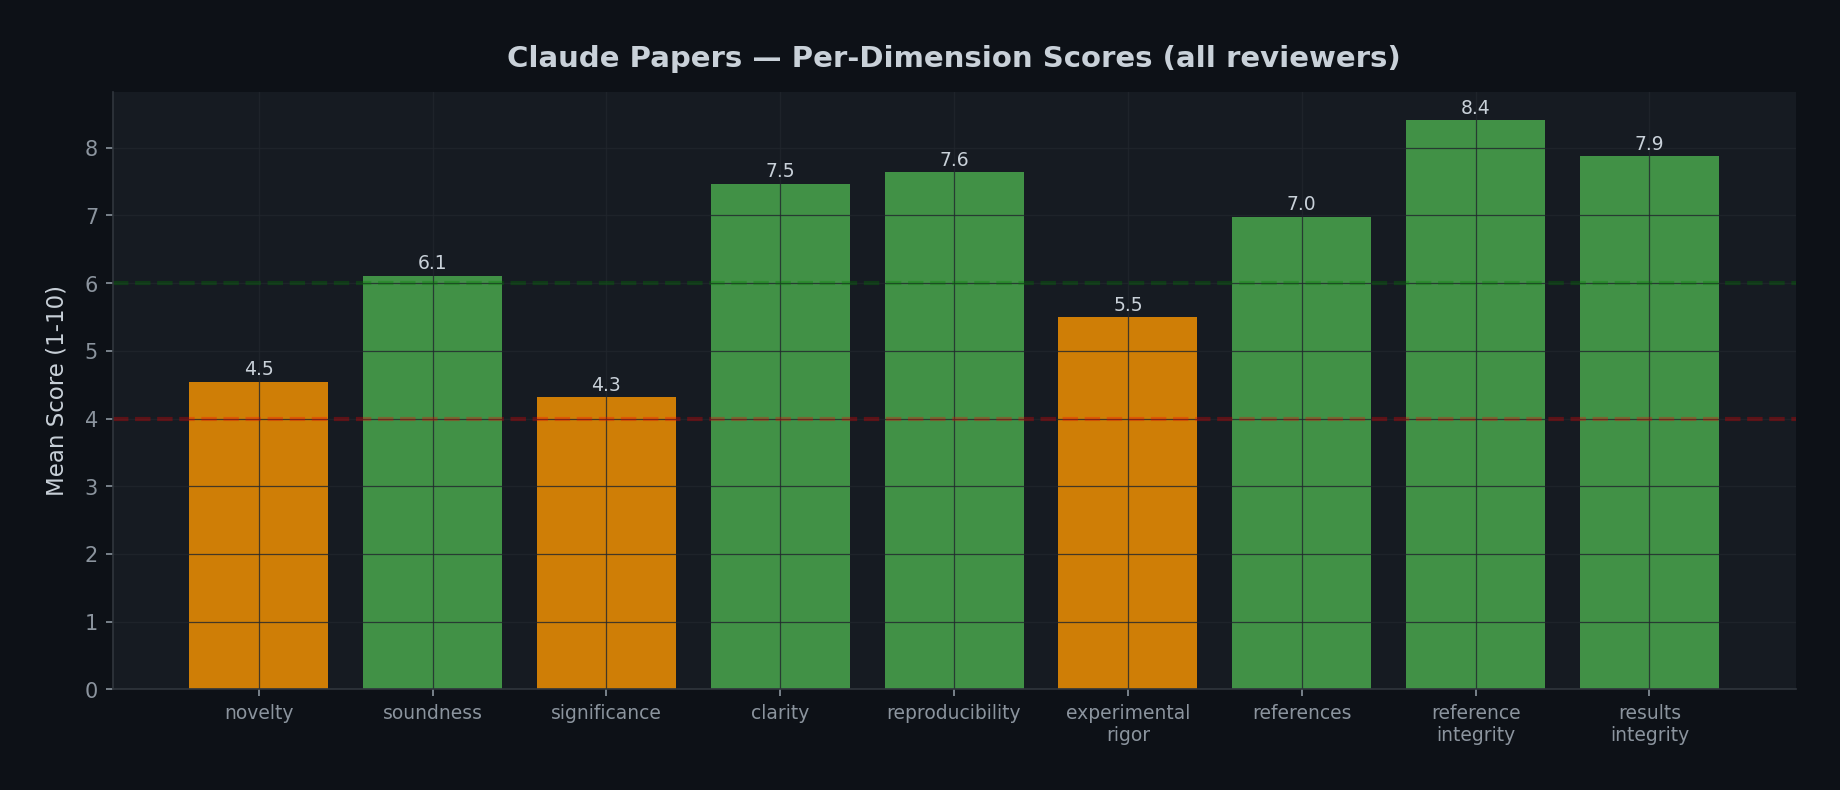
\includegraphics[width=\linewidth]{codex_dimension_scores.png}
\caption{Codex}
\end{subfigure}
\begin{subfigure}{0.32\linewidth}
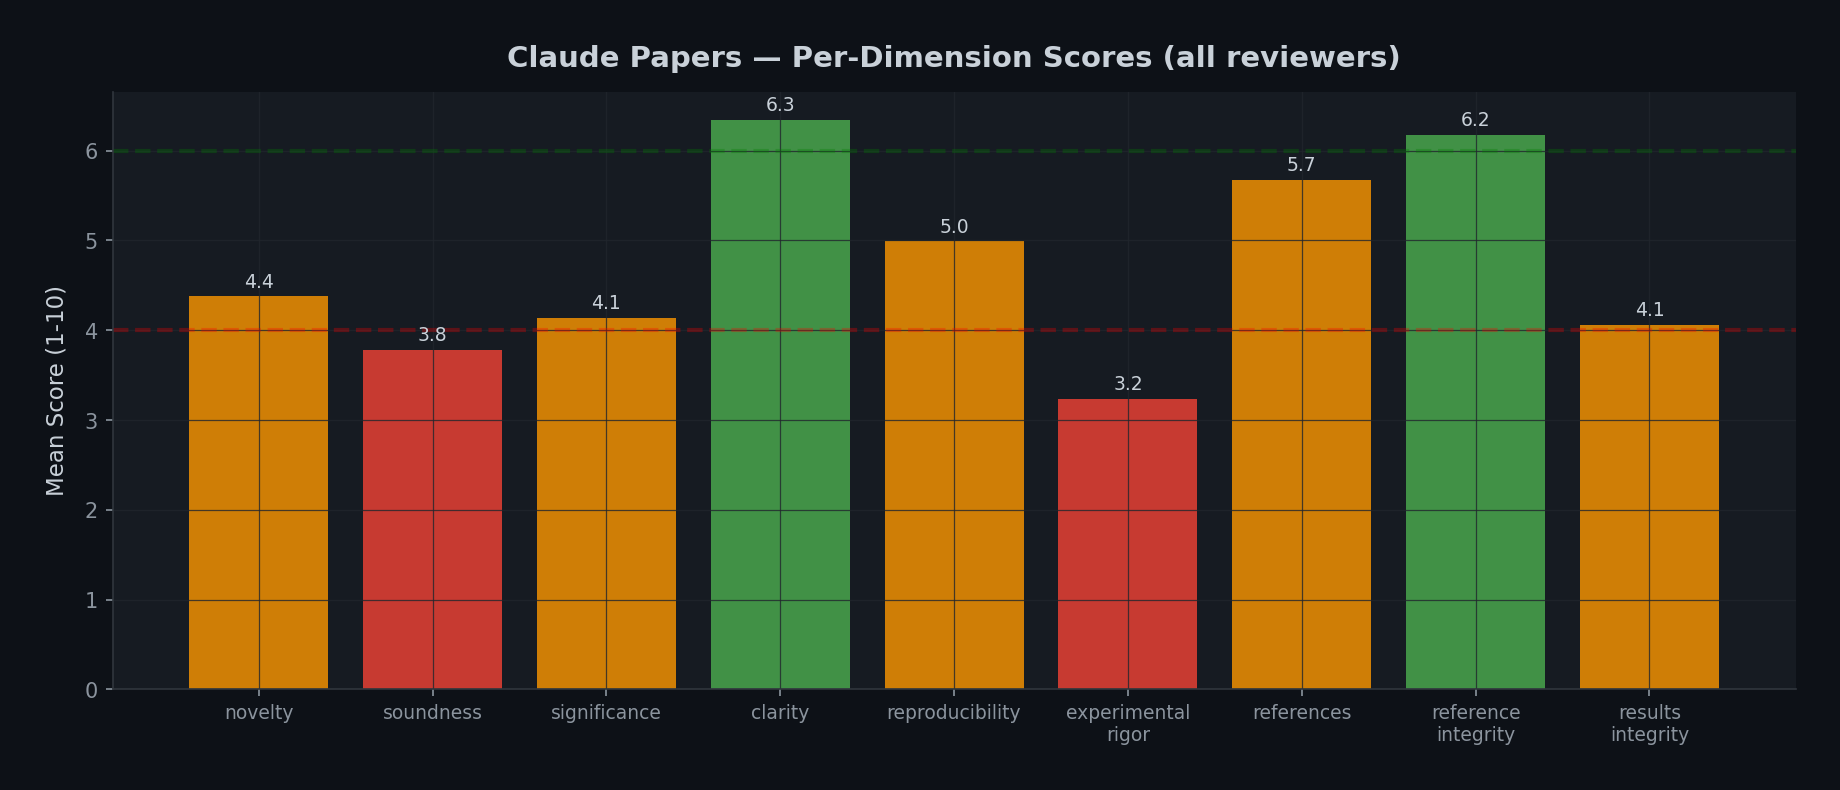
\includegraphics[width=\linewidth]{kimi_dimension_scores.png}
\caption{Kimi}
\end{subfigure}
\caption{Agent-specific dimension scores.}
\end{figure}

\begin{figure}[h]
\centering
\begin{subfigure}{0.32\linewidth}
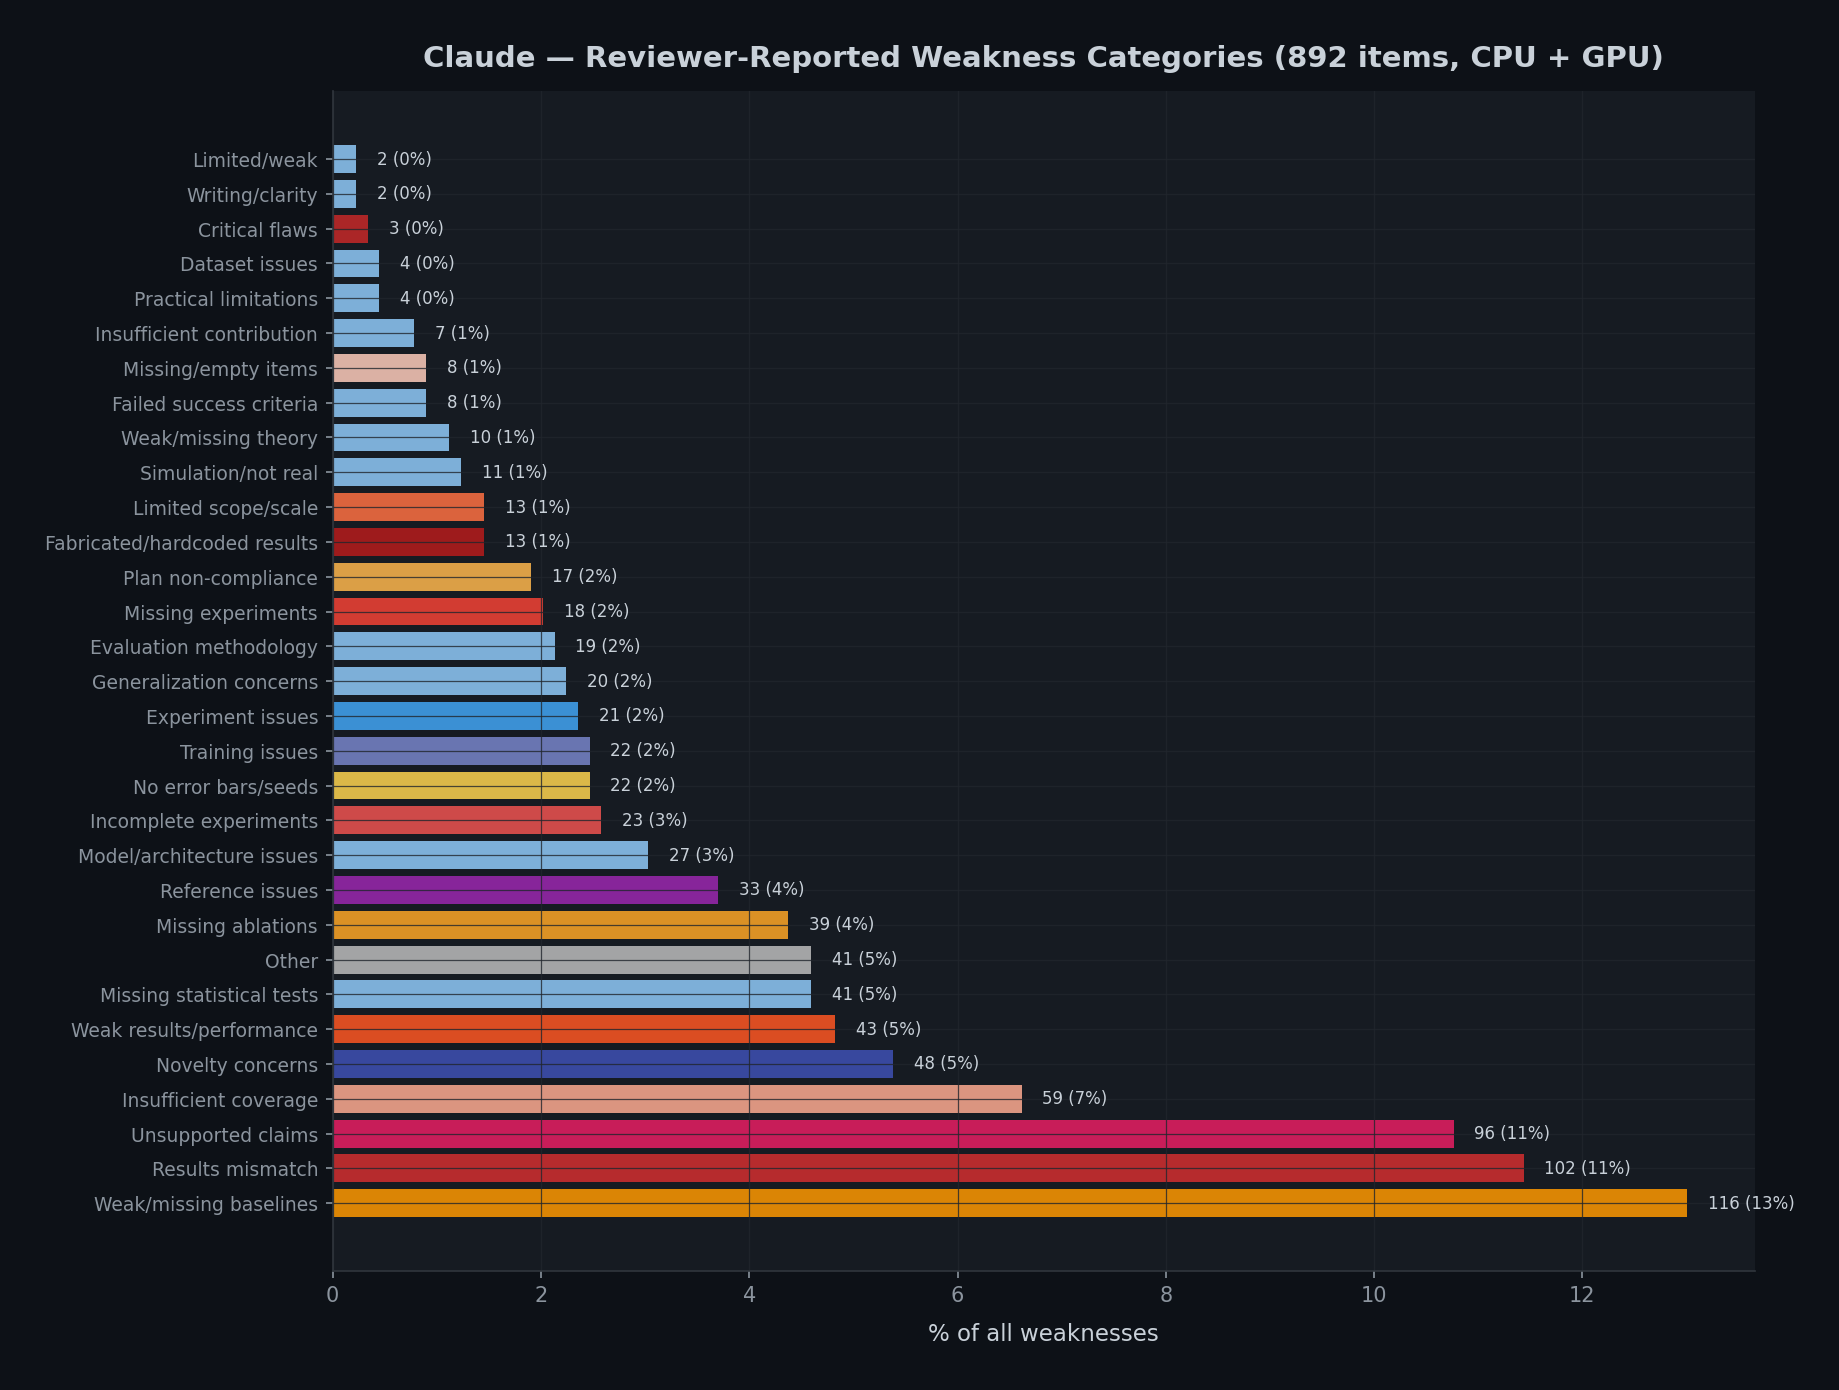
\includegraphics[width=\linewidth]{claude_failure_categories.png}
\caption{Claude}
\end{subfigure}
\begin{subfigure}{0.32\linewidth}
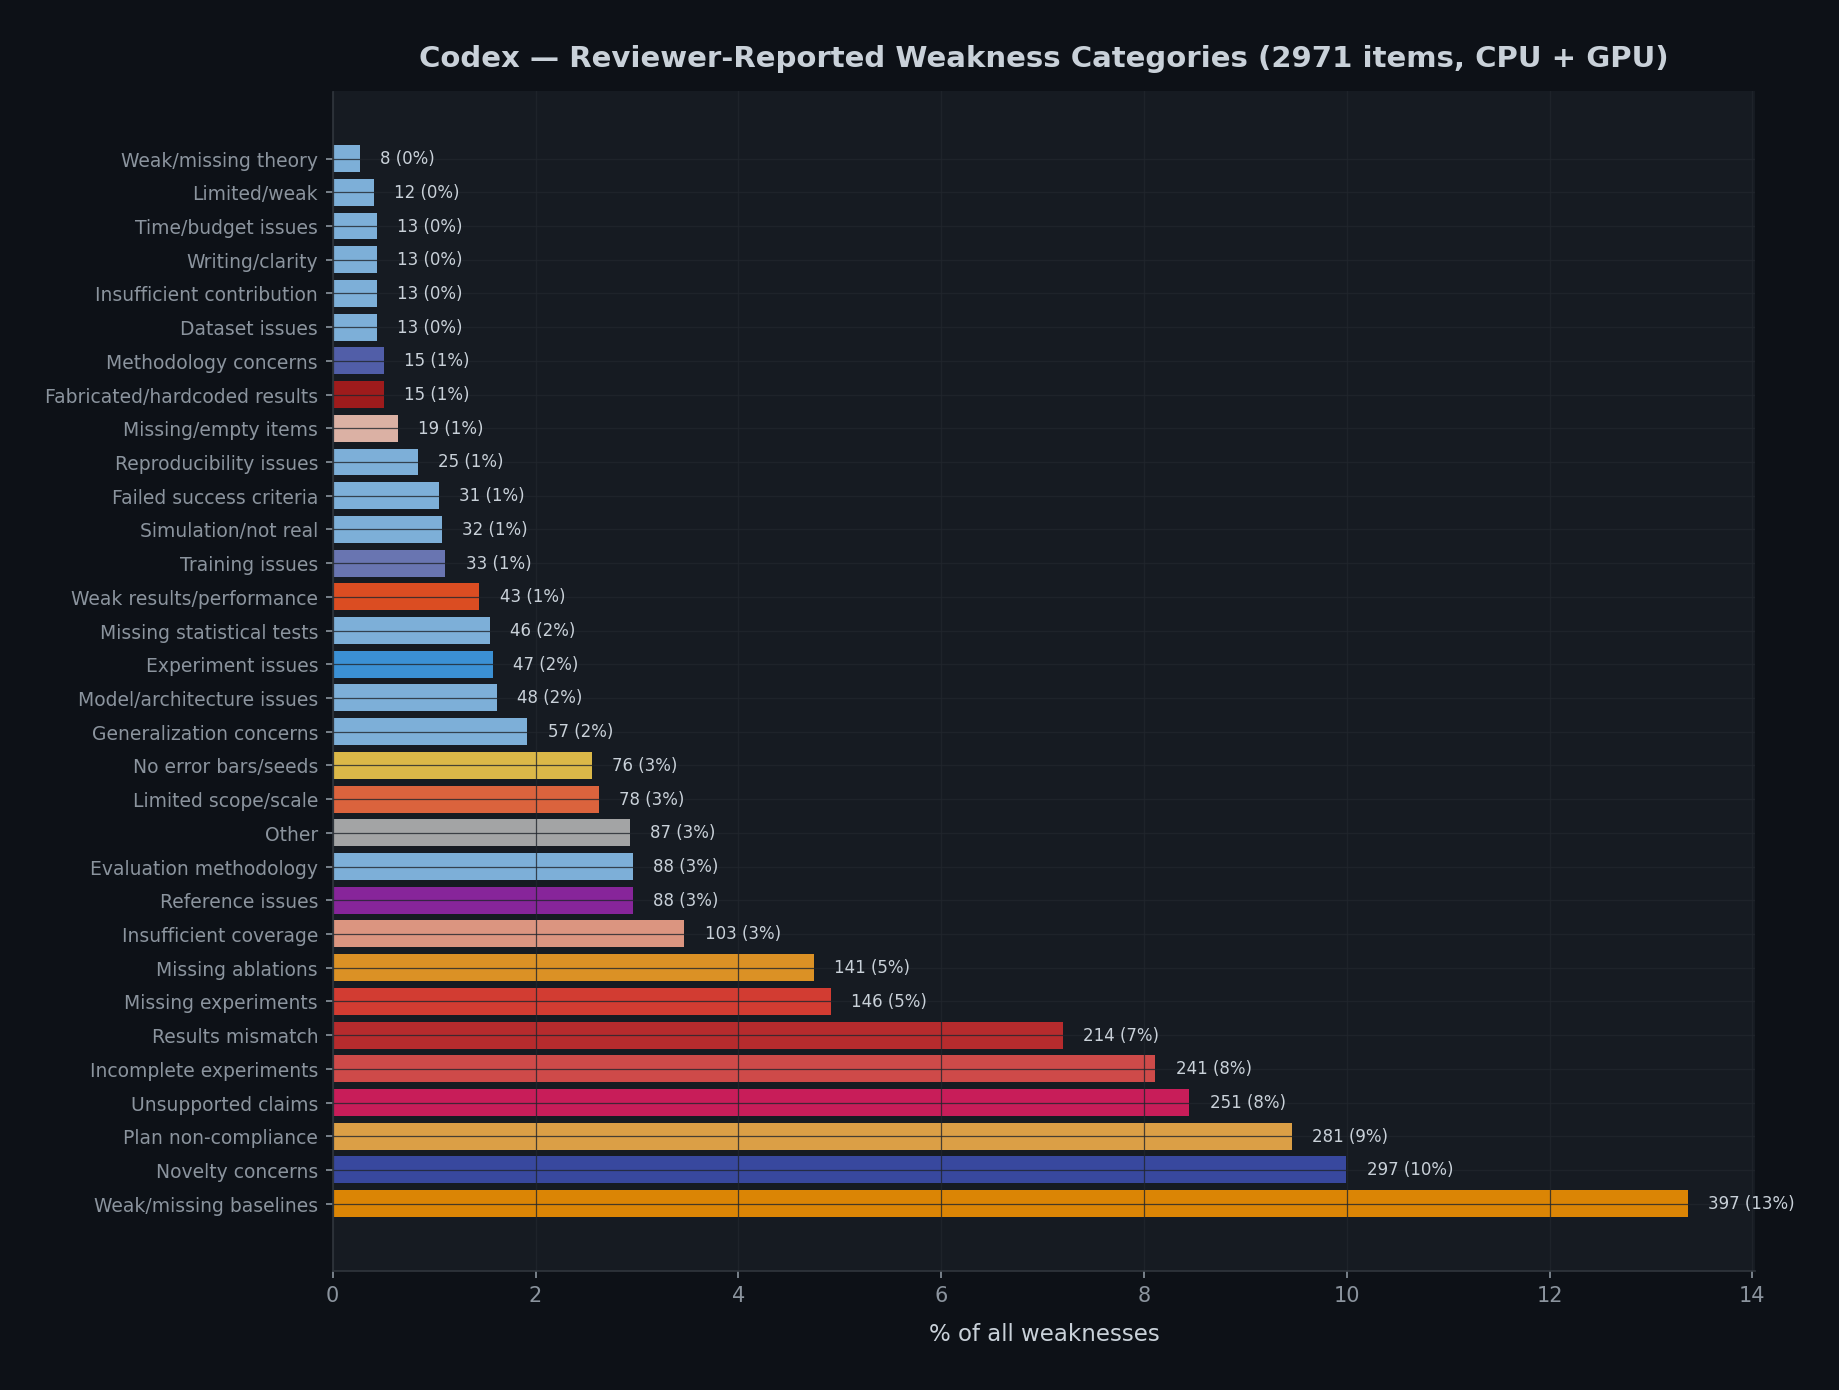
\includegraphics[width=\linewidth]{codex_failure_categories.png}
\caption{Codex}
\end{subfigure}
\begin{subfigure}{0.32\linewidth}
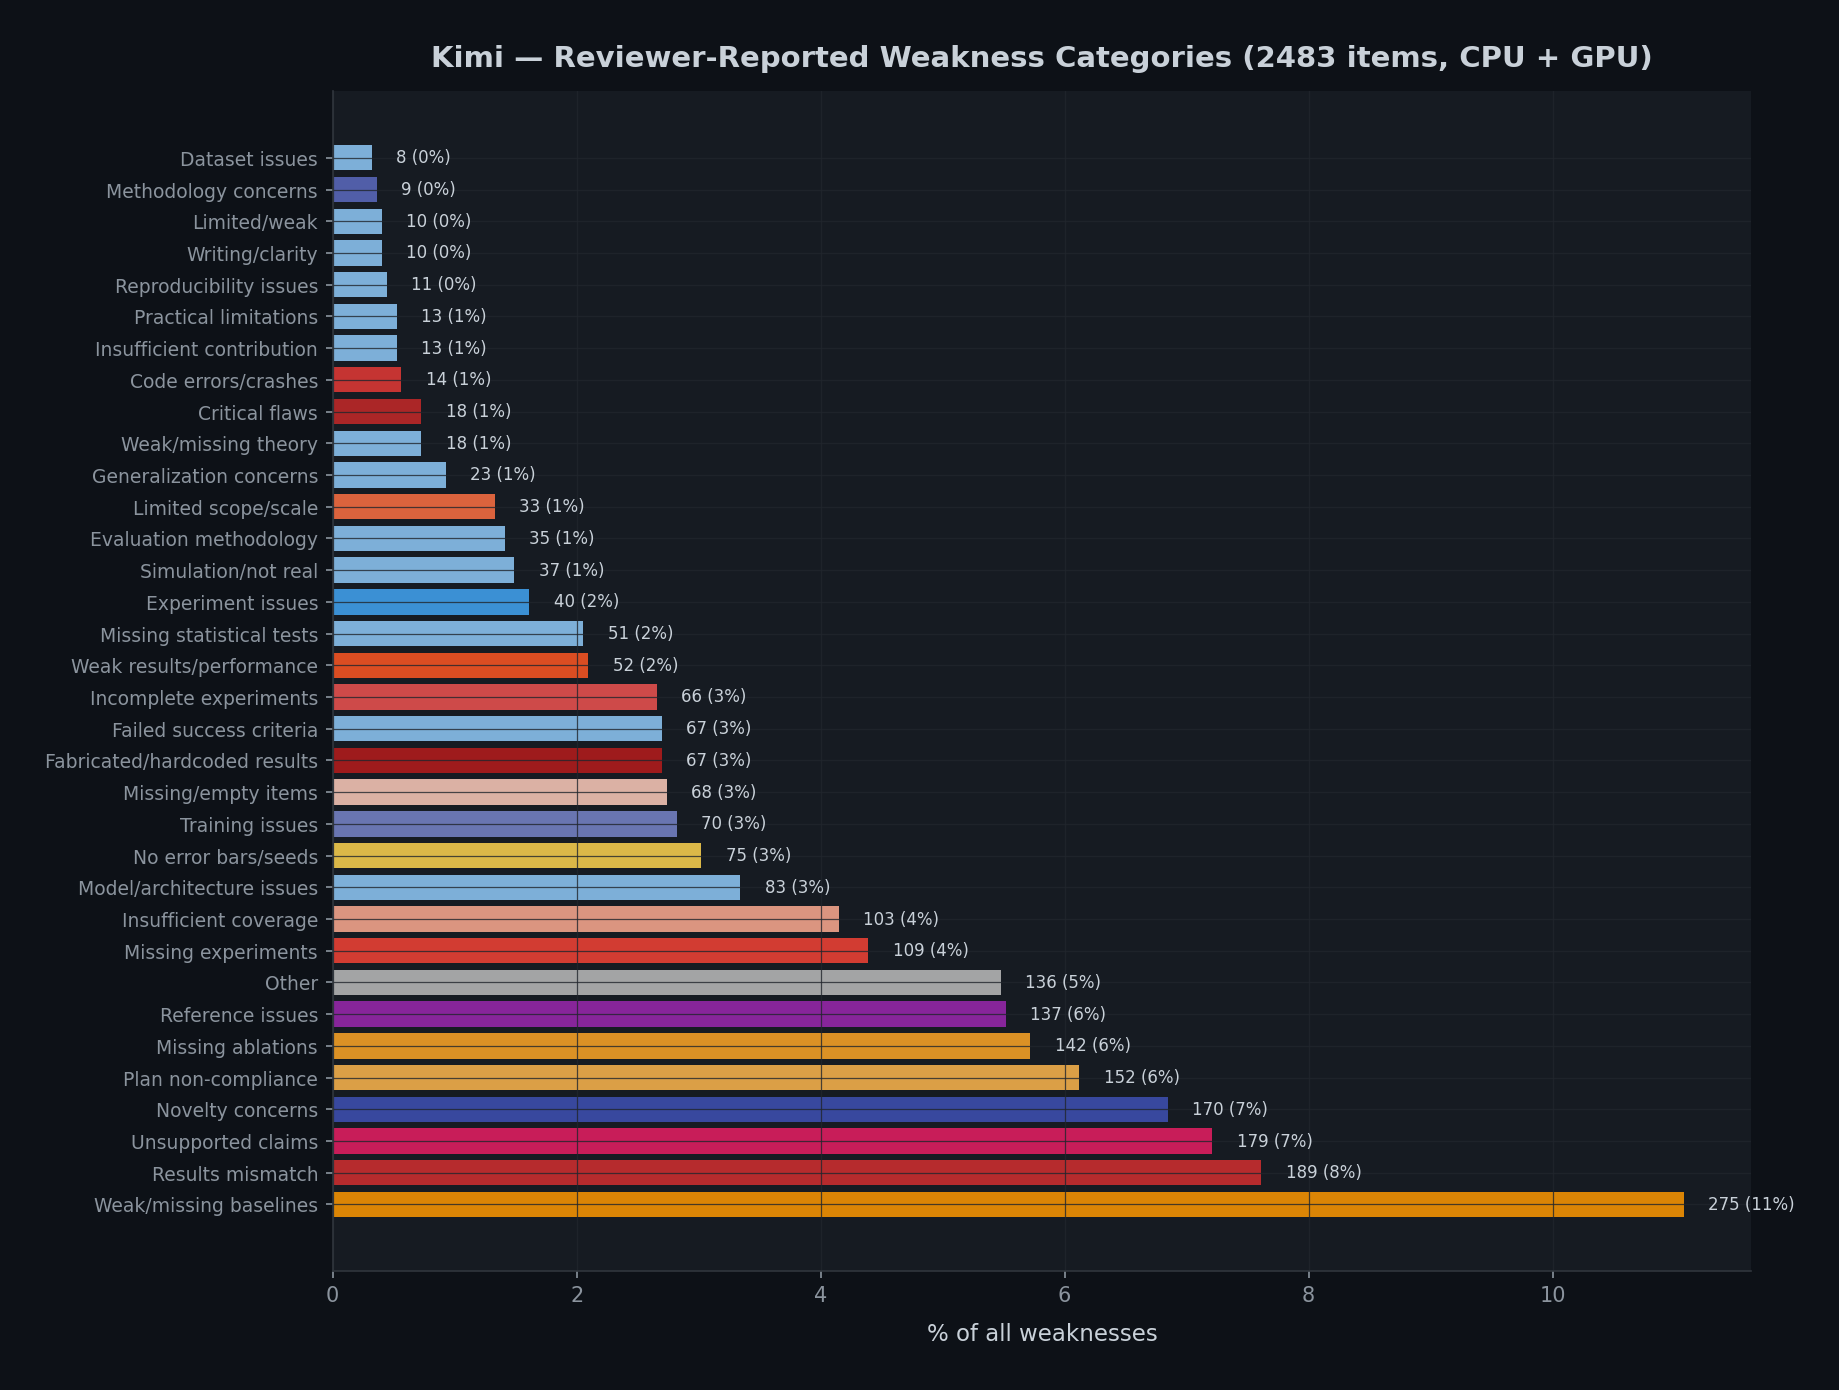
\includegraphics[width=\linewidth]{kimi_failure_categories.png}
\caption{Kimi}
\end{subfigure}
\caption{Failure categories by agent.}
\end{figure}

\subsection{Language Use and Experiment Completion}

\begin{figure}[h]
\centering
\begin{subfigure}{0.32\linewidth}
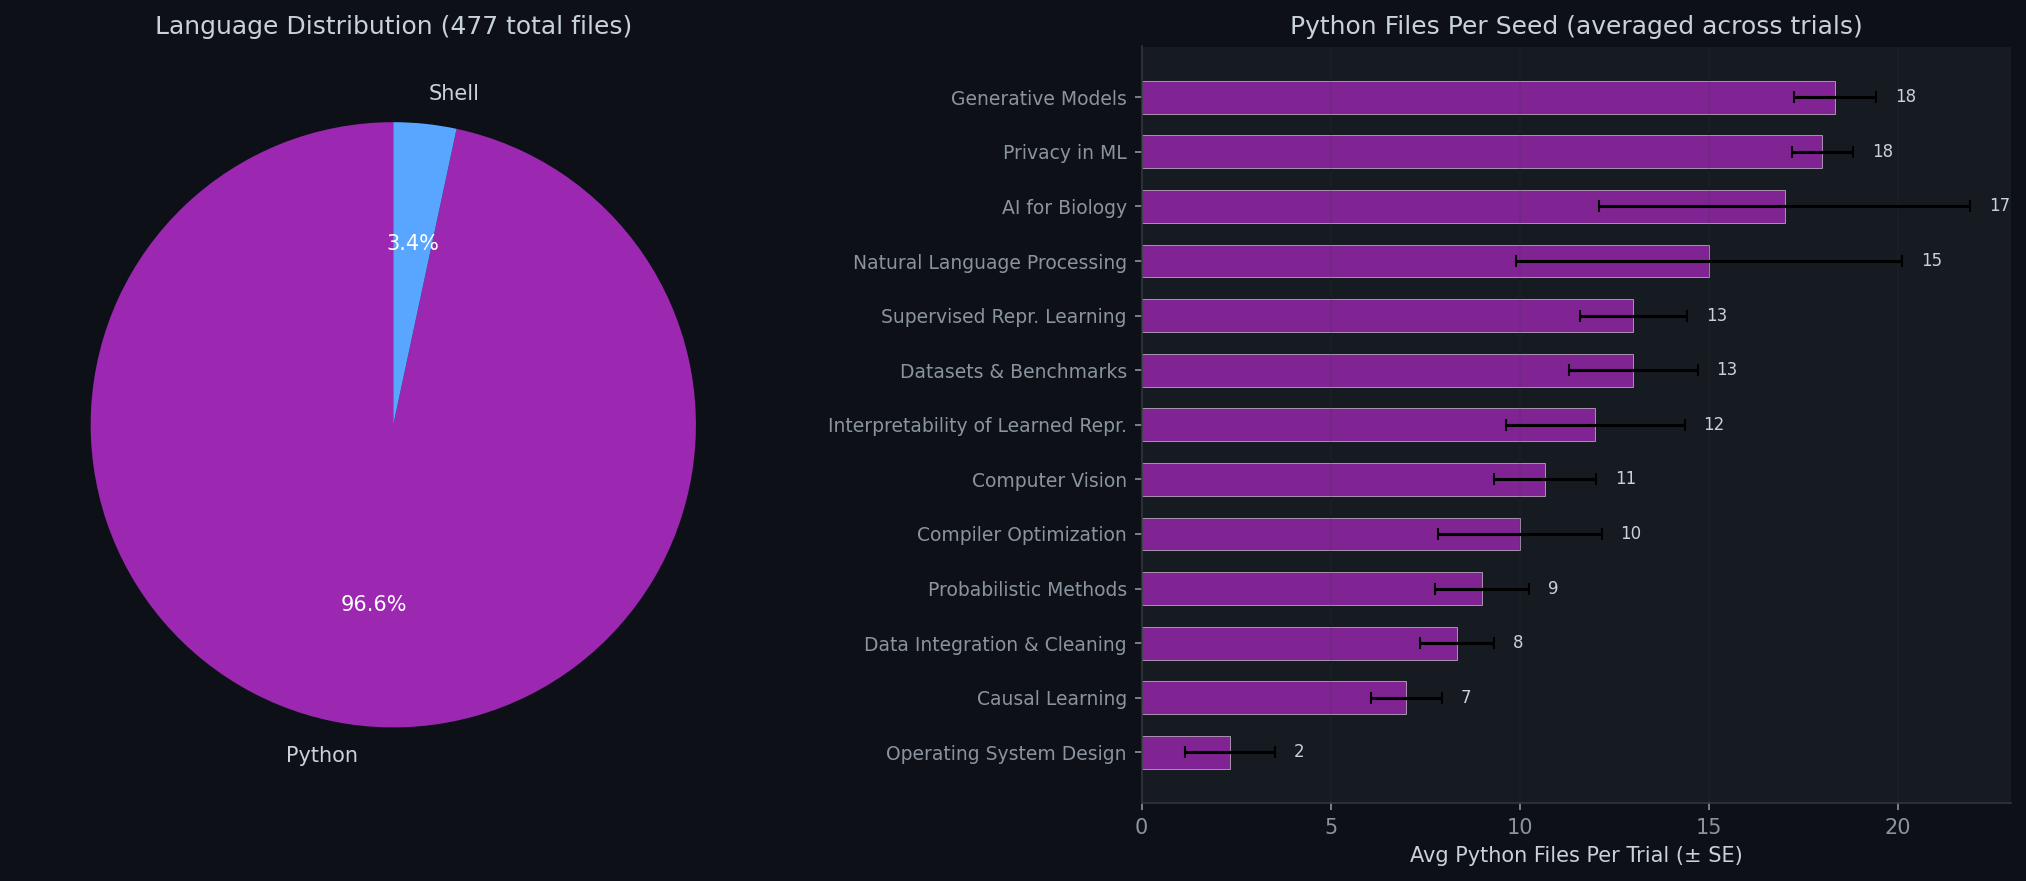
\includegraphics[width=\linewidth]{claude_language_usage.png}
\caption{Claude}
\end{subfigure}
\begin{subfigure}{0.32\linewidth}

\includegraphics[width=\linewidth]{codex_language_usage.png}
\caption{Codex}
\end{subfigure}
\begin{subfigure}{0.32\linewidth}
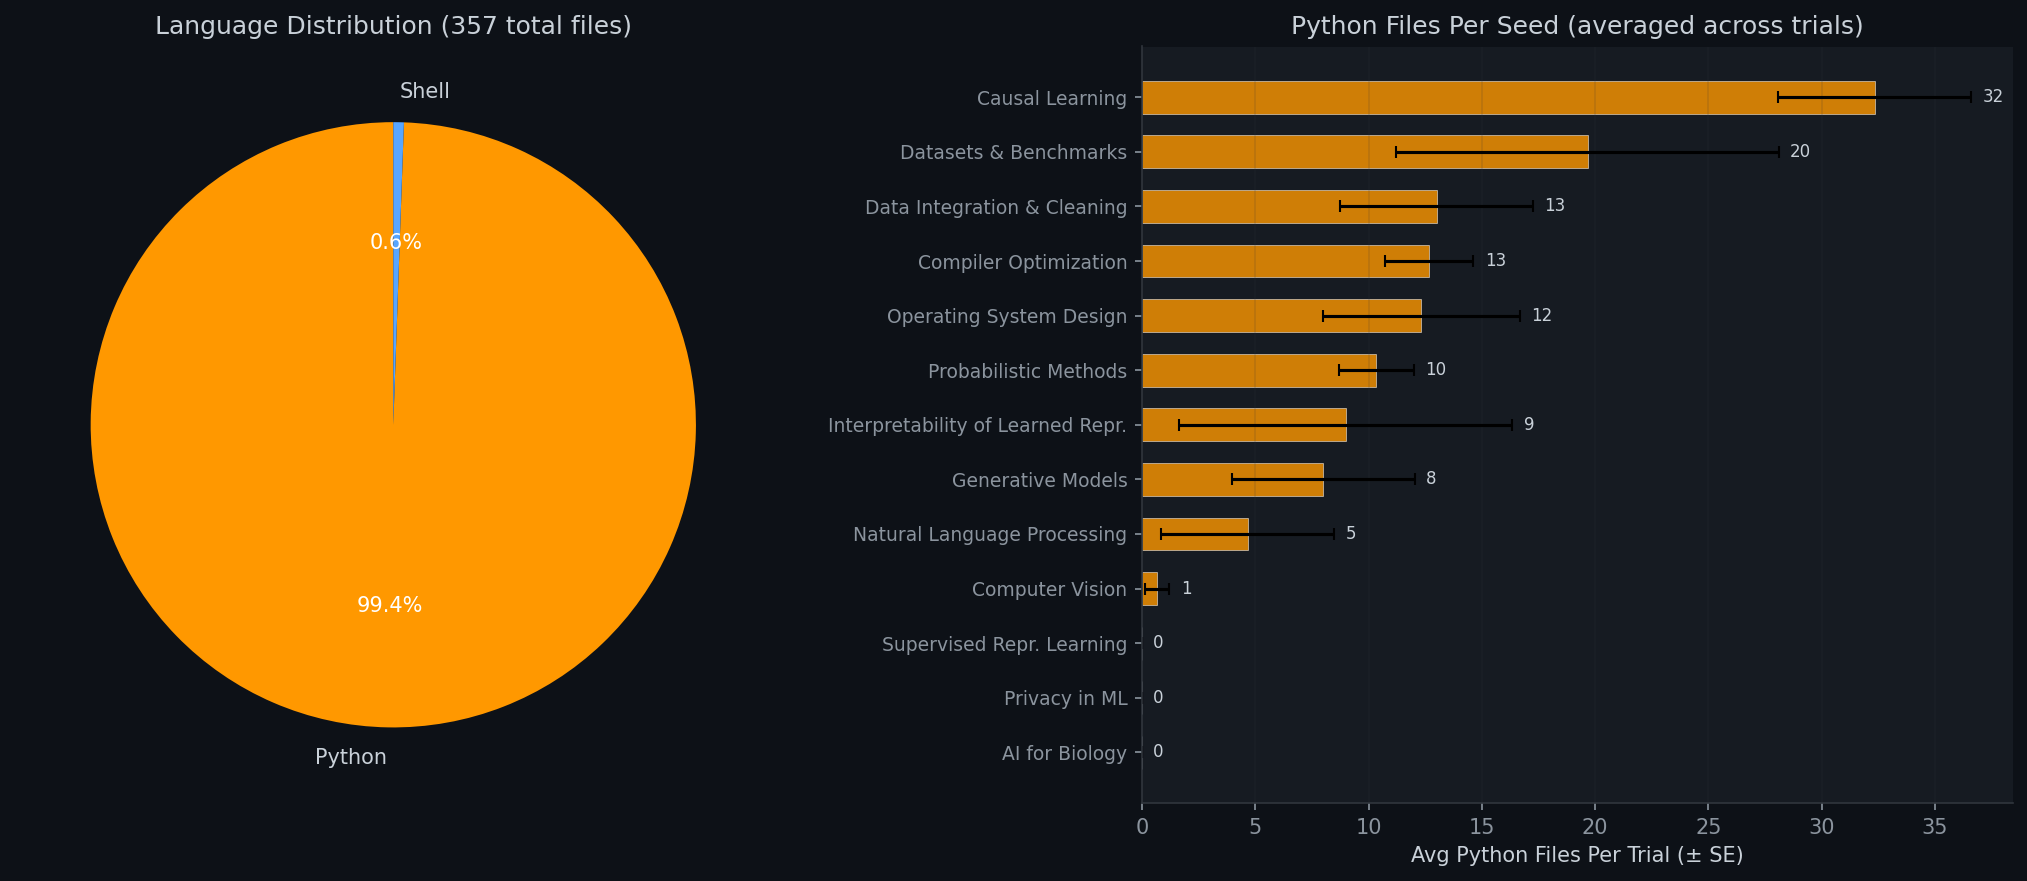
\includegraphics[width=\linewidth]{kimi_language_usage.png}
\caption{Kimi}
\end{subfigure}
\caption{Programming-language usage. All three agents overwhelmingly default to Python.}
\end{figure}

\begin{figure}[h]
\centering
\begin{subfigure}{0.32\linewidth}

\includegraphics[width=\linewidth]{claude_experiment_completion.png}
\caption{Claude}
\end{subfigure}
\begin{subfigure}{0.32\linewidth}

\includegraphics[width=\linewidth]{codex_experiment_completion.png}
\caption{Codex}
\end{subfigure}
\begin{subfigure}{0.32\linewidth}

\includegraphics[width=\linewidth]{kimi_experiment_completion.png}
\caption{Kimi}
\end{subfigure}
\caption{Experiment completion diagnostics.}
\end{figure}

\subsection{Self-Review and Reviewer Bias}

\begin{table}[h]
\centering
\small
\begin{tabular}{lrrrr}
\toprule
Agent/stage & Improved & Same & Declined & Mean change \\
\midrule
Claude/Idea & 100\% & 0\% & 0\% & +2.1 \\
Claude/Experiment & 88\% & 8\% & 4\% & +2.2 \\
Claude/Paper & 43\% & 34\% & 23\% & +0.0 \\
Codex/Idea & 35\% & 51\% & 15\% & +0.4 \\
Codex/Experiment & 78\% & 20\% & 2\% & +2.0 \\
Codex/Paper & 64\% & 29\% & 7\% & +1.5 \\
Kimi/Idea & 100\% & 0\% & 0\% & +3.0 \\
Kimi/Experiment & 91\% & 9\% & 0\% & +2.2 \\
Kimi/Paper & 61\% & 34\% & 5\% & +1.6 \\
\bottomrule
\end{tabular}
\caption{Self-review impact by stage. Self-review helps ideation and experiments more consistently than final paper quality, which remains constrained by the underlying idea and evidence.}
\end{table}

\begin{table}[h]
\centering
\small
\begin{tabular}{lrrrr}
\toprule
Reviewer / paper agent & Claude & Codex & Kimi & Avg. given \\
\midrule
Claude Code & 4.6 & 4.0 & 3.2 & 3.9 \\
Codex & 2.9 & 3.9 & 1.9 & 2.9 \\
Kimi Code & 6.2 & 5.7 & 5.0 & 5.7 \\
\bottomrule
\end{tabular}
\caption{Reviewer severity table. Codex is strictest and Kimi Code most lenient.}
\end{table}

\begin{figure}[h]
\centering
\begin{subfigure}{0.32\linewidth}
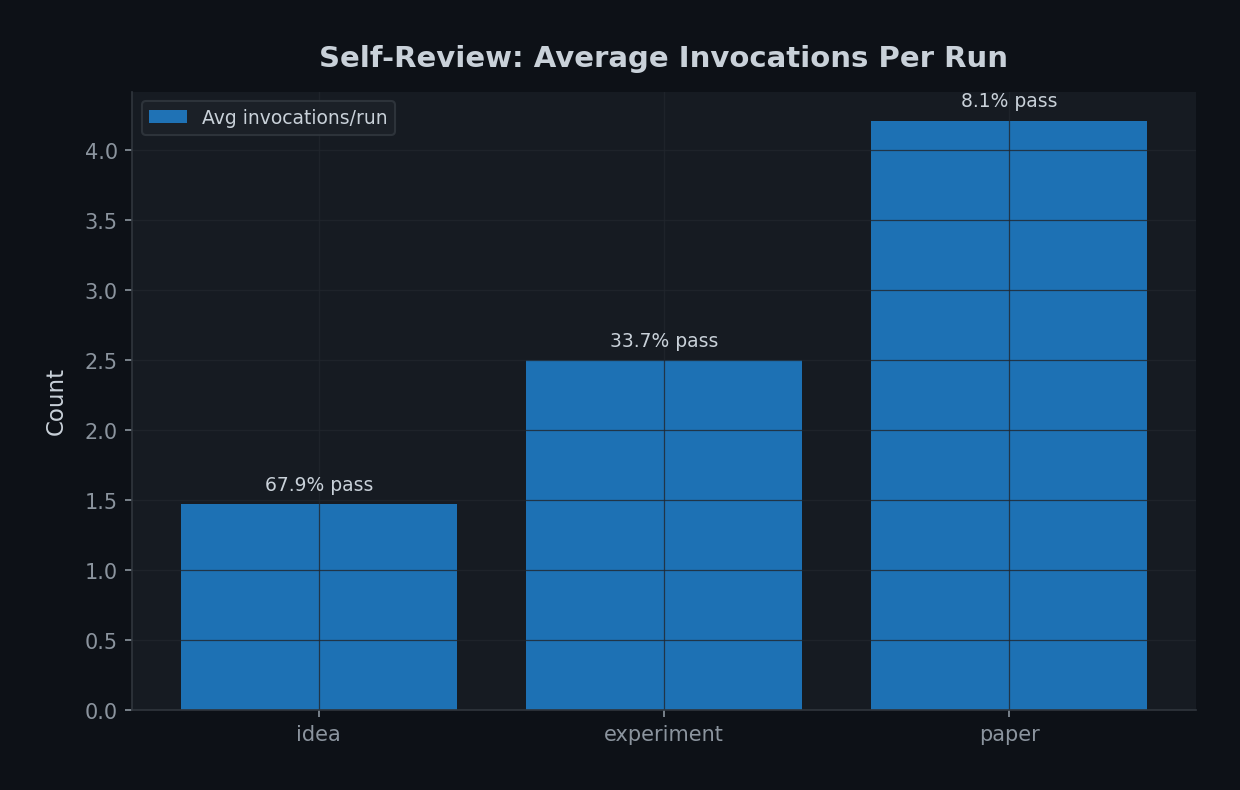
\includegraphics[width=\linewidth]{claude_self_review_impact.png}
\caption{Claude}
\end{subfigure}
\begin{subfigure}{0.32\linewidth}
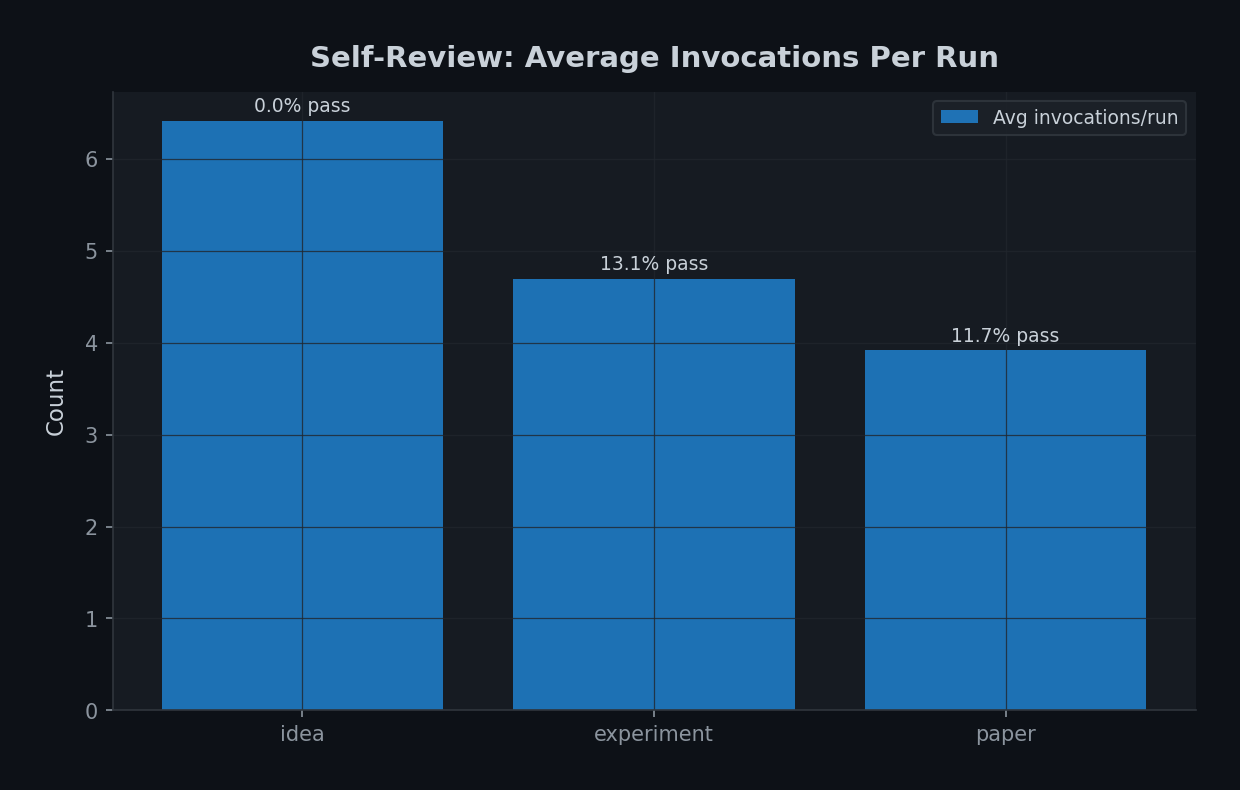
\includegraphics[width=\linewidth]{codex_self_review_impact.png}
\caption{Codex}
\end{subfigure}
\begin{subfigure}{0.32\linewidth}
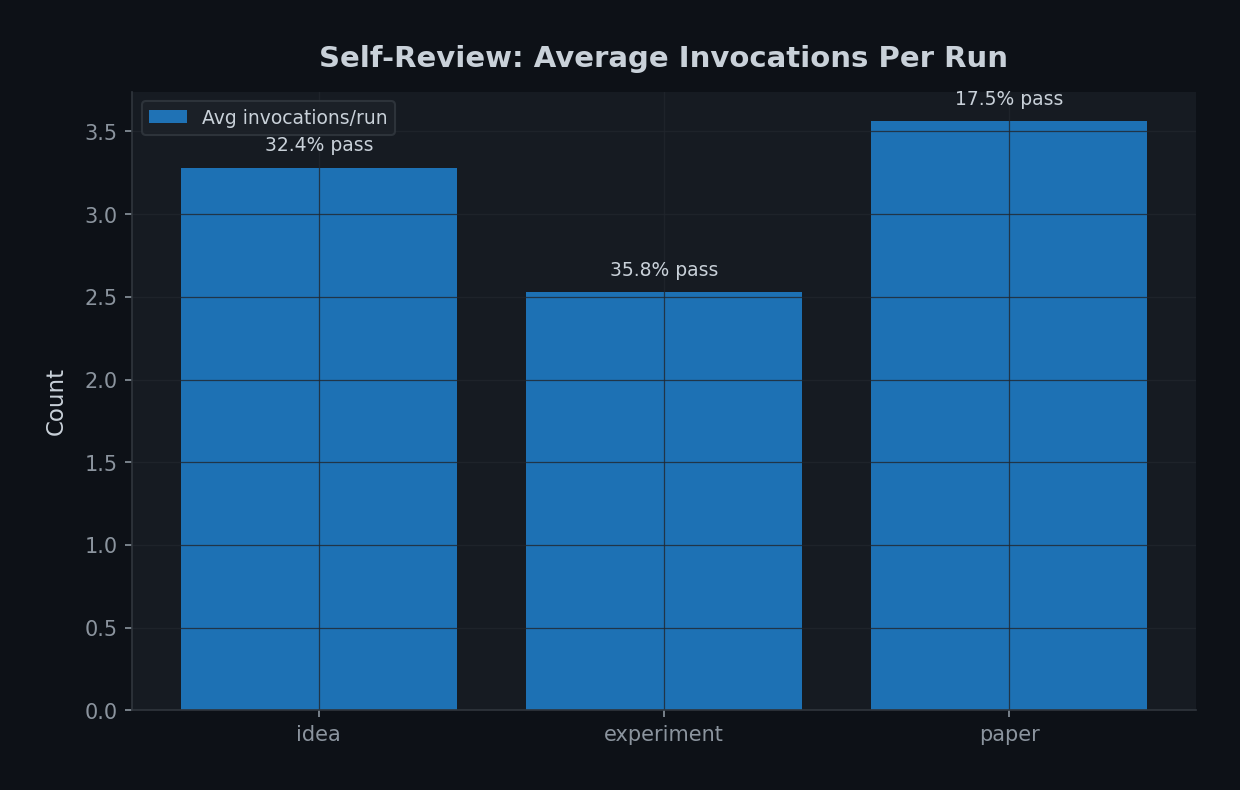
\includegraphics[width=\linewidth]{kimi_self_review_impact.png}
\caption{Kimi}
\end{subfigure}
\caption{Self-review impact plots.}
\end{figure}

\begin{figure}[h]
\centering
\begin{subfigure}{0.32\linewidth}
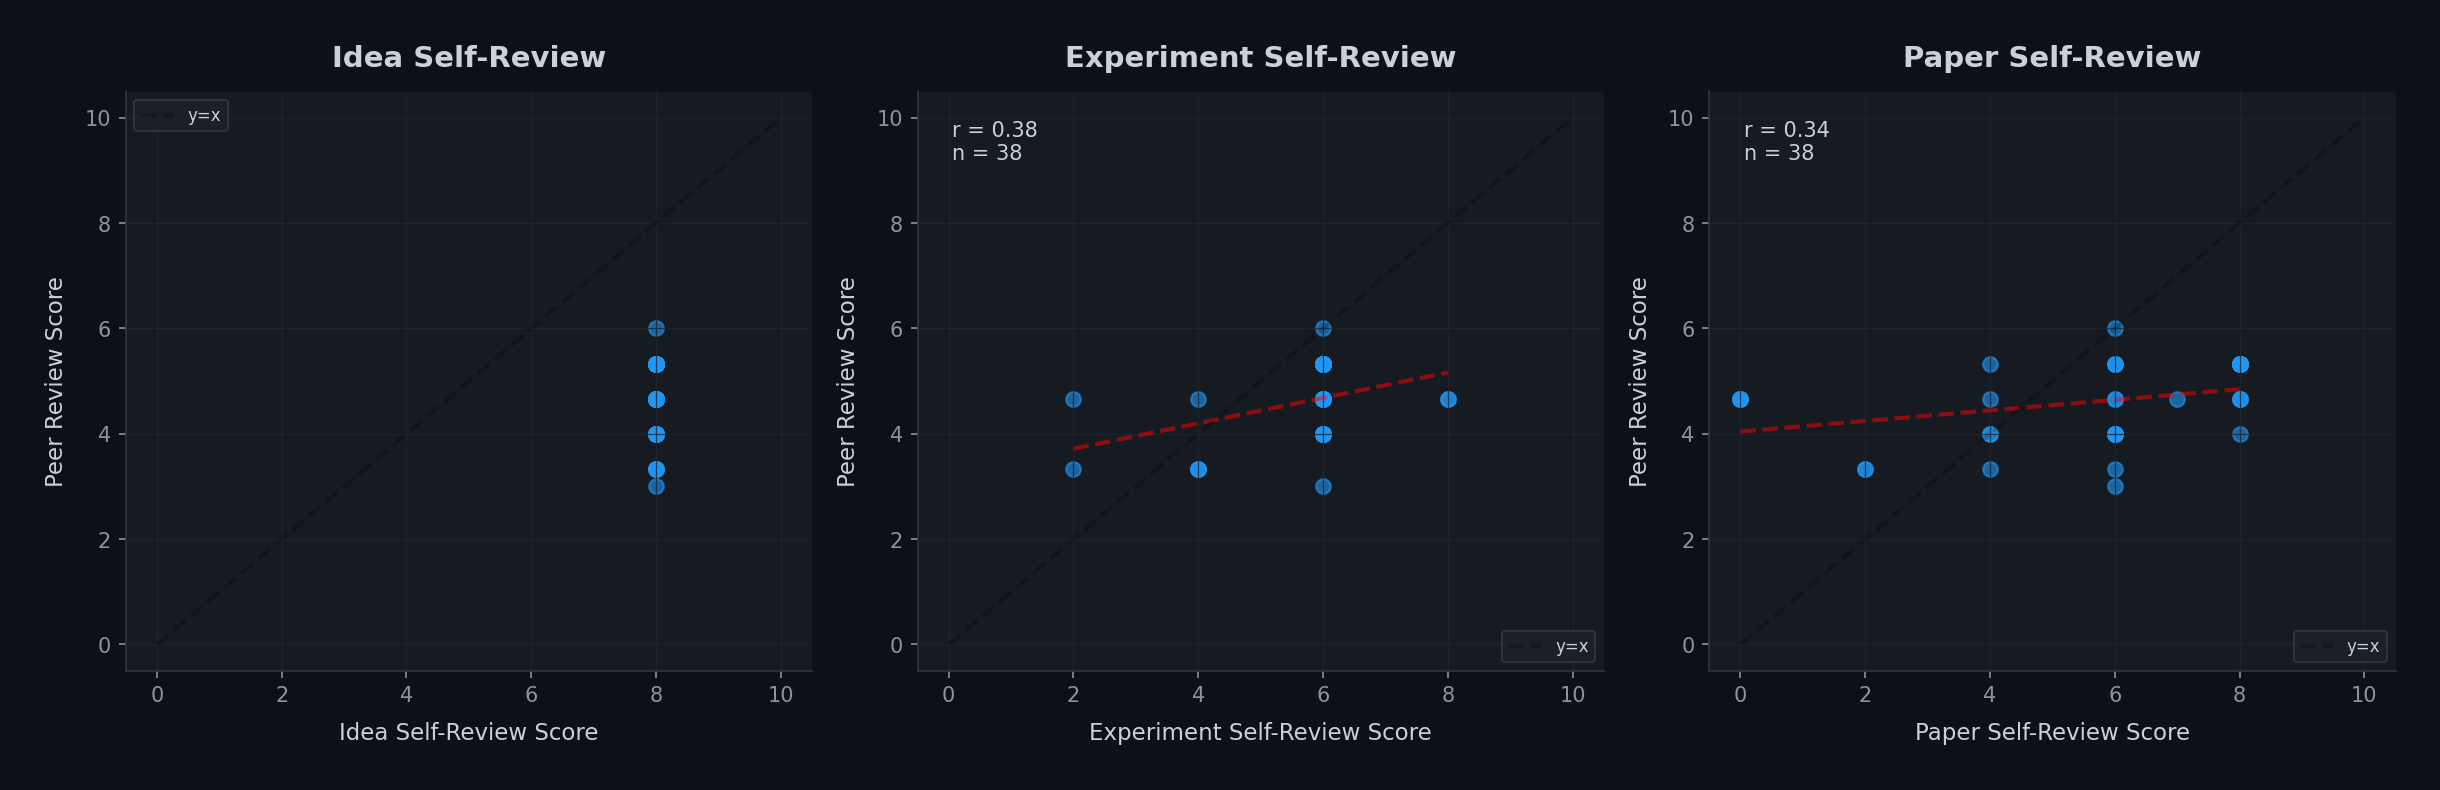
\includegraphics[width=\linewidth]{claude_selfrev_vs_peer.png}
\caption{Claude}
\end{subfigure}
\begin{subfigure}{0.32\linewidth}
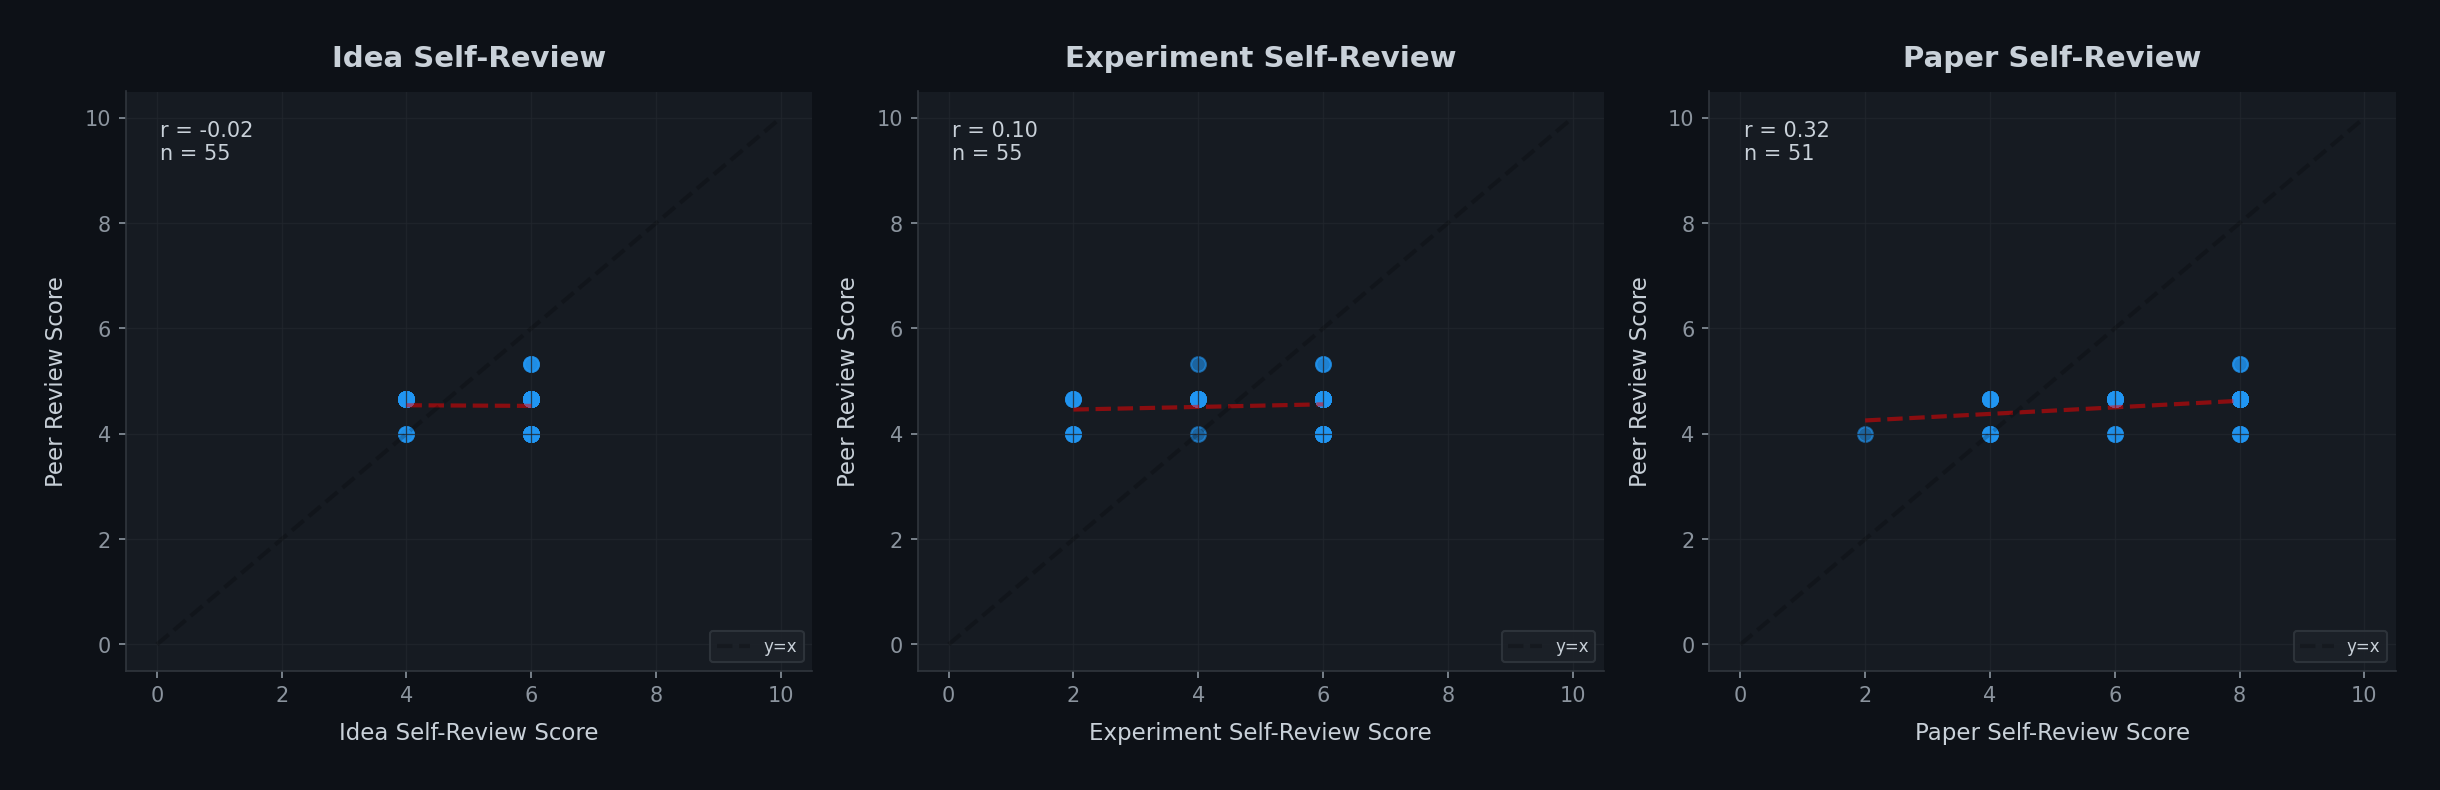
\includegraphics[width=\linewidth]{codex_selfrev_vs_peer.png}
\caption{Codex}
\end{subfigure}
\begin{subfigure}{0.32\linewidth}
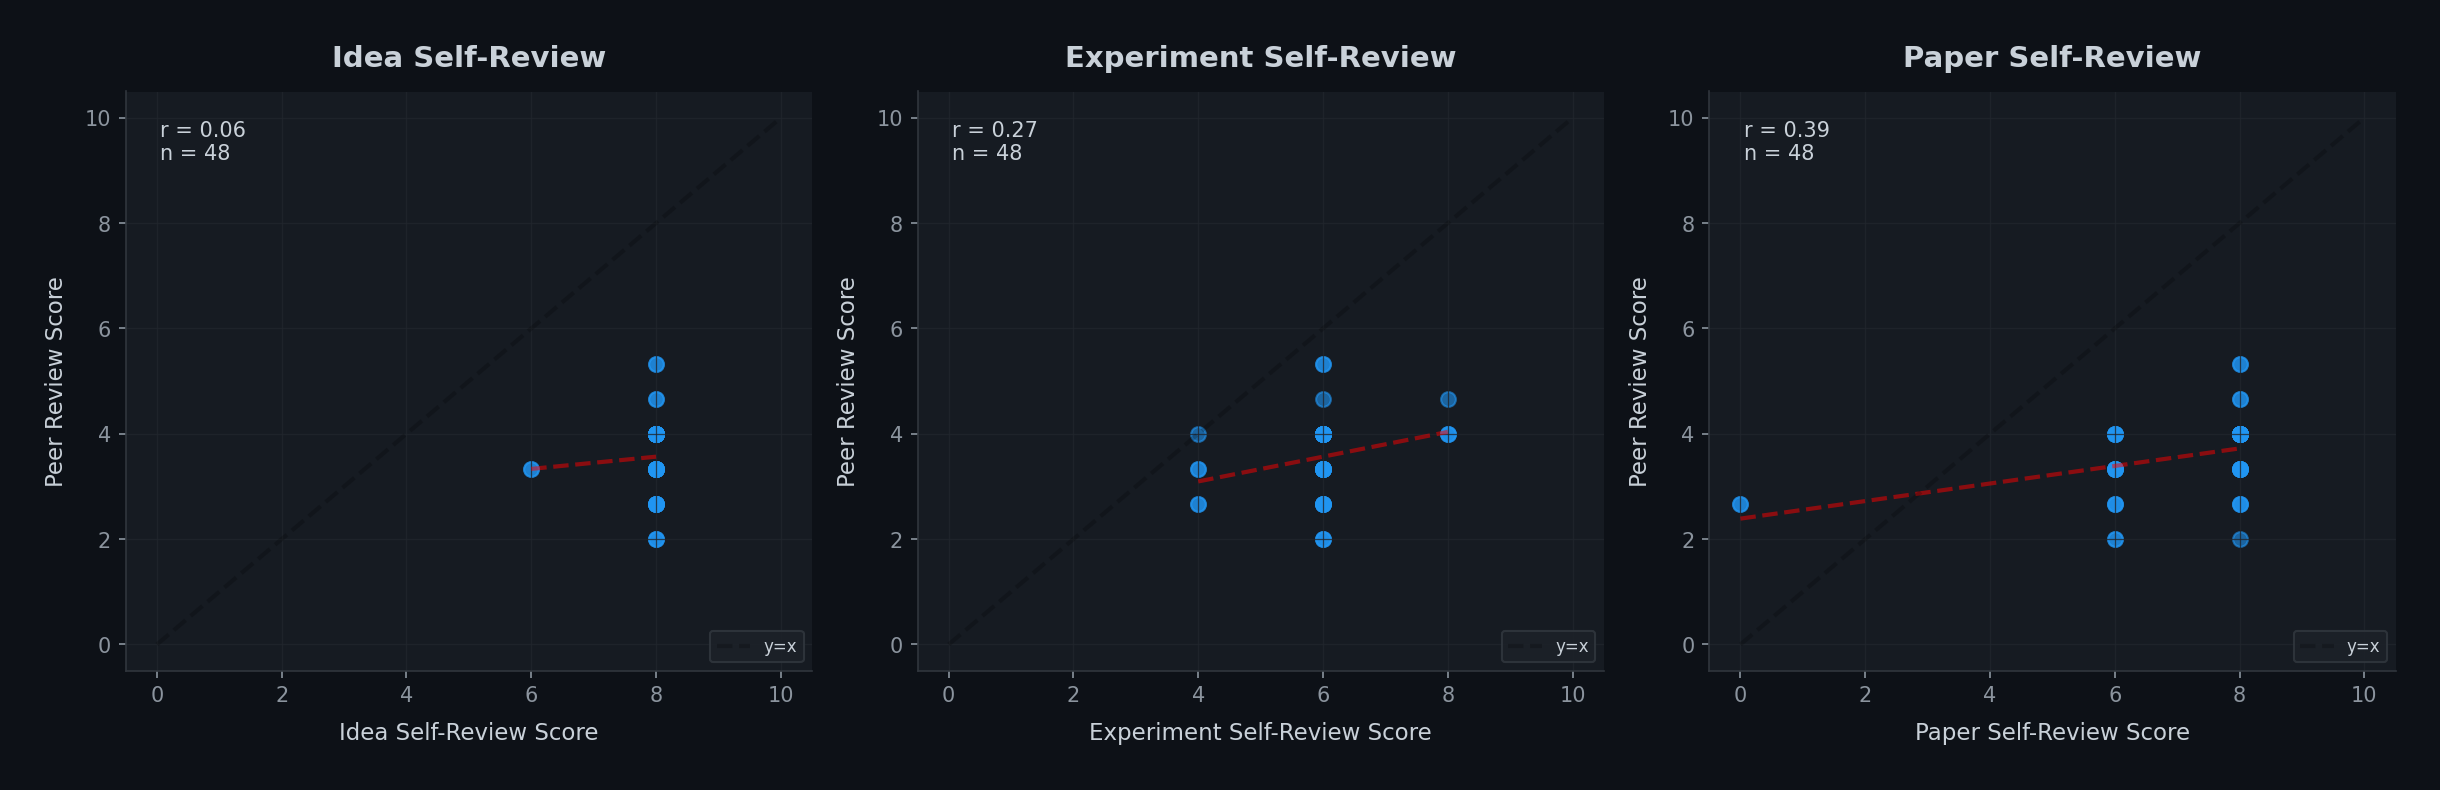
\includegraphics[width=\linewidth]{kimi_selfrev_vs_peer.png}
\caption{Kimi}
\end{subfigure}
\caption{Self-review versus peer-review scores.}
\end{figure}

\begin{figure}[h]
\centering
\begin{subfigure}{0.48\linewidth}
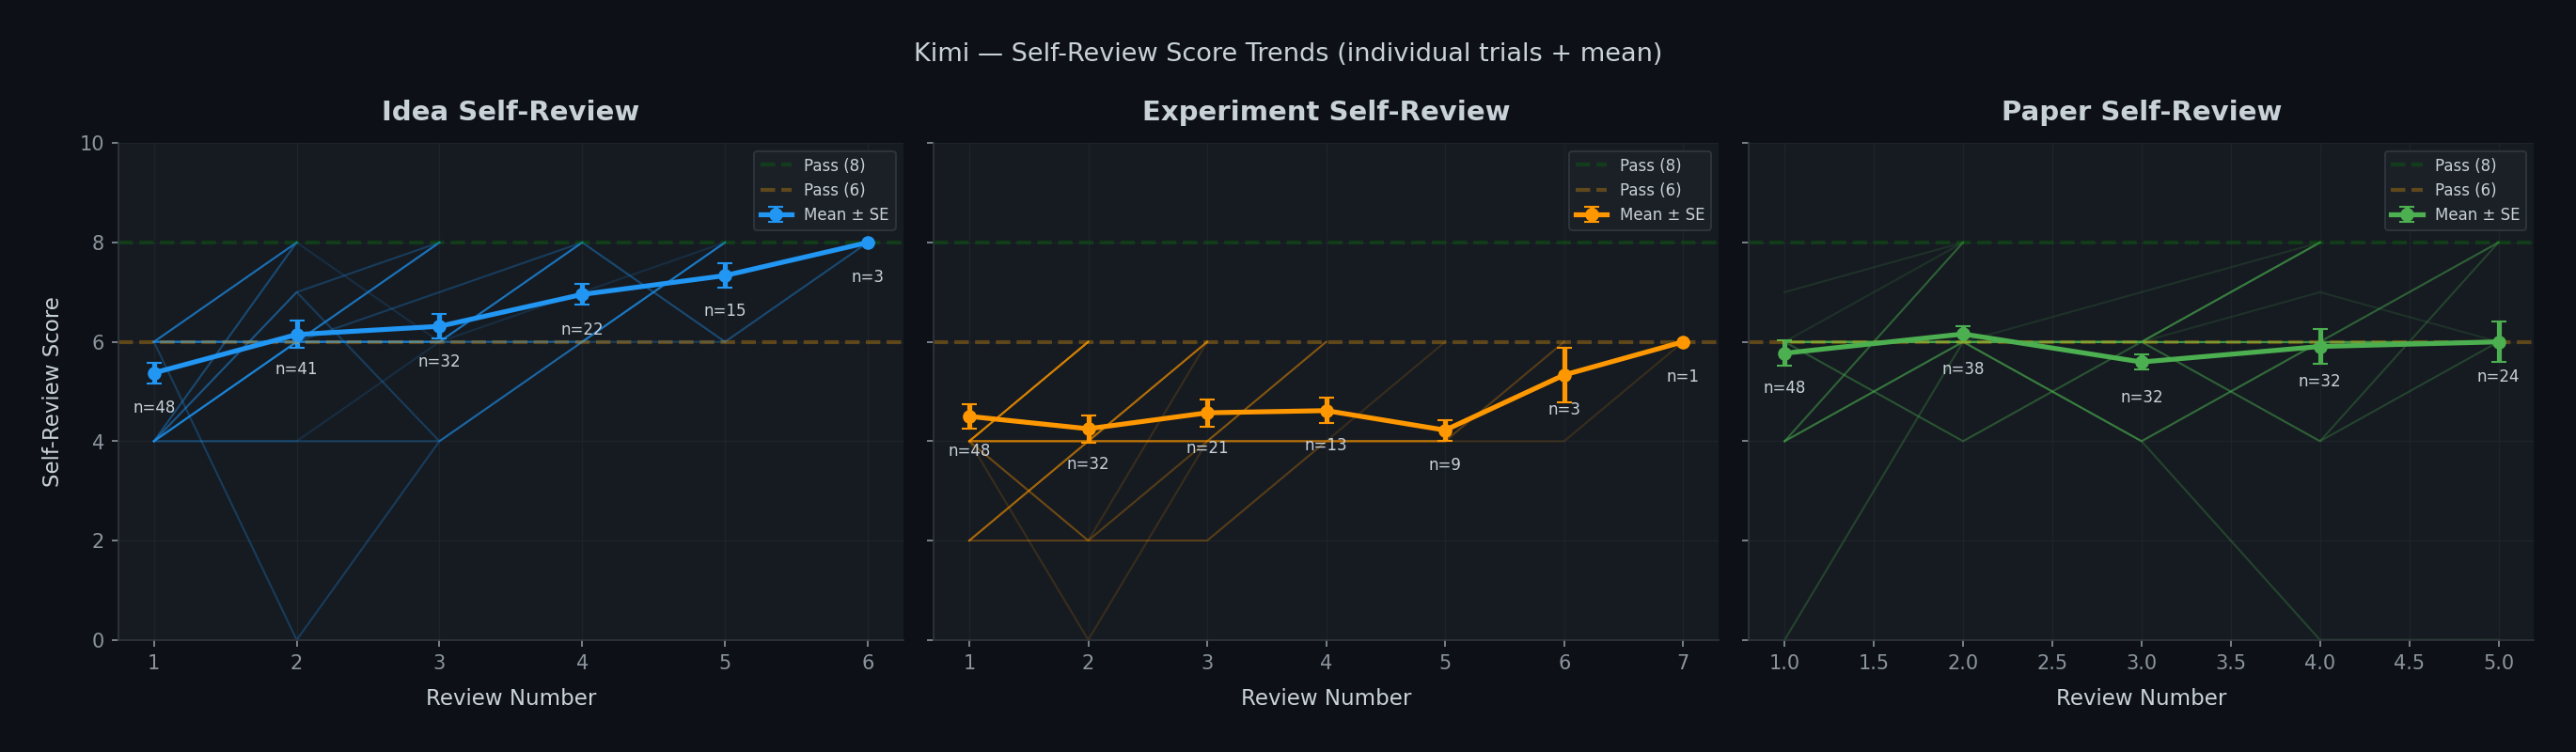
\includegraphics[width=\linewidth]{kimi_self_review_trends.png}
\caption{Kimi self-review trends}
\end{subfigure}
\hfill
\begin{subfigure}{0.48\linewidth}
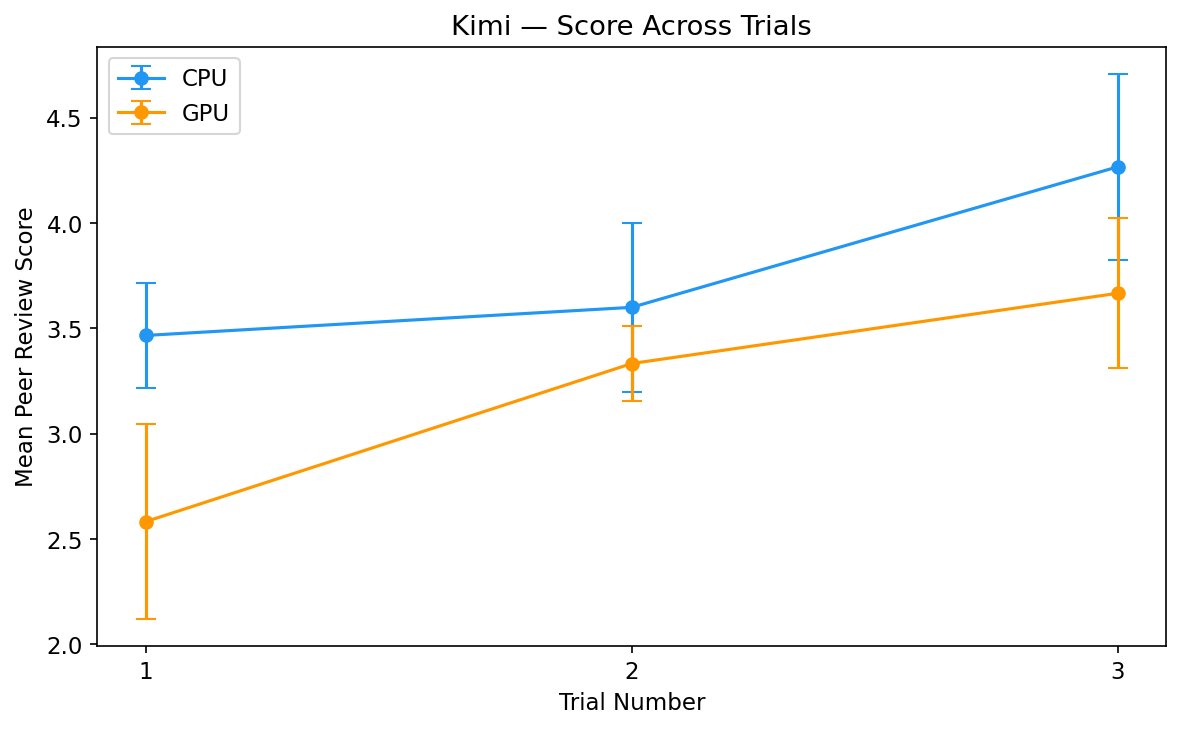
\includegraphics[width=\linewidth]{kimi_trial_improvement.png}
\caption{Kimi trial improvement}
\end{subfigure}
\caption{Additional Kimi self-review diagnostics.}
\end{figure}

\begin{figure}[h]
\centering
\begin{subfigure}{0.32\linewidth}
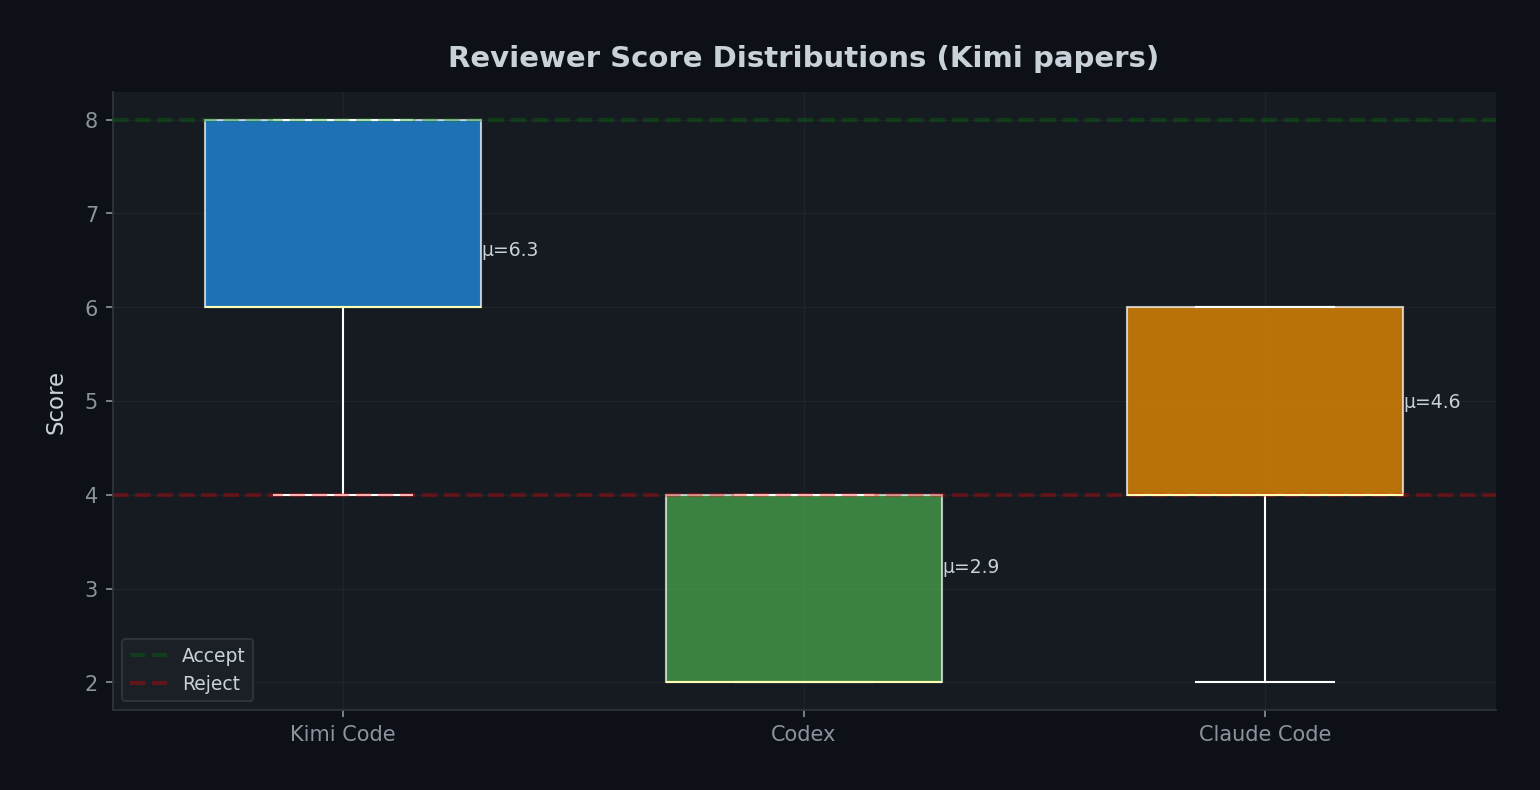
\includegraphics[width=\linewidth]{claude_reviewer_bias.png}
\caption{Claude}
\end{subfigure}
\begin{subfigure}{0.32\linewidth}
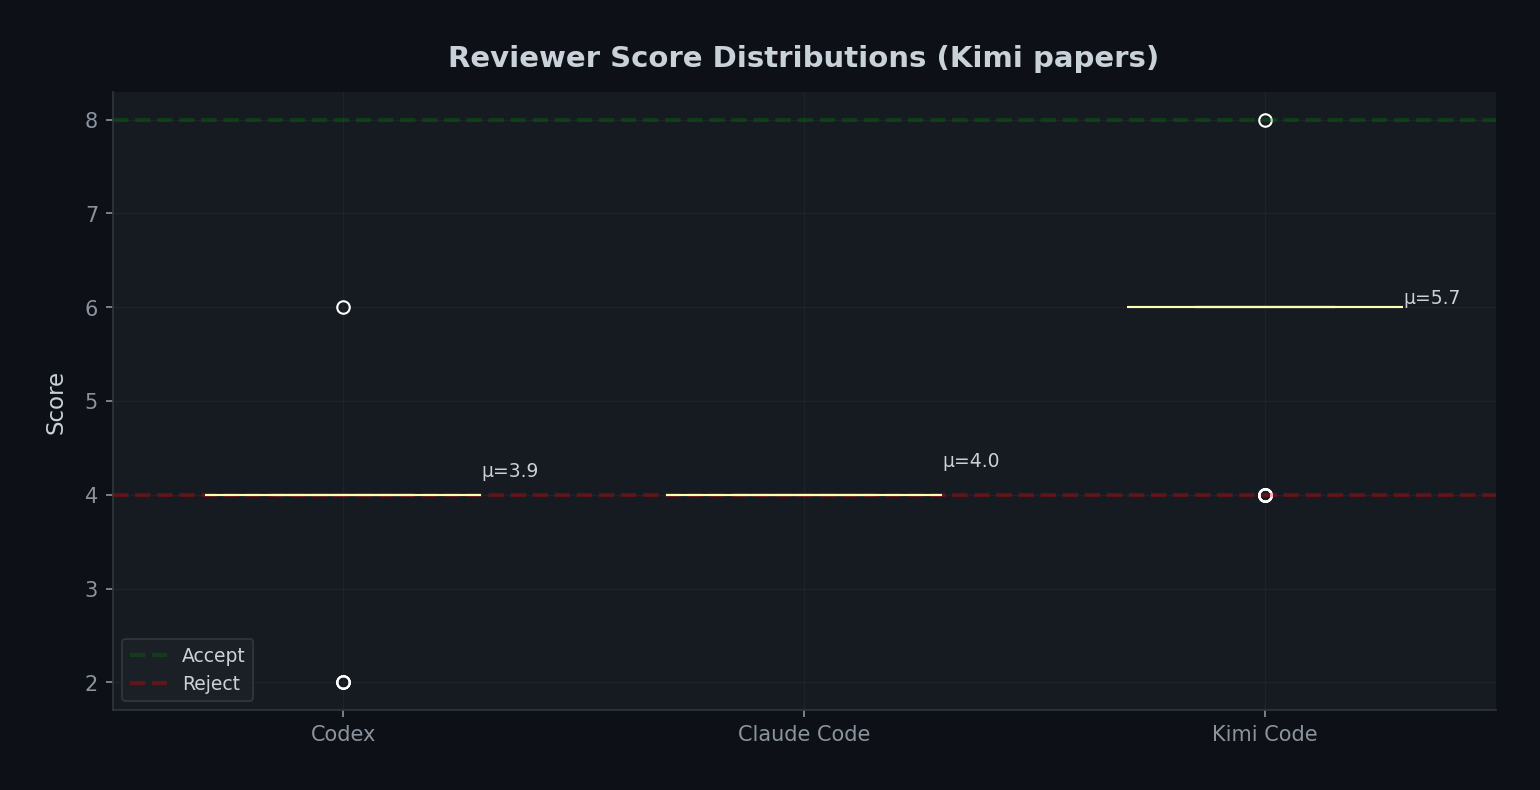
\includegraphics[width=\linewidth]{codex_reviewer_bias.png}
\caption{Codex}
\end{subfigure}
\begin{subfigure}{0.32\linewidth}
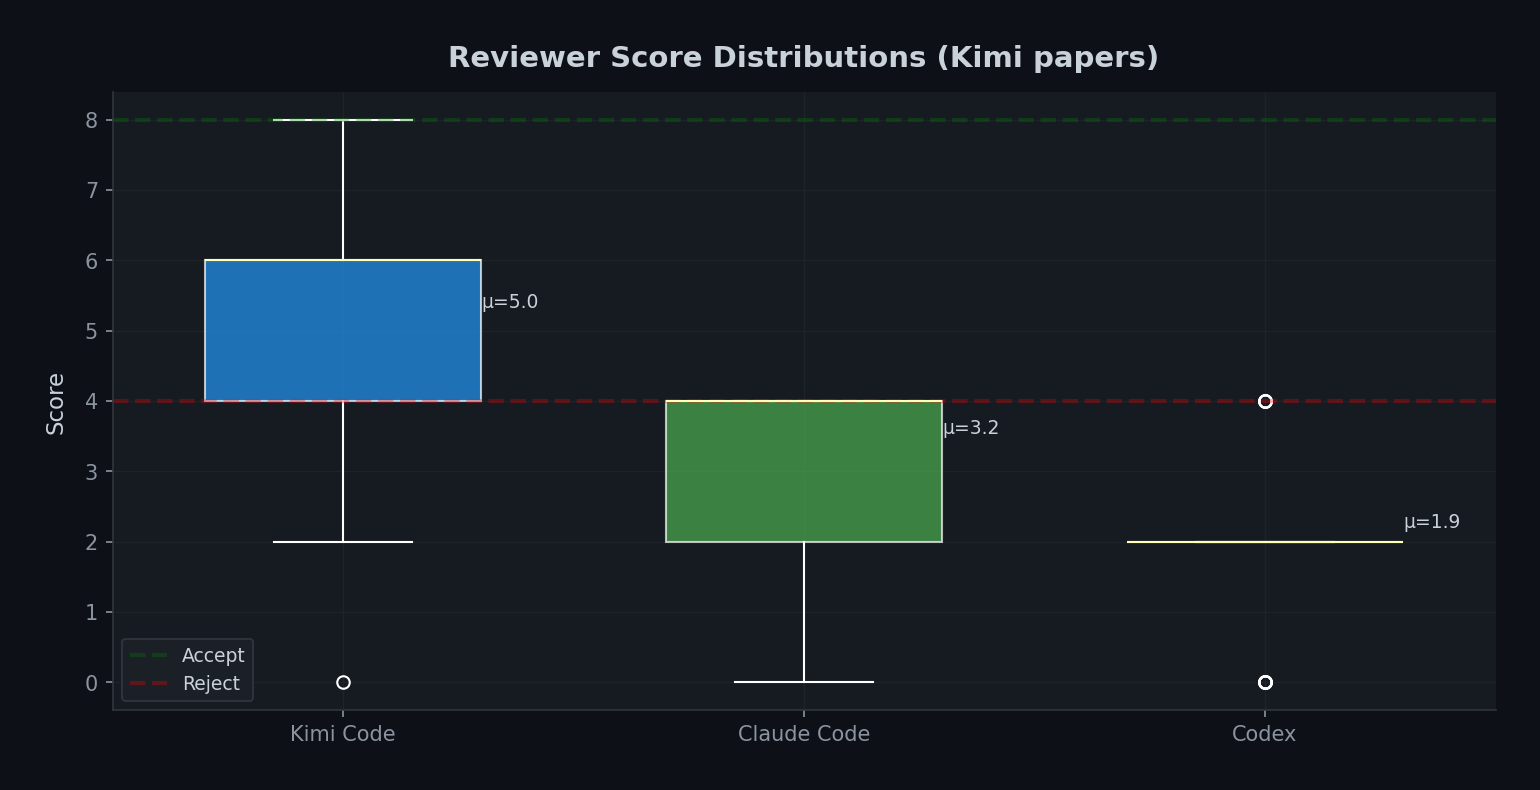
\includegraphics[width=\linewidth]{kimi_reviewer_bias.png}
\caption{Kimi}
\end{subfigure}
\caption{Reviewer-bias diagnostics.}
\end{figure}

\begin{figure}[h]
\centering
\begin{subfigure}{0.32\linewidth}
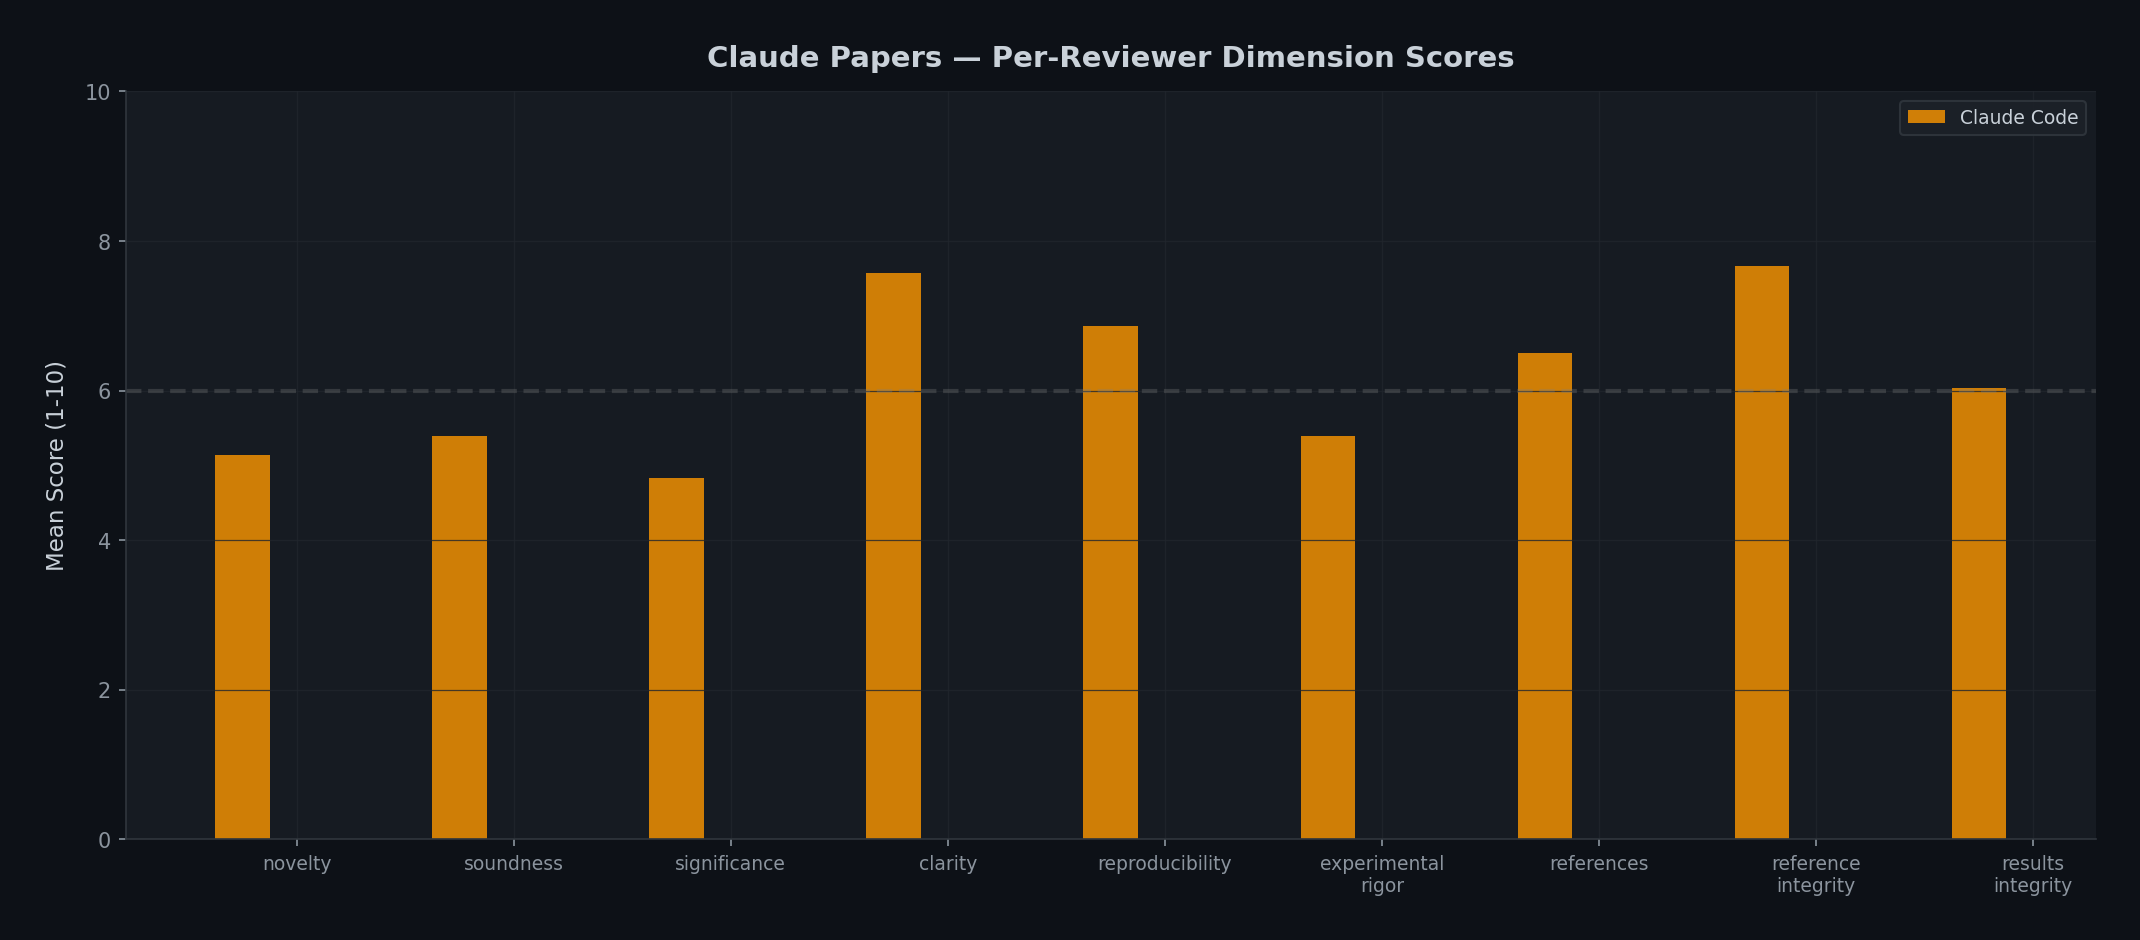
\includegraphics[width=\linewidth]{claude_reviewer_dimensions.png}
\caption{Claude}
\end{subfigure}
\begin{subfigure}{0.32\linewidth}
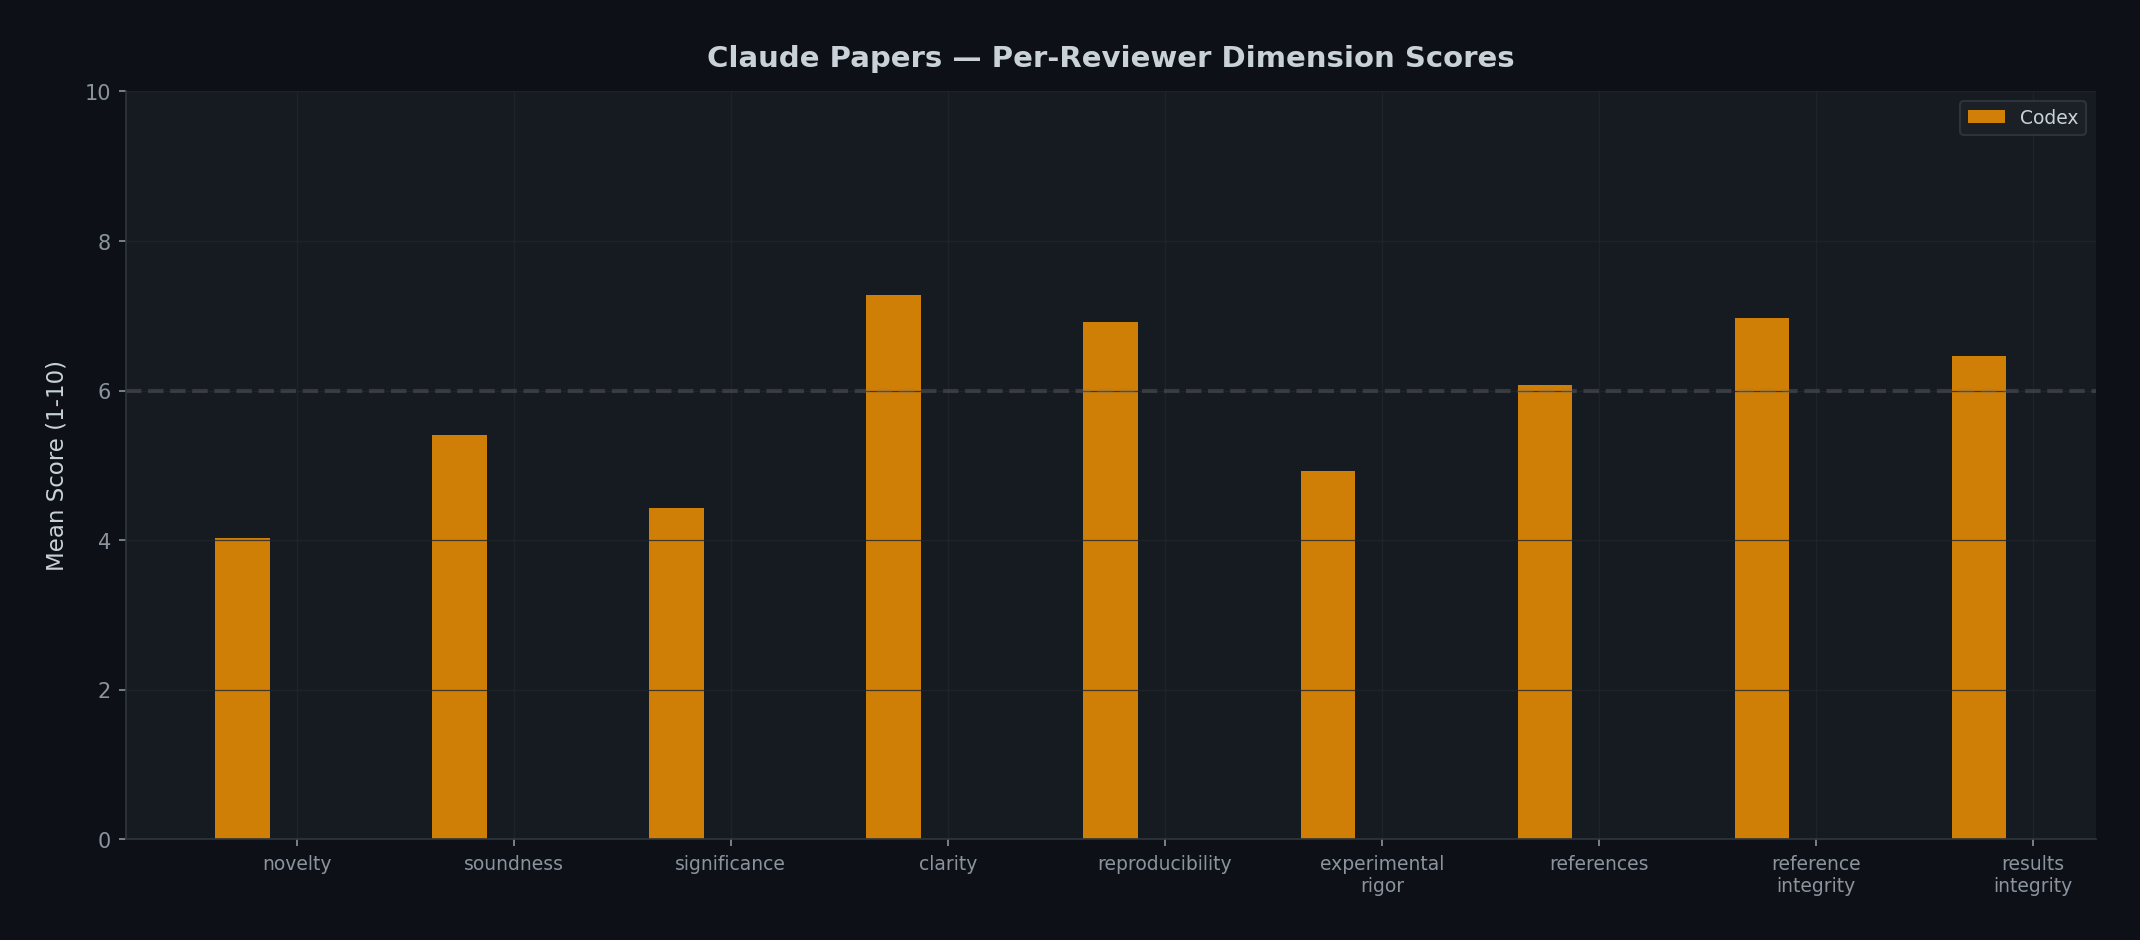
\includegraphics[width=\linewidth]{codex_reviewer_dimensions.png}
\caption{Codex}
\end{subfigure}
\begin{subfigure}{0.32\linewidth}
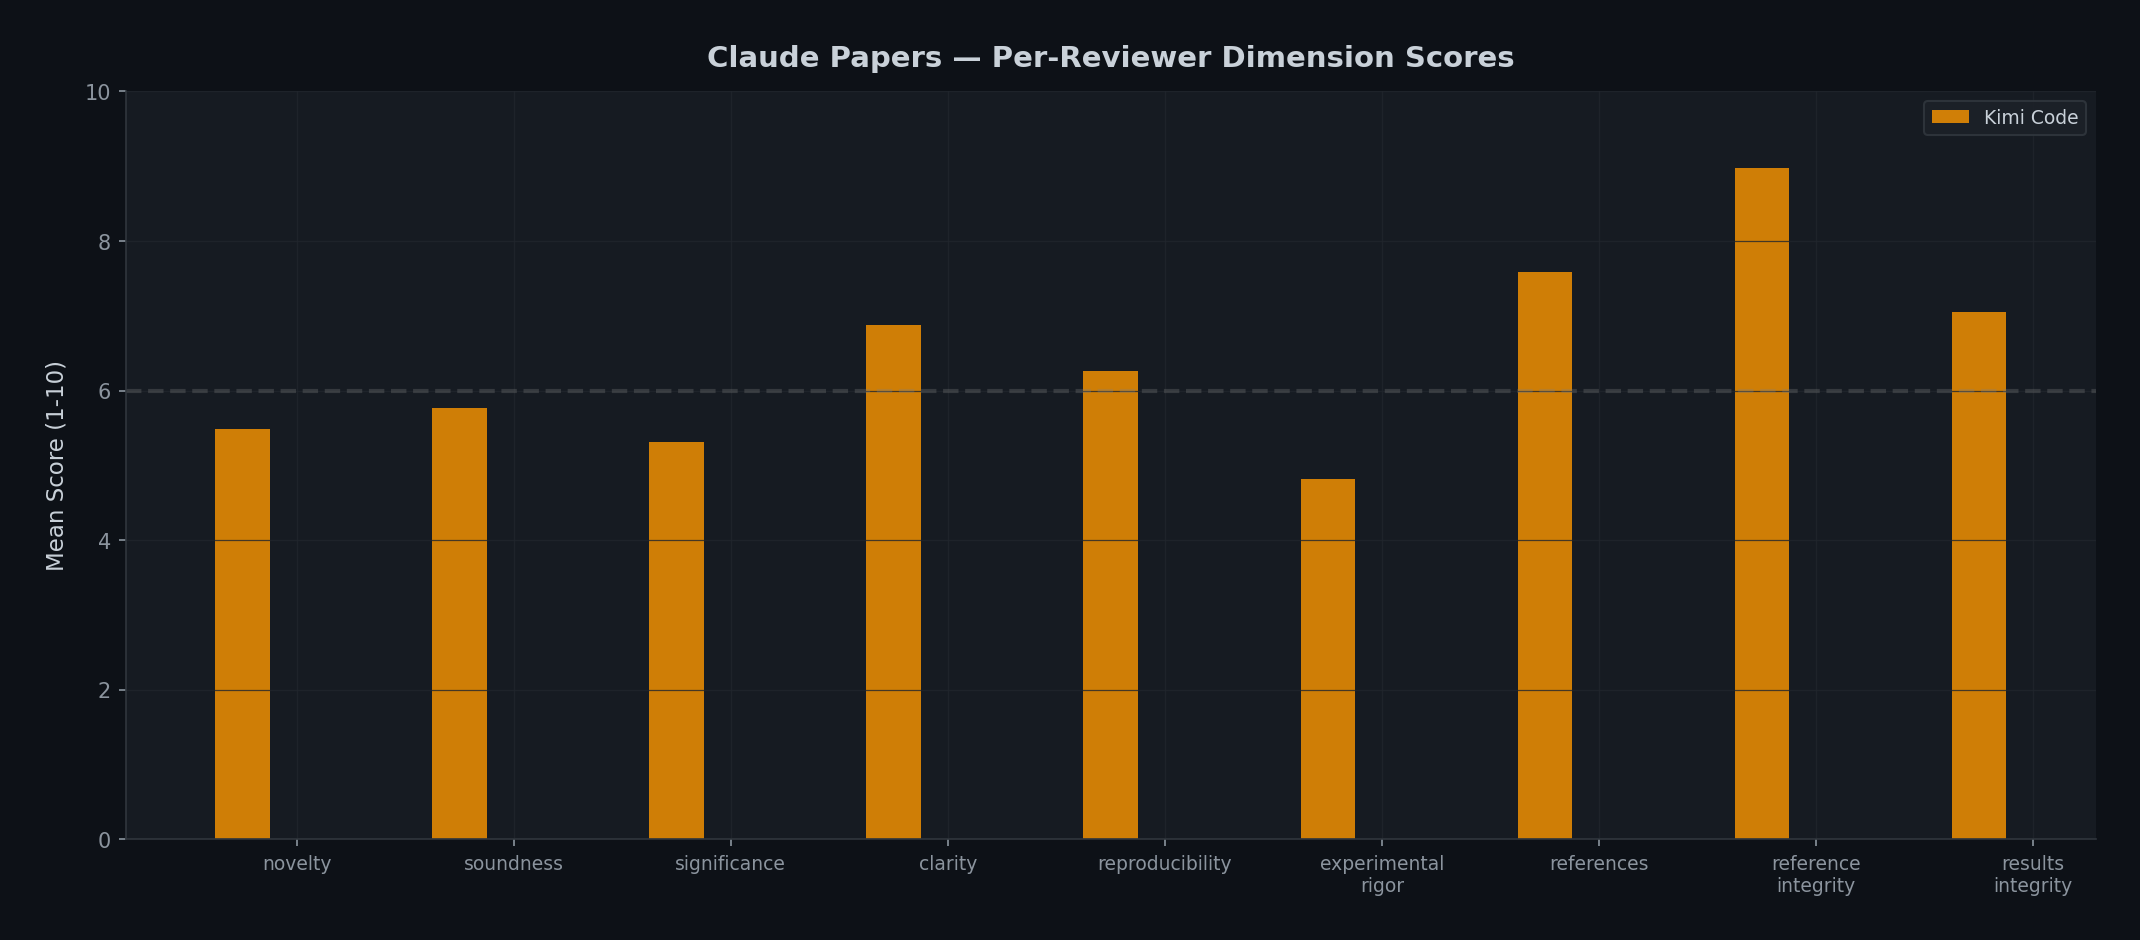
\includegraphics[width=\linewidth]{kimi_reviewer_dimensions.png}
\caption{Kimi}
\end{subfigure}
\caption{Reviewer dimension diagnostics.}
\end{figure}

\subsection{Time and Hardware Diagnostics}

\begin{figure}[h]
\centering
\begin{subfigure}{0.32\linewidth}
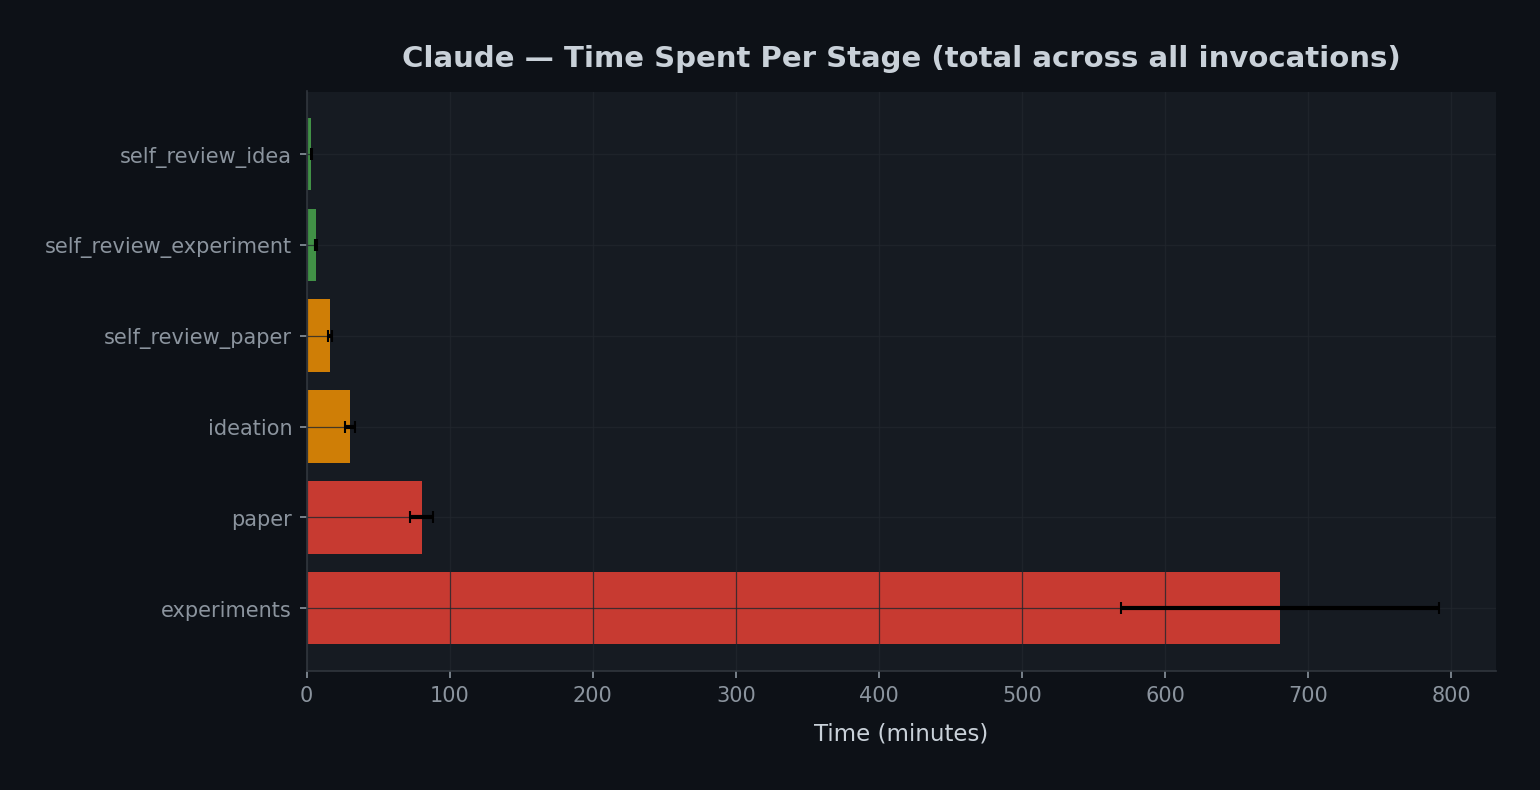
\includegraphics[width=\linewidth]{claude_time_per_stage.png}
\caption{Claude}
\end{subfigure}
\begin{subfigure}{0.32\linewidth}
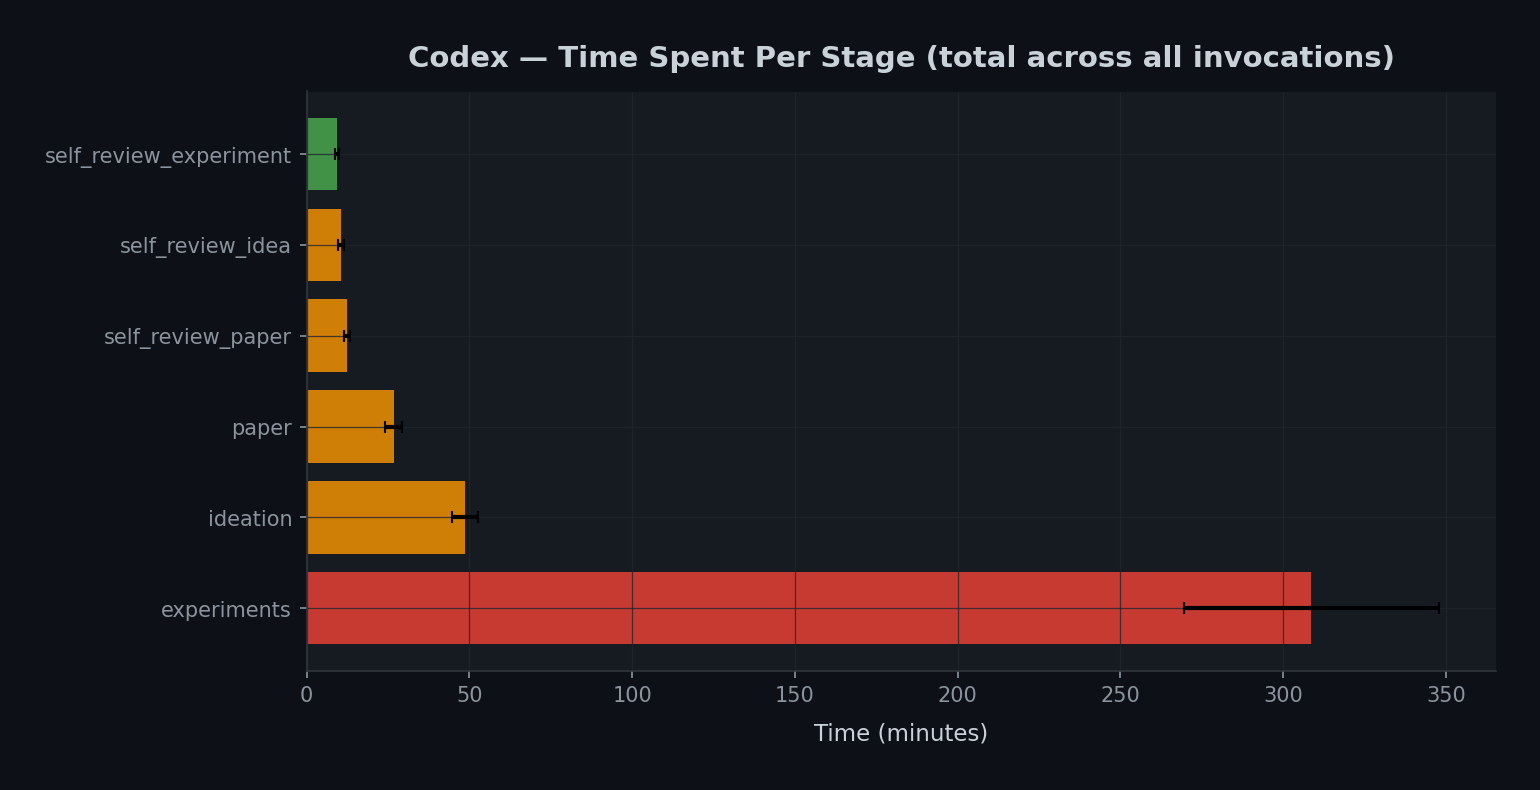
\includegraphics[width=\linewidth]{codex_time_per_stage.png}
\caption{Codex}
\end{subfigure}
\begin{subfigure}{0.32\linewidth}
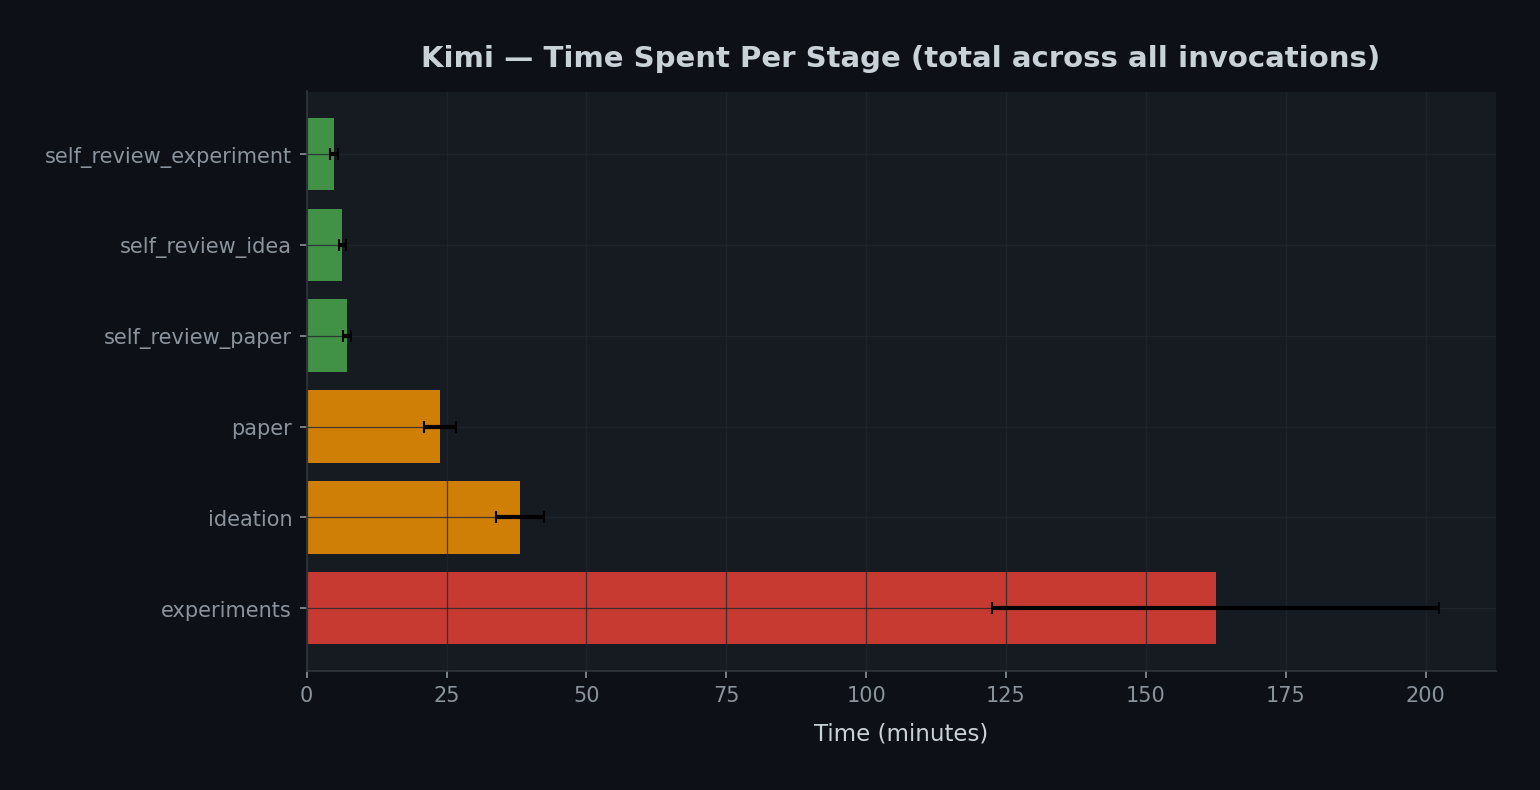
\includegraphics[width=\linewidth]{kimi_time_per_stage.png}
\caption{Kimi}
\end{subfigure}
\caption{Time per stage by agent.}
\end{figure}

\begin{figure}[h]
\centering
\begin{subfigure}{0.32\linewidth}
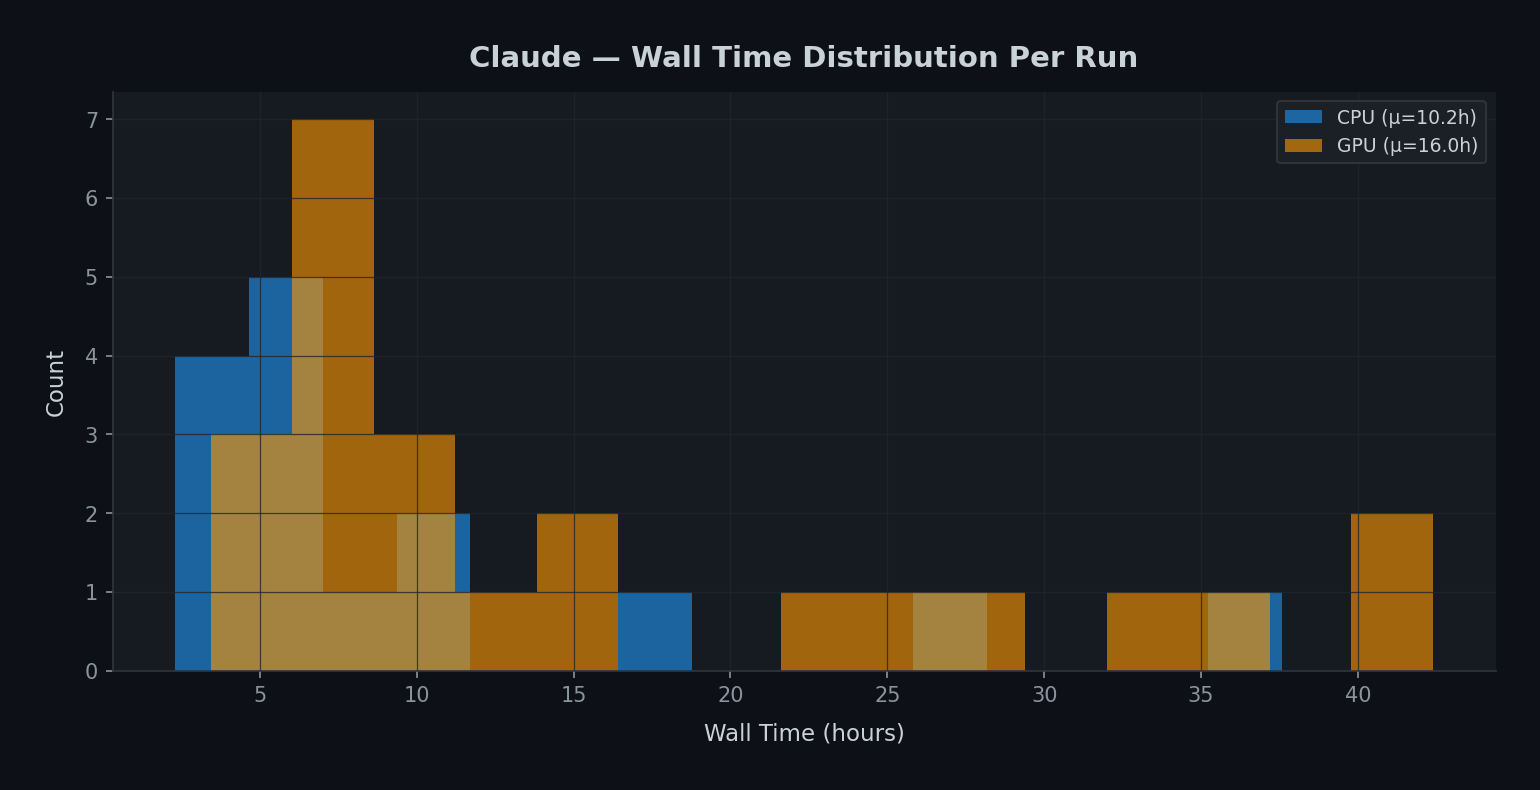
\includegraphics[width=\linewidth]{claude_wall_time.png}
\caption{Claude}
\end{subfigure}
\begin{subfigure}{0.32\linewidth}
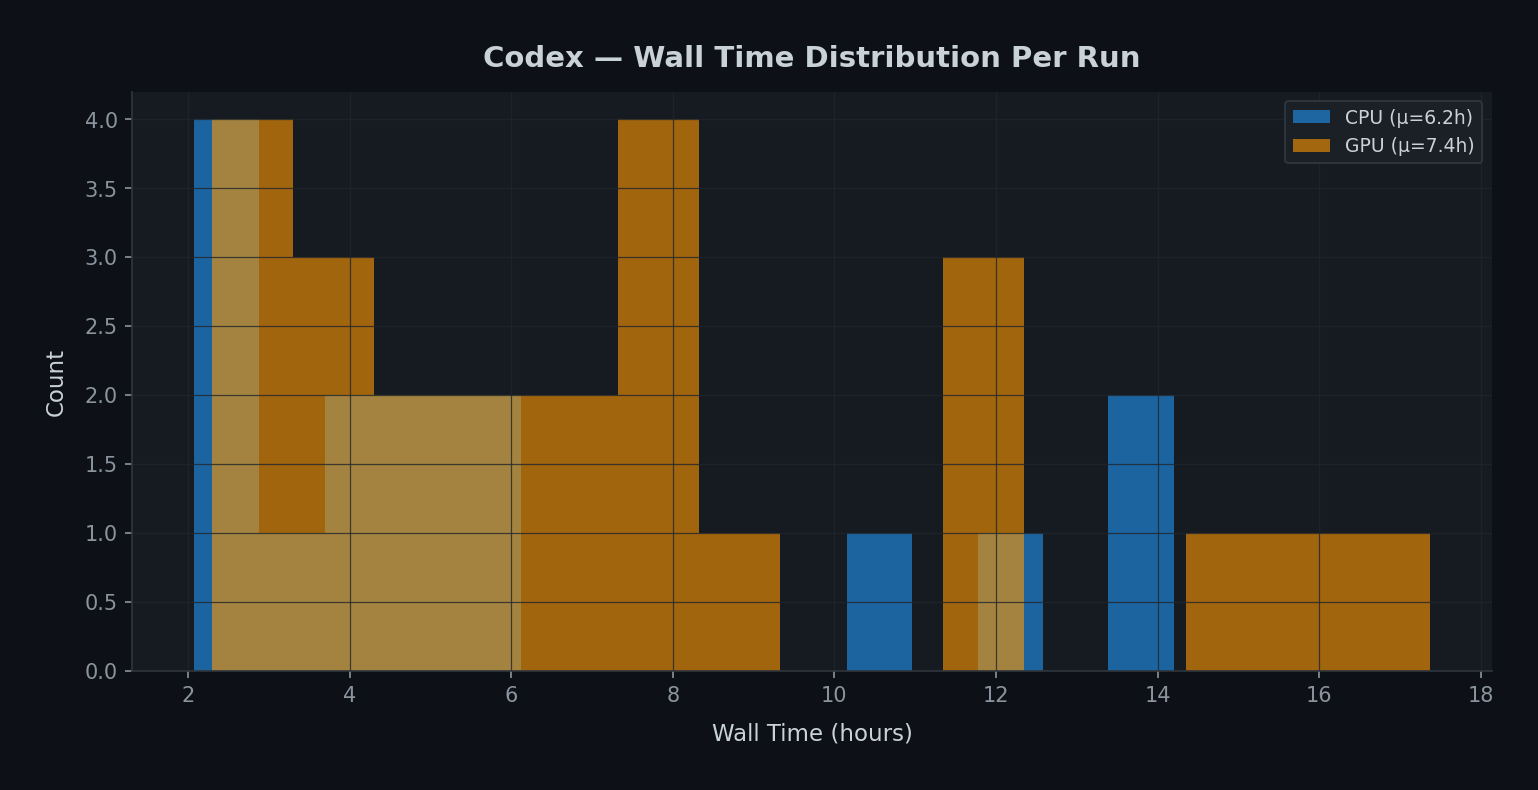
\includegraphics[width=\linewidth]{codex_wall_time.png}
\caption{Codex}
\end{subfigure}
\begin{subfigure}{0.32\linewidth}
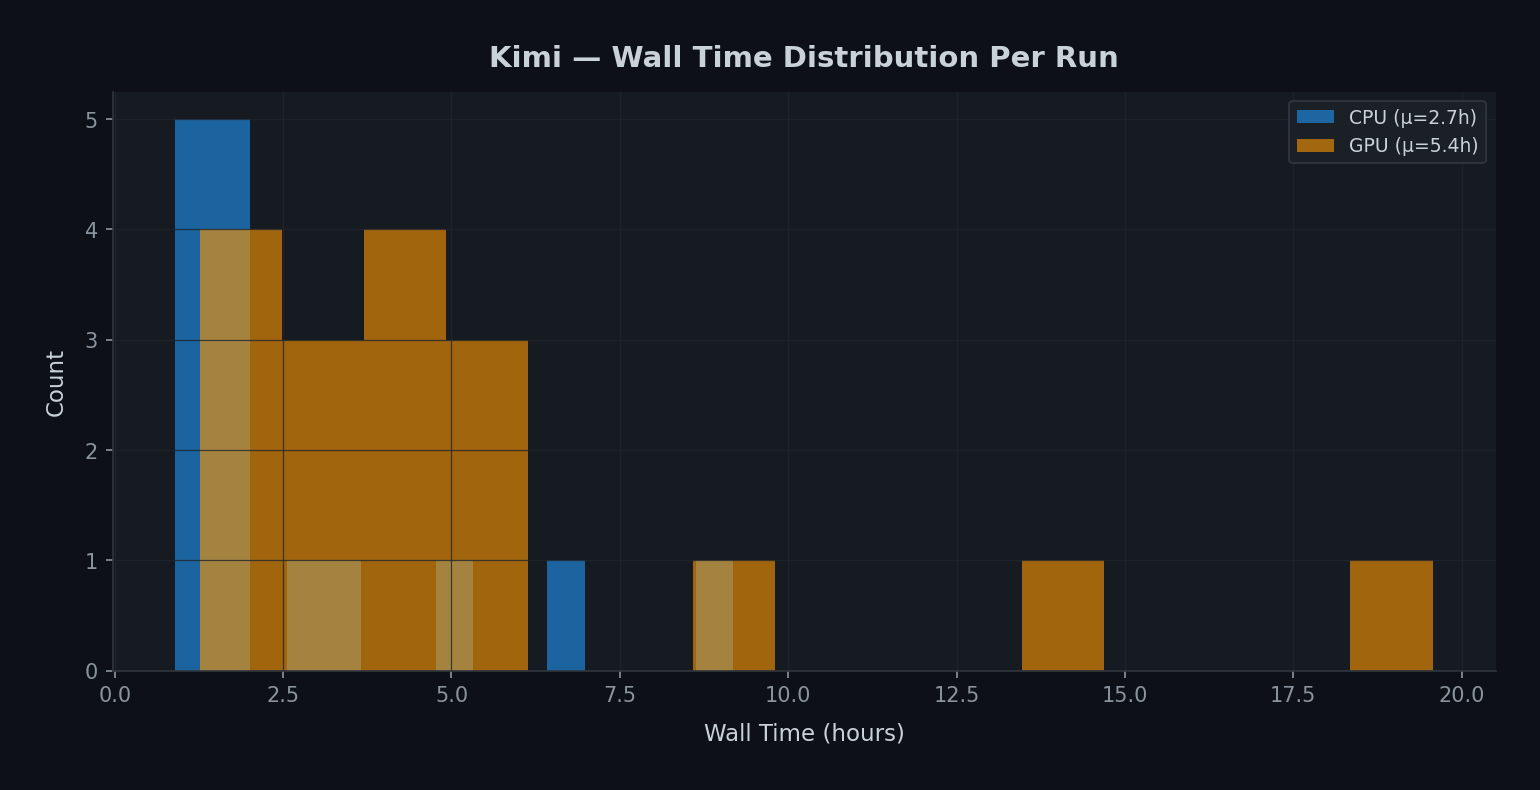
\includegraphics[width=\linewidth]{kimi_wall_time.png}
\caption{Kimi}
\end{subfigure}
\caption{Wall-time distributions by agent.}
\end{figure}

\begin{figure}[h]
\centering
\begin{subfigure}{0.32\linewidth}
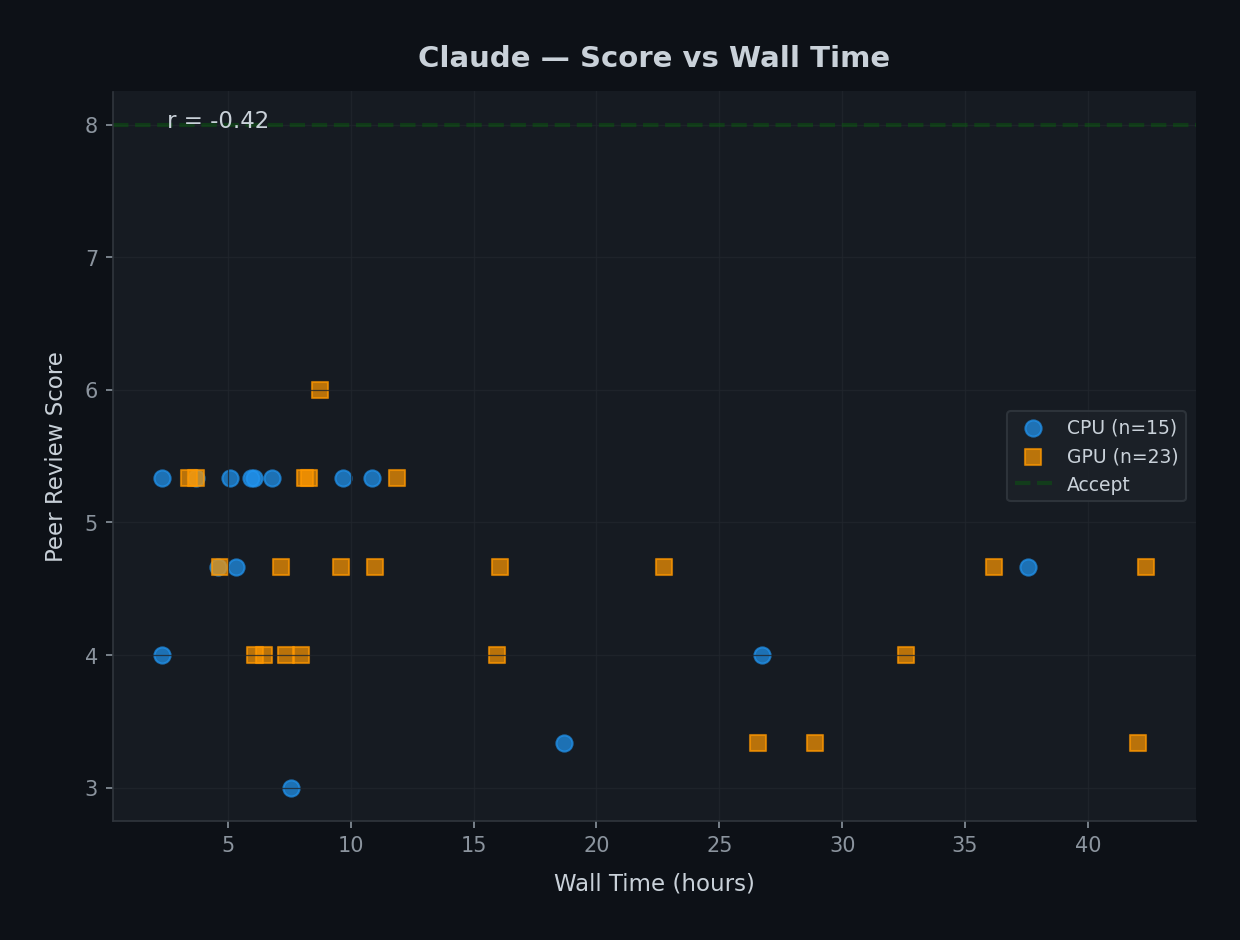
\includegraphics[width=\linewidth]{claude_score_vs_time.png}
\caption{Claude}
\end{subfigure}
\begin{subfigure}{0.32\linewidth}
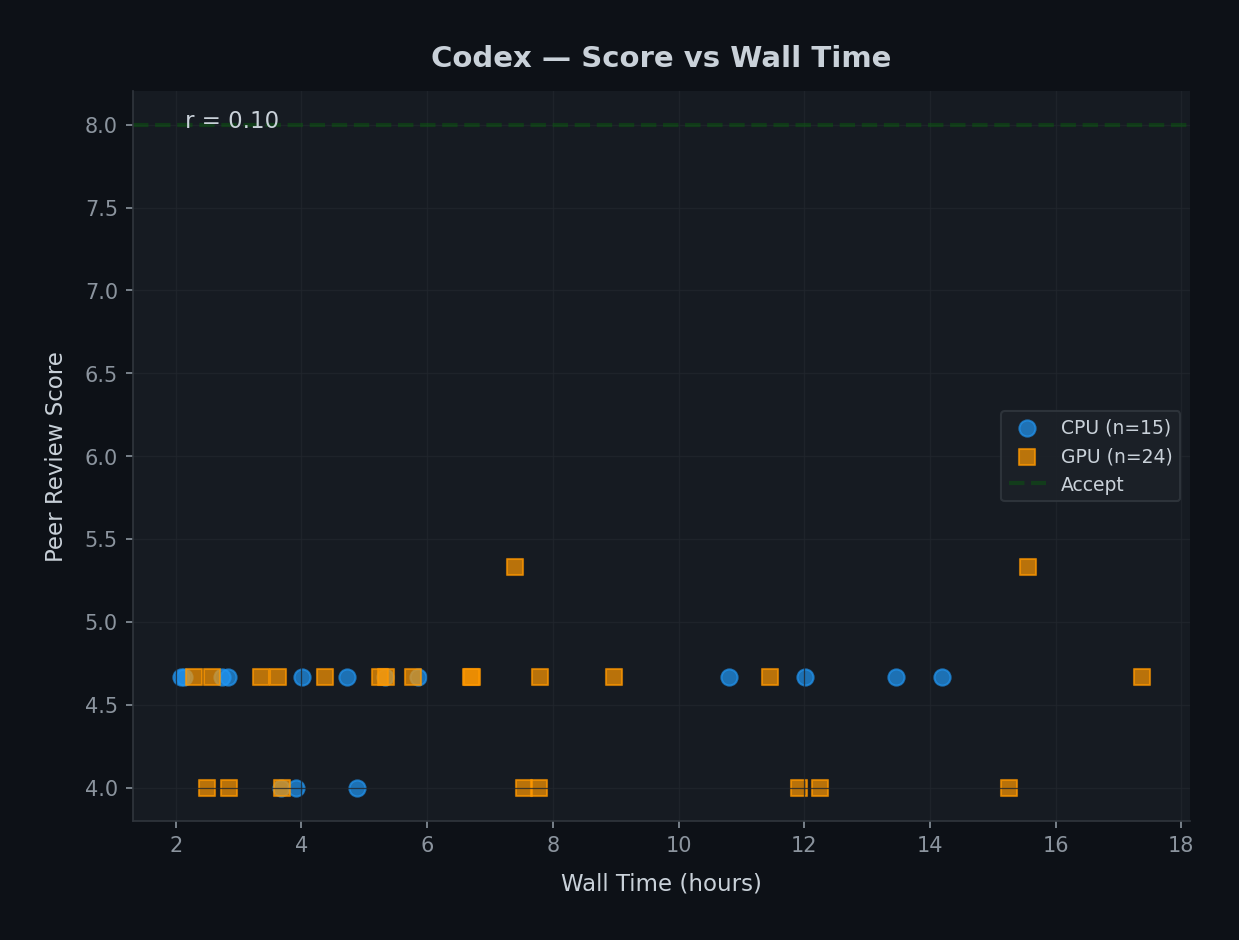
\includegraphics[width=\linewidth]{codex_score_vs_time.png}
\caption{Codex}
\end{subfigure}
\begin{subfigure}{0.32\linewidth}
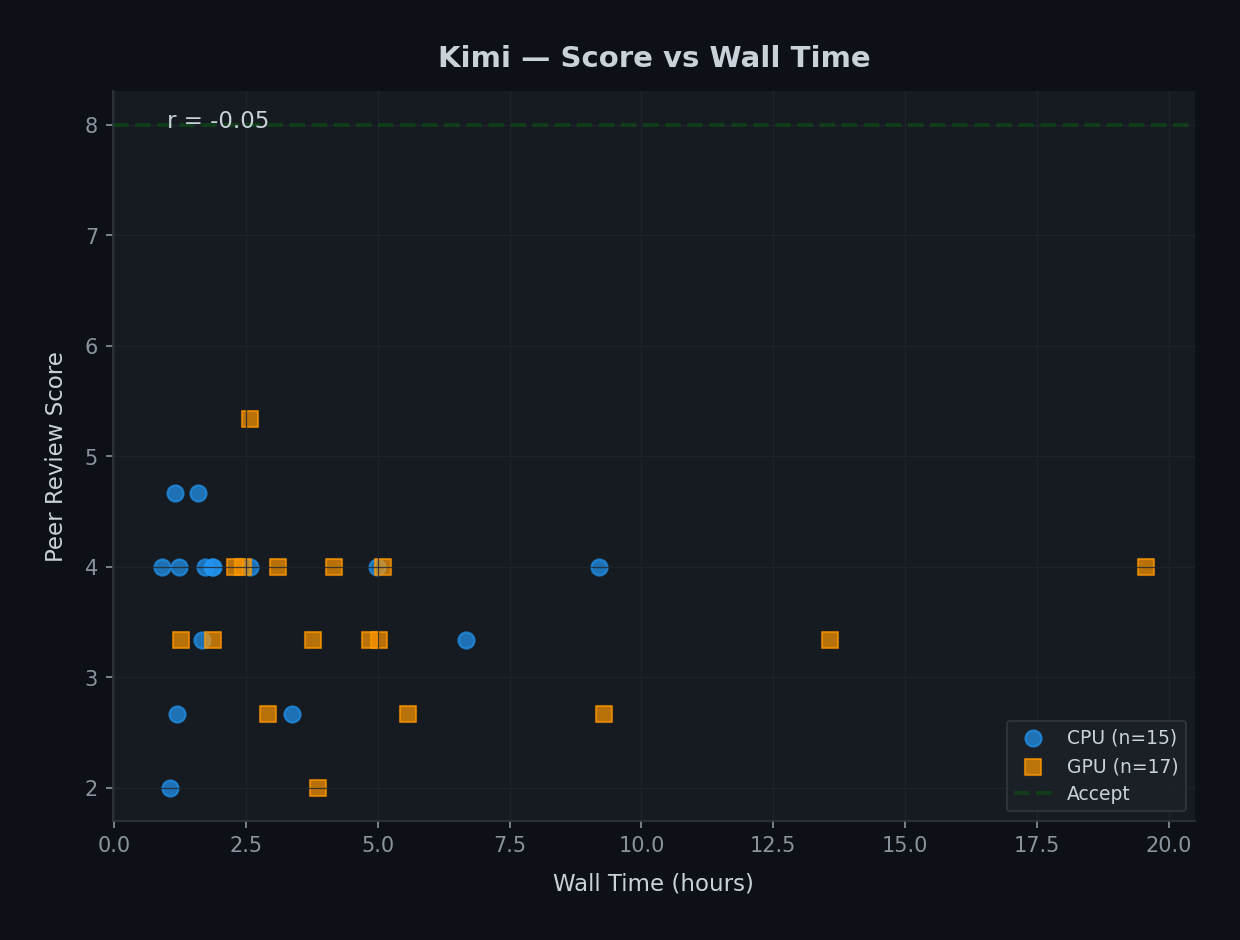
\includegraphics[width=\linewidth]{kimi_score_vs_time.png}
\caption{Kimi}
\end{subfigure}
\caption{Score versus time plots.}
\end{figure}

\begin{figure}[h]
\centering
\begin{subfigure}{0.32\linewidth}
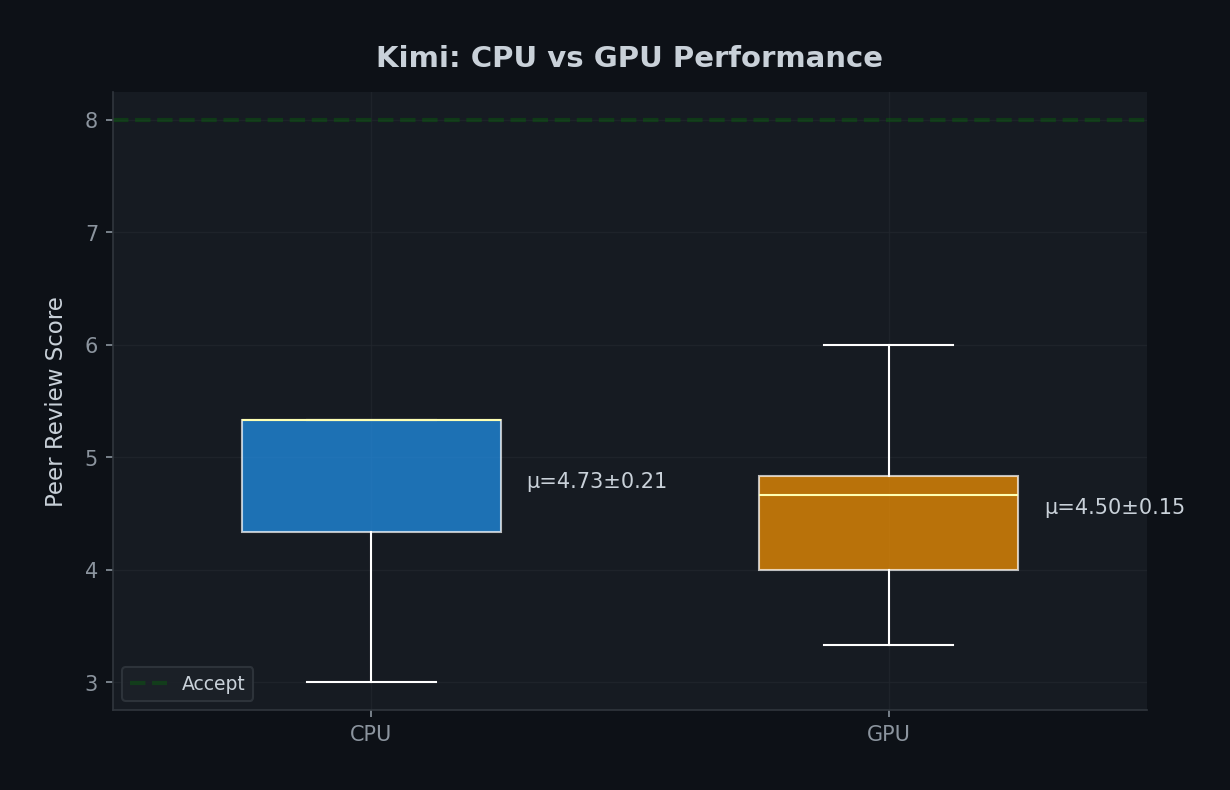
\includegraphics[width=\linewidth]{claude_cpu_vs_gpu.png}
\caption{Claude}
\end{subfigure}
\begin{subfigure}{0.32\linewidth}
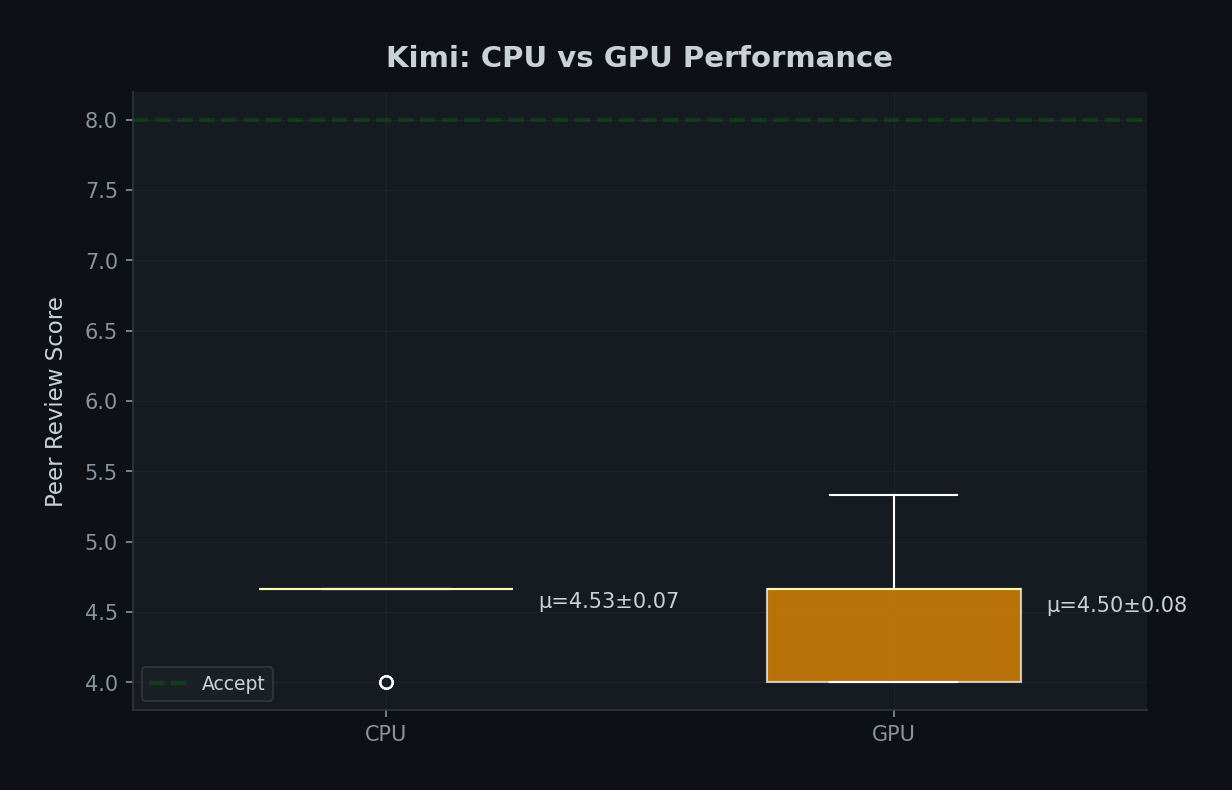
\includegraphics[width=\linewidth]{codex_cpu_vs_gpu.png}
\caption{Codex}
\end{subfigure}
\begin{subfigure}{0.32\linewidth}
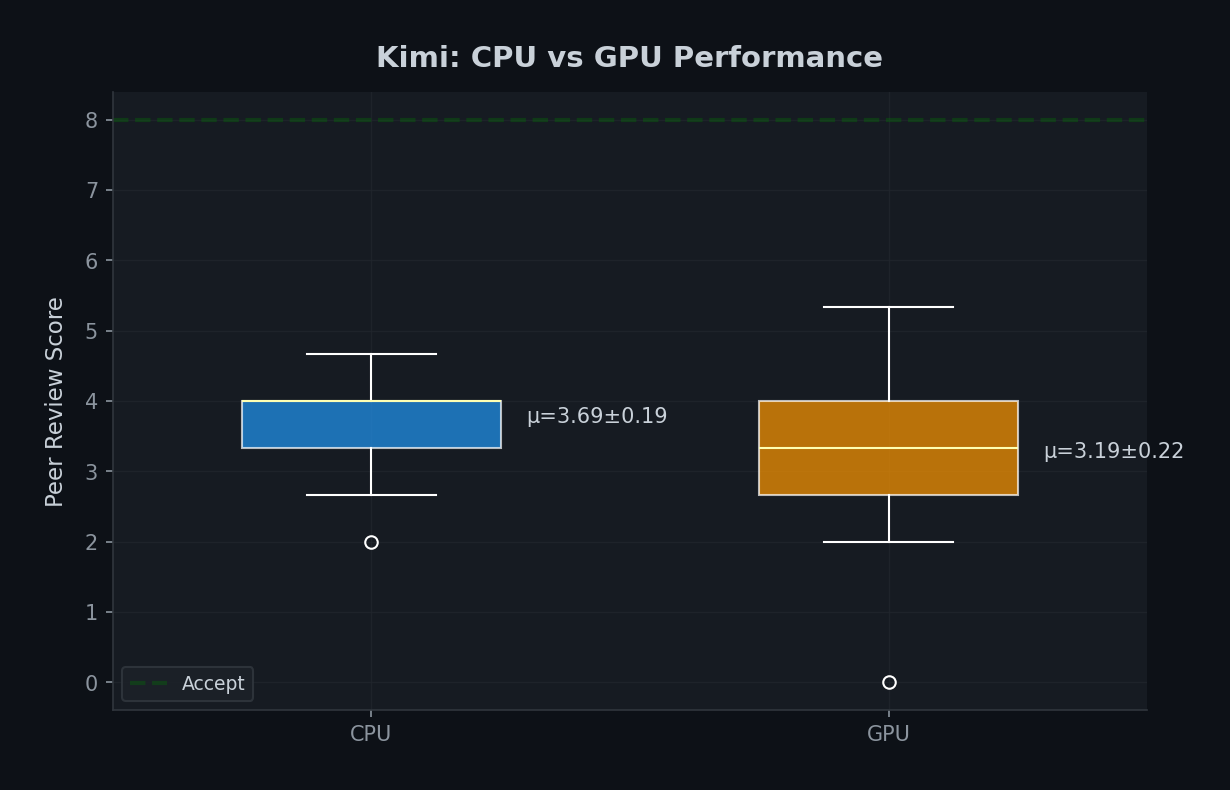
\includegraphics[width=\linewidth]{kimi_cpu_vs_gpu.png}
\caption{Kimi}
\end{subfigure}
\caption{CPU versus GPU diagnostics by agent.}
\end{figure}

\begin{figure}[h]
\centering
\begin{subfigure}{0.32\linewidth}
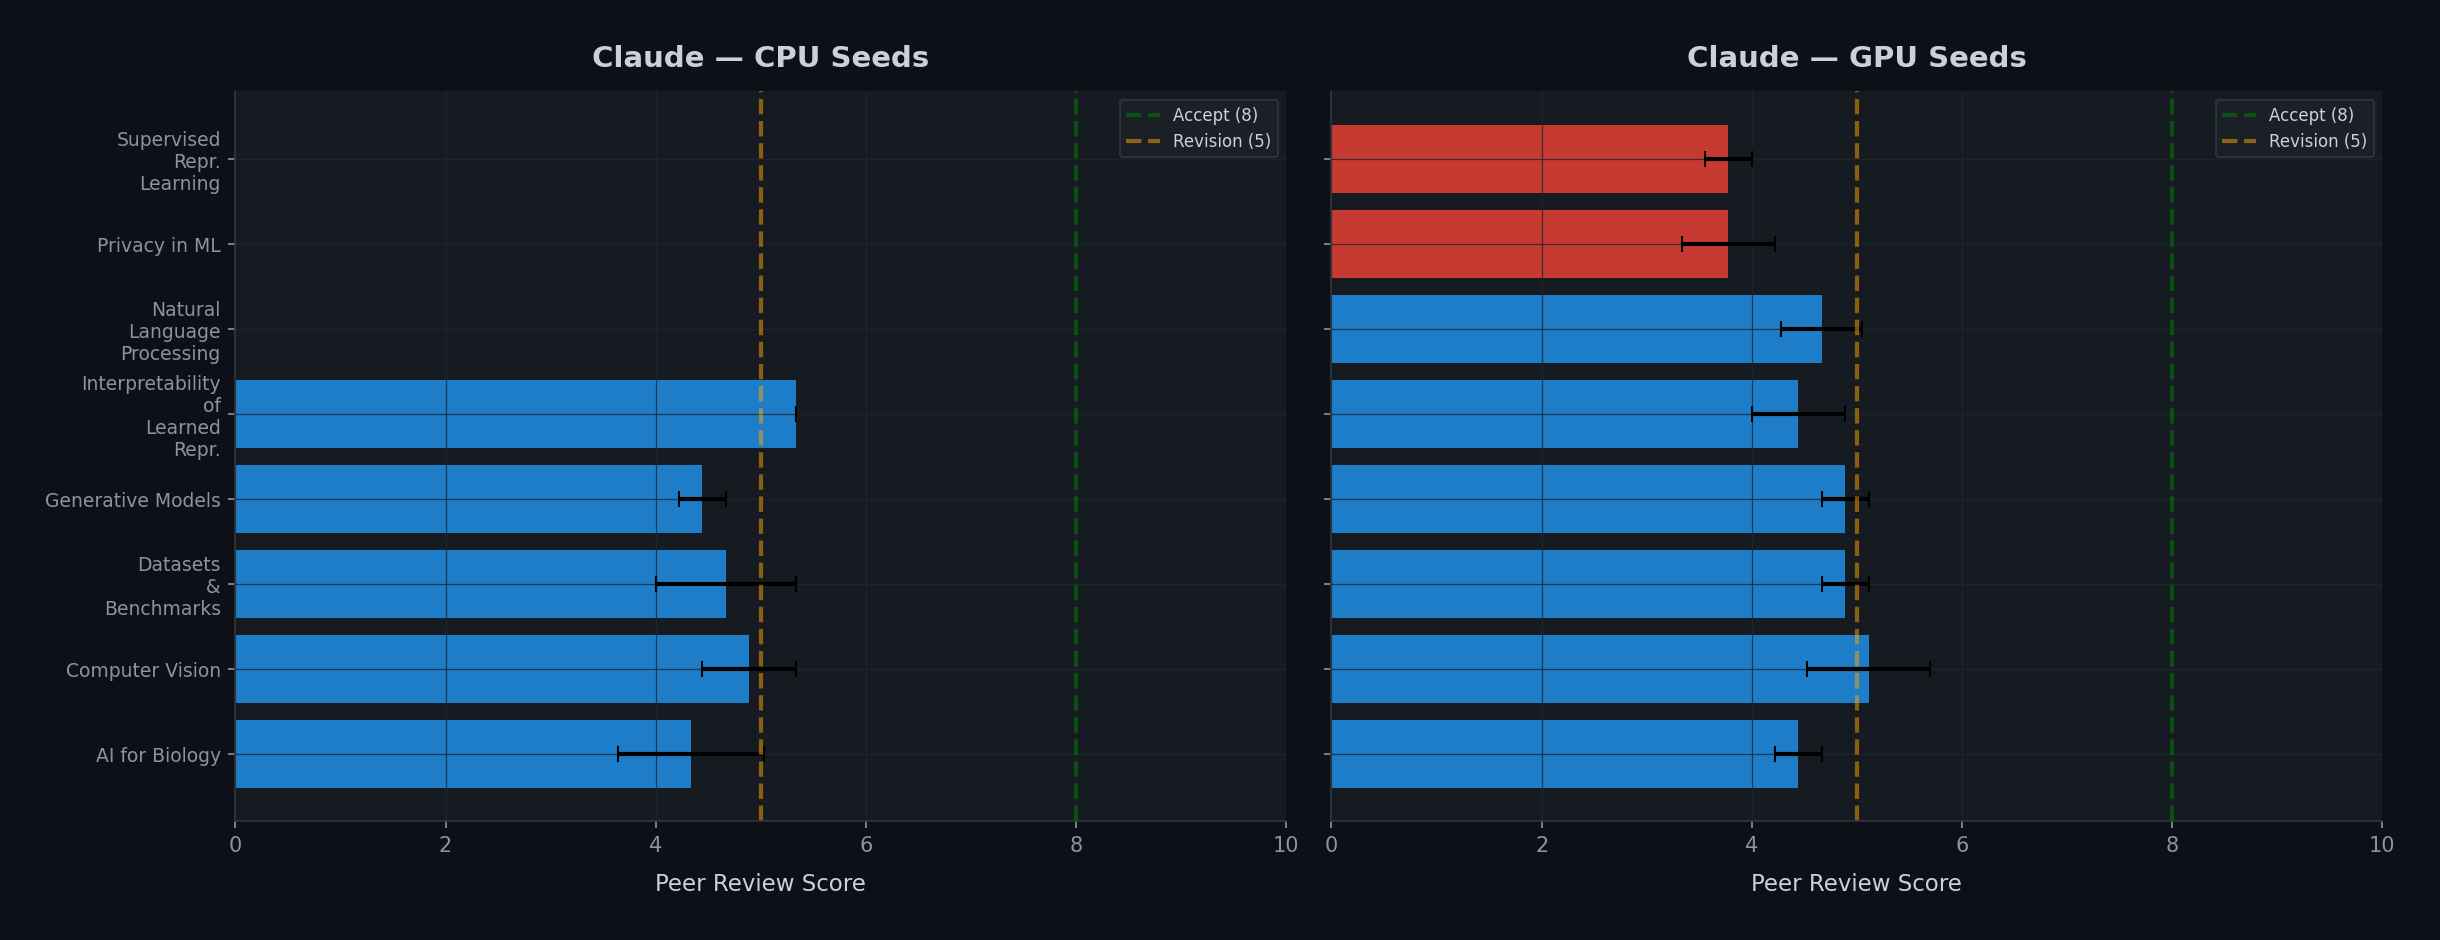
\includegraphics[width=\linewidth]{claude_scores_by_seed.png}
\caption{Claude}
\end{subfigure}
\begin{subfigure}{0.32\linewidth}
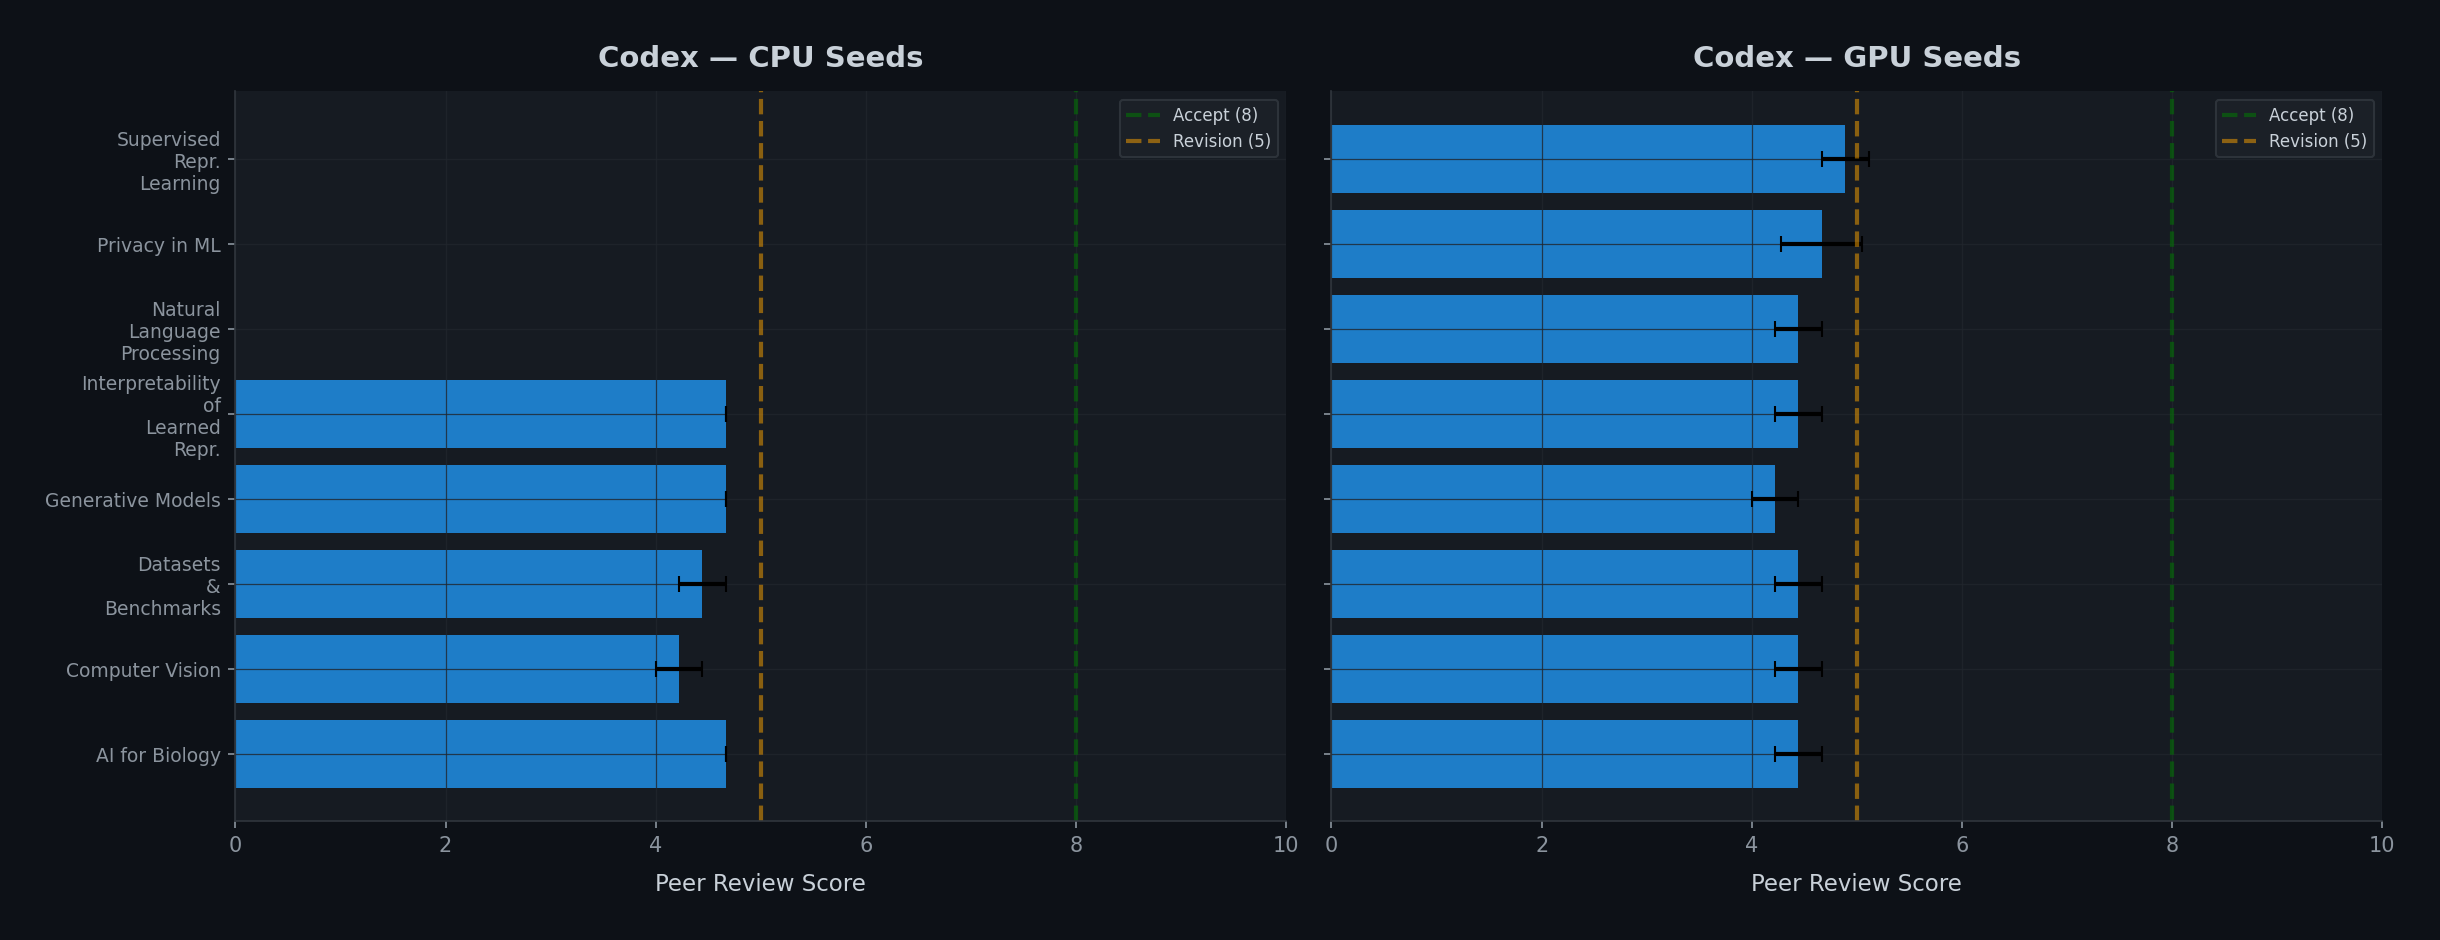
\includegraphics[width=\linewidth]{codex_scores_by_seed.png}
\caption{Codex}
\end{subfigure}
\begin{subfigure}{0.32\linewidth}
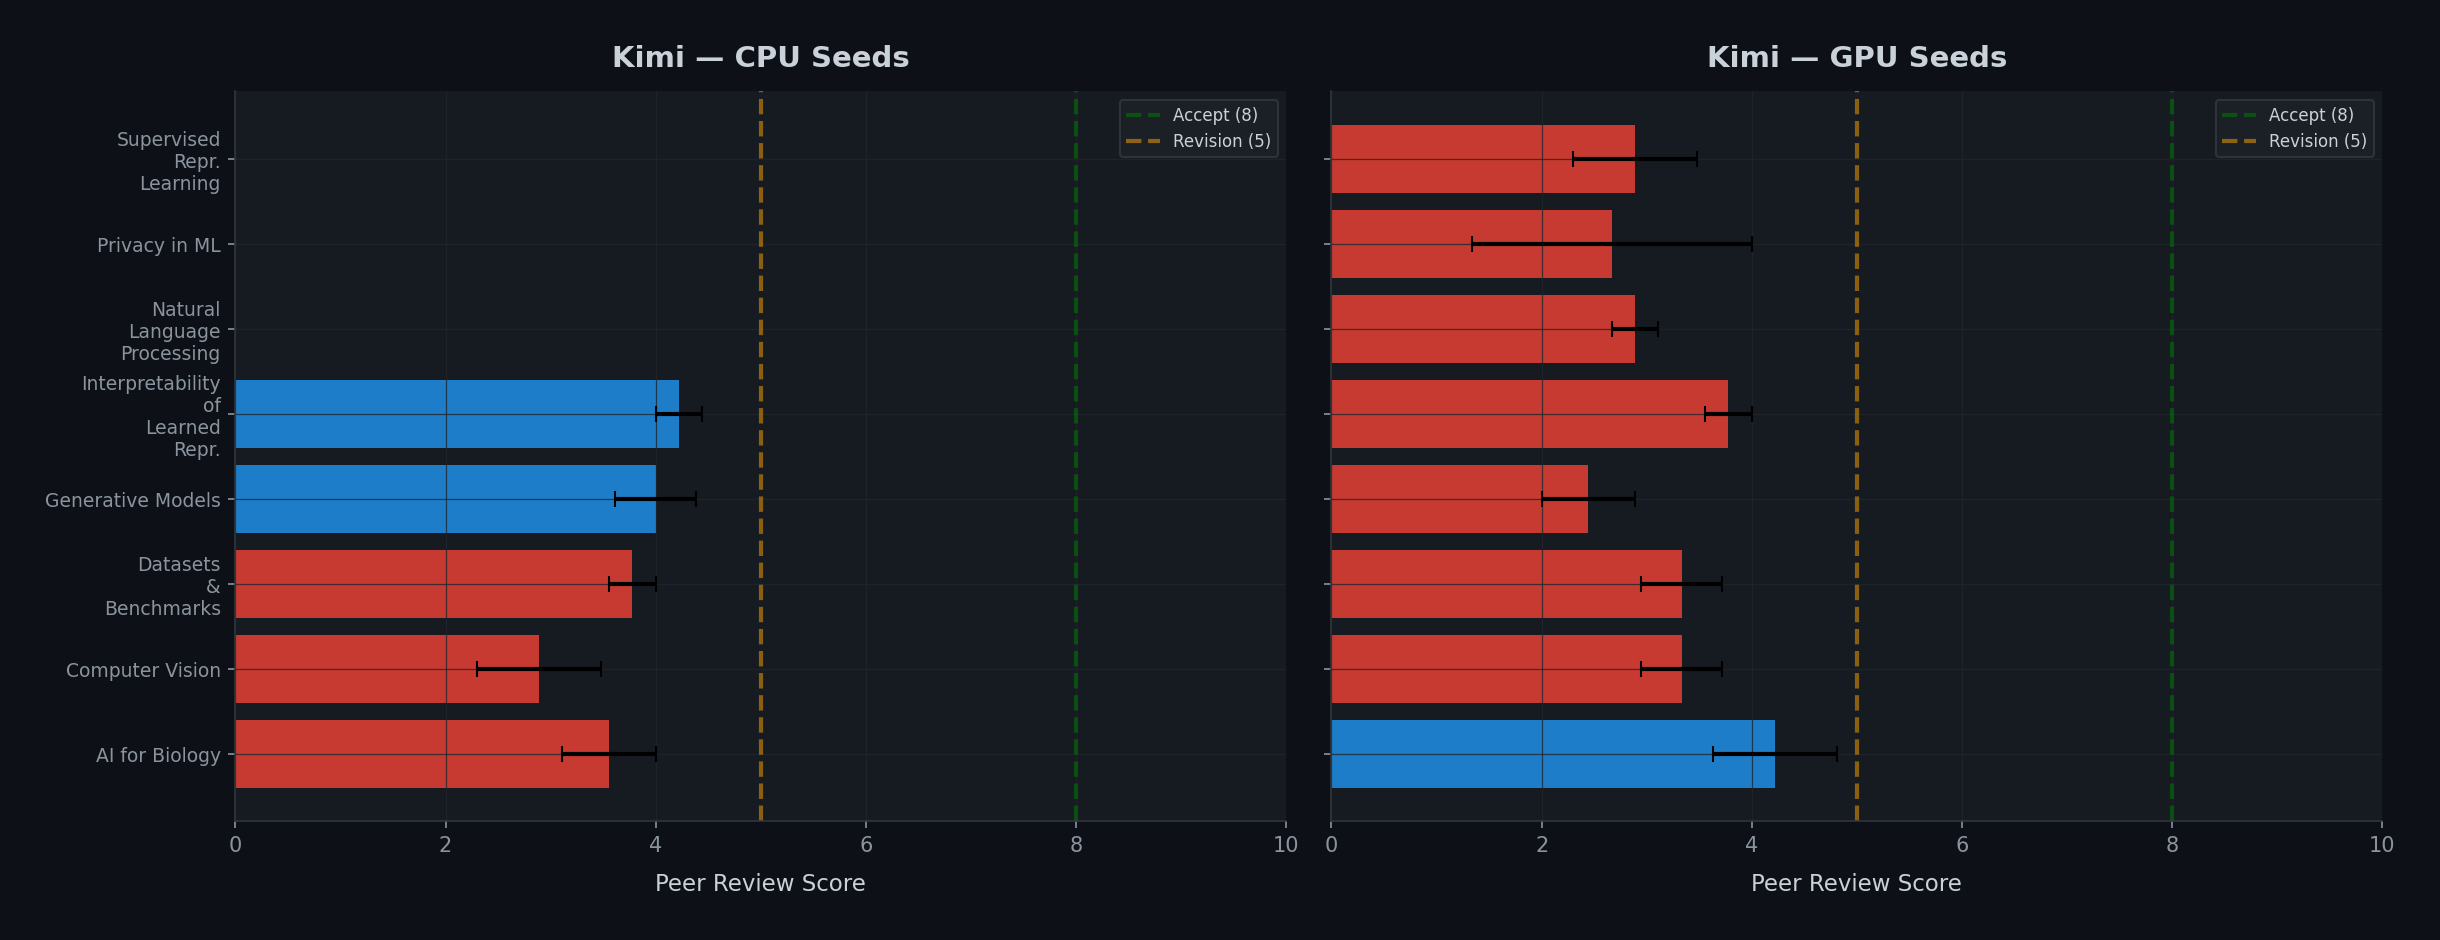
\includegraphics[width=\linewidth]{kimi_scores_by_seed.png}
\caption{Kimi}
\end{subfigure}
\caption{Scores by seed.}
\end{figure}

\begin{figure}[h]
\centering
\begin{subfigure}{0.32\linewidth}
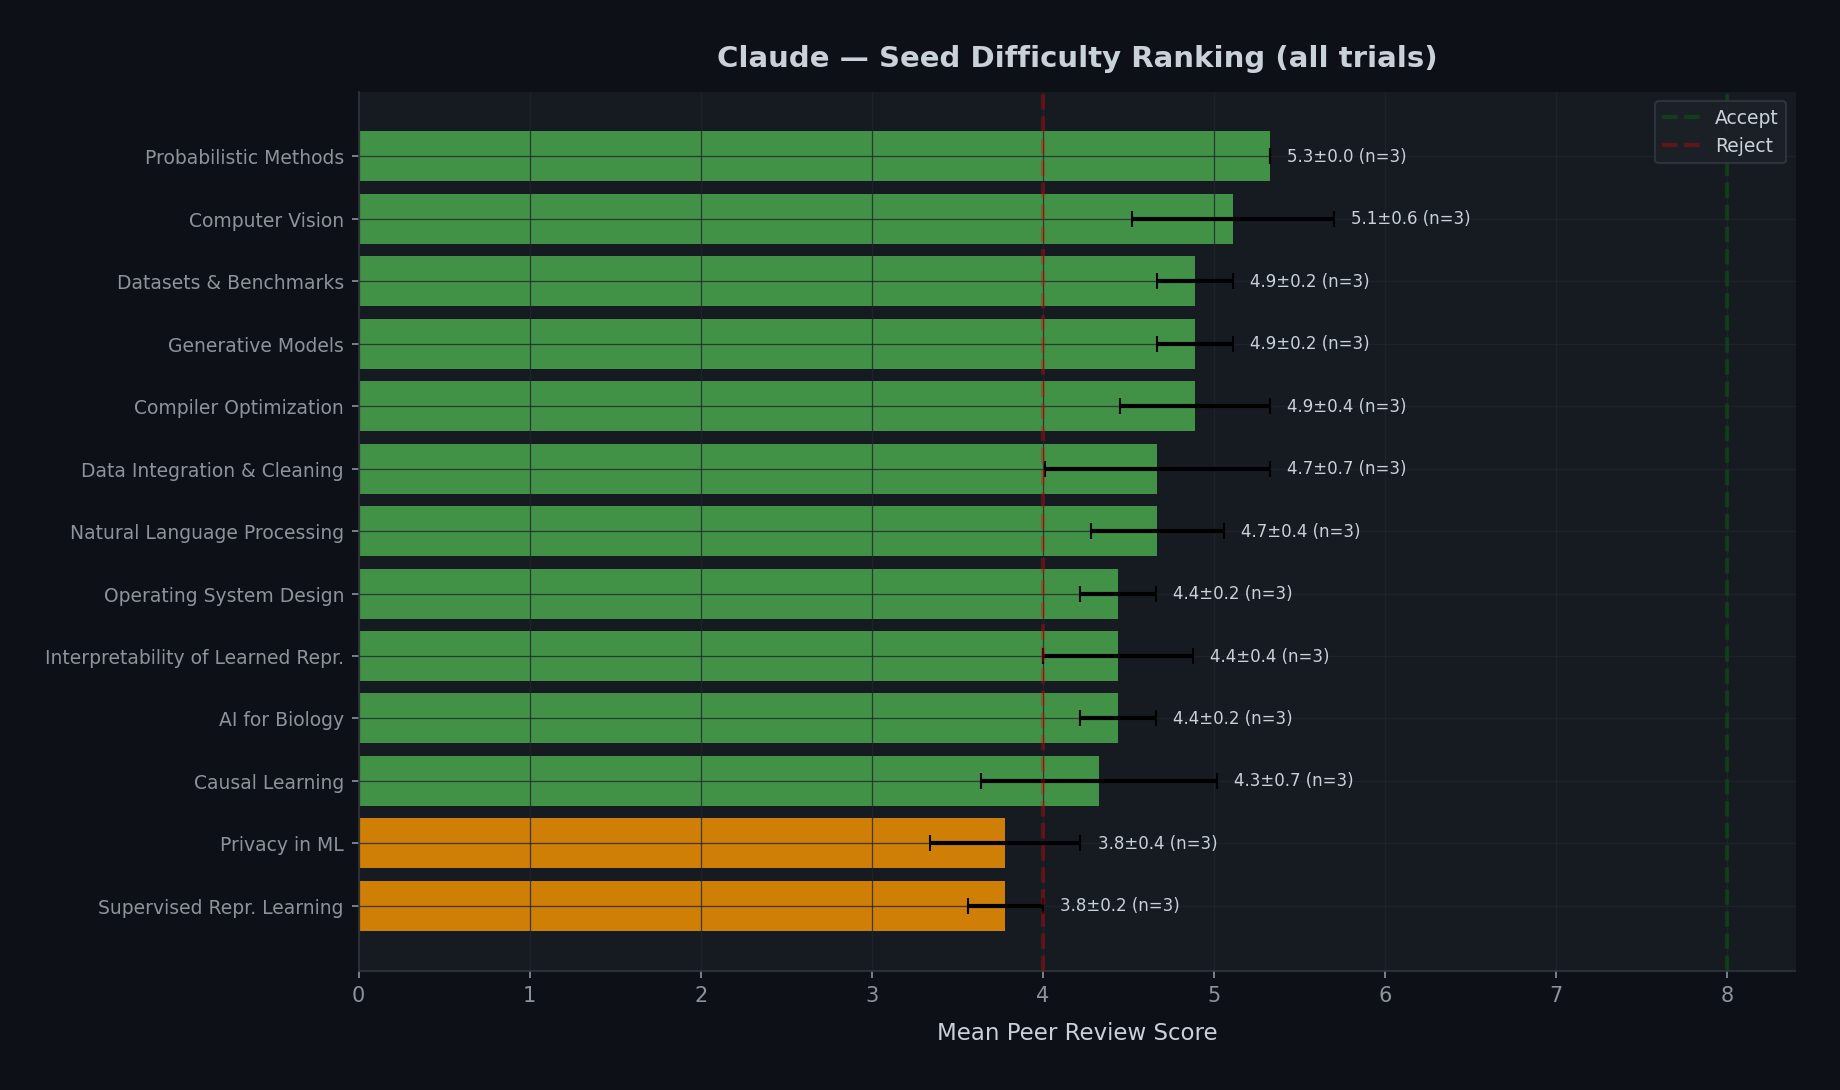
\includegraphics[width=\linewidth]{claude_seed_difficulty.png}
\caption{Claude}
\end{subfigure}
\begin{subfigure}{0.32\linewidth}
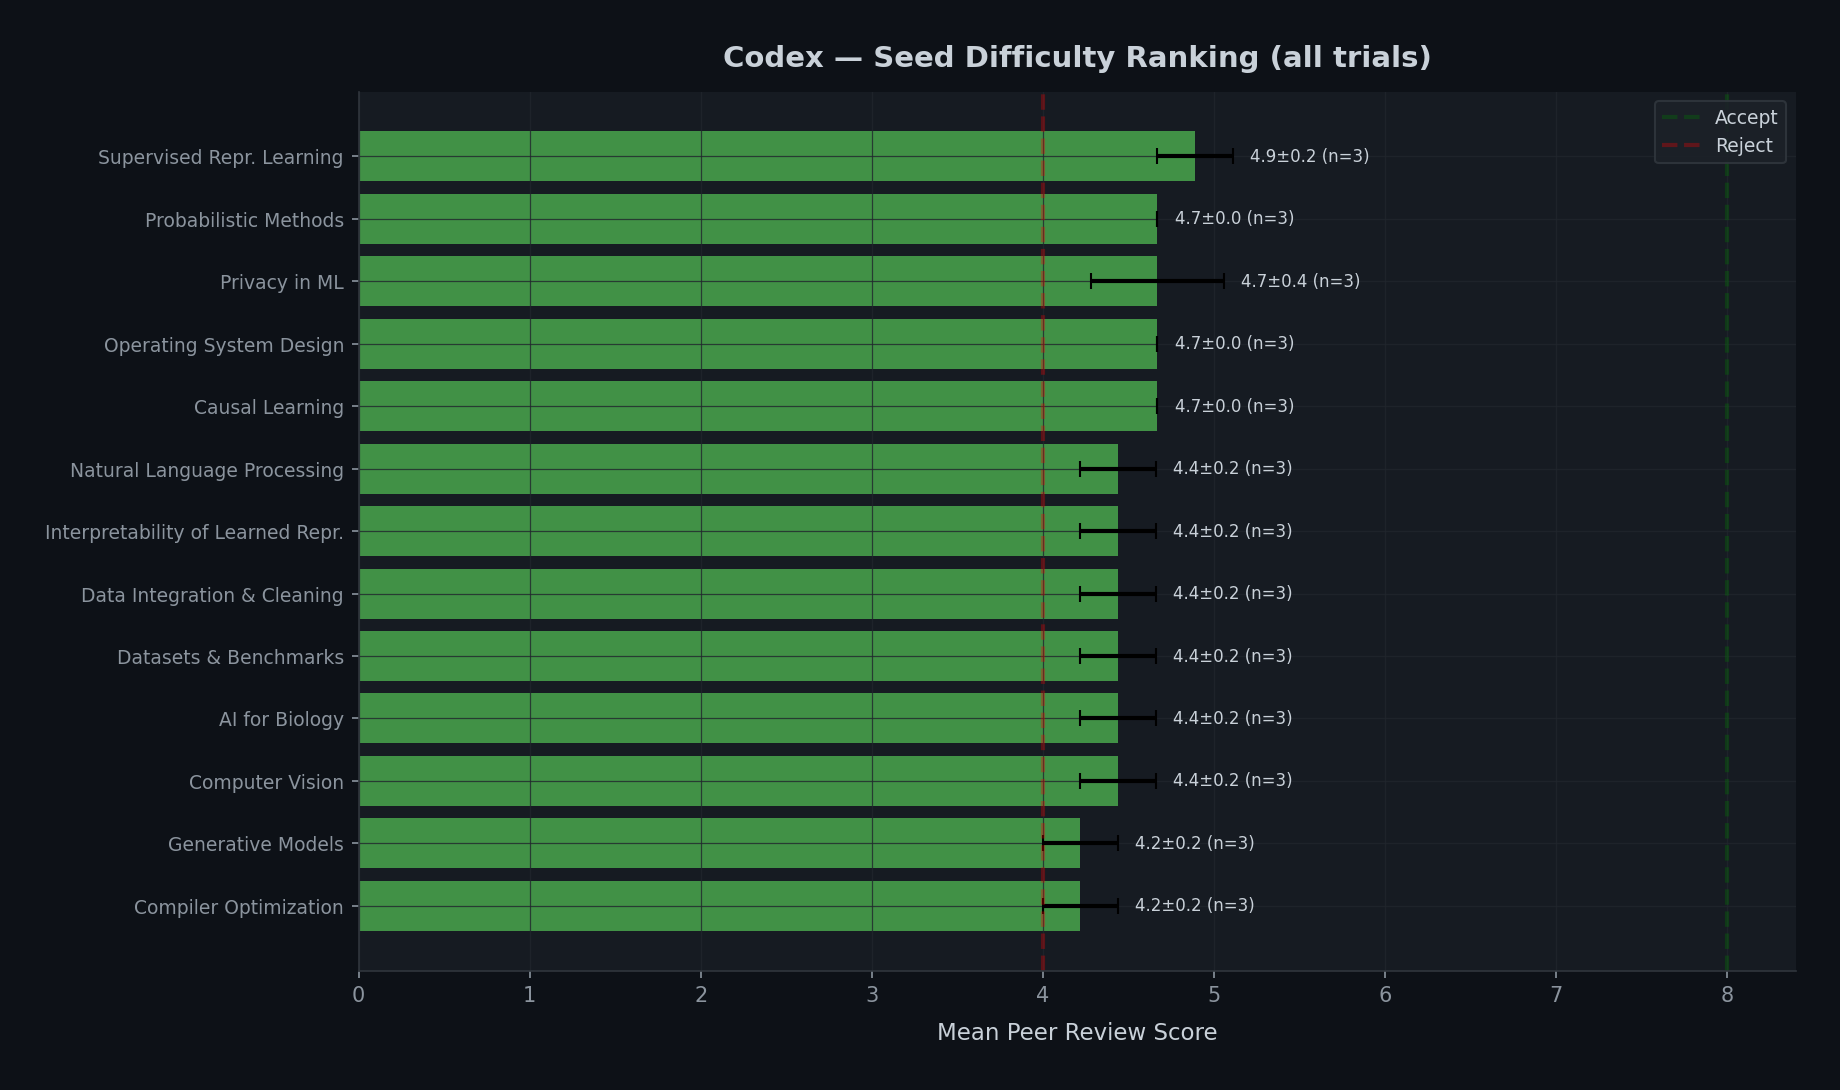
\includegraphics[width=\linewidth]{codex_seed_difficulty.png}
\caption{Codex}
\end{subfigure}
\begin{subfigure}{0.32\linewidth}
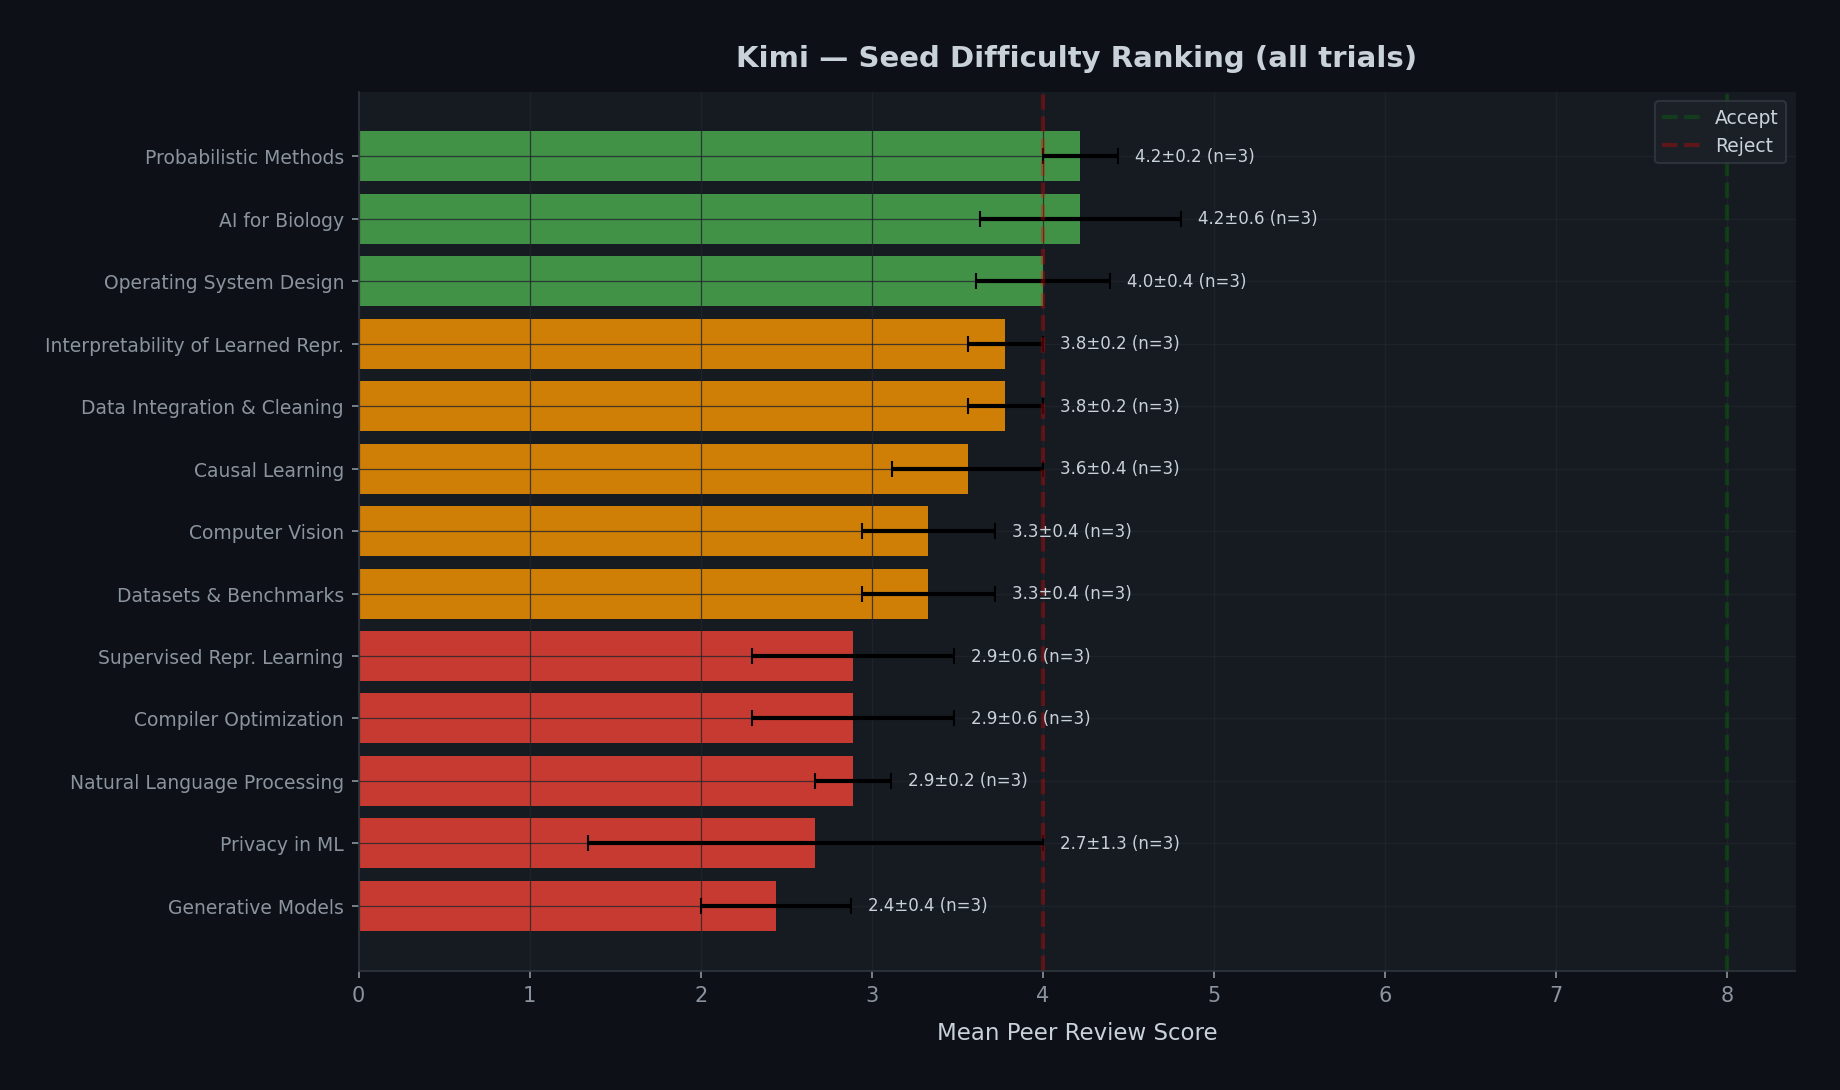
\includegraphics[width=\linewidth]{kimi_seed_difficulty.png}
\caption{Kimi}
\end{subfigure}
\caption{Seed difficulty diagnostics.}
\end{figure}

\begin{figure}[h]
\centering
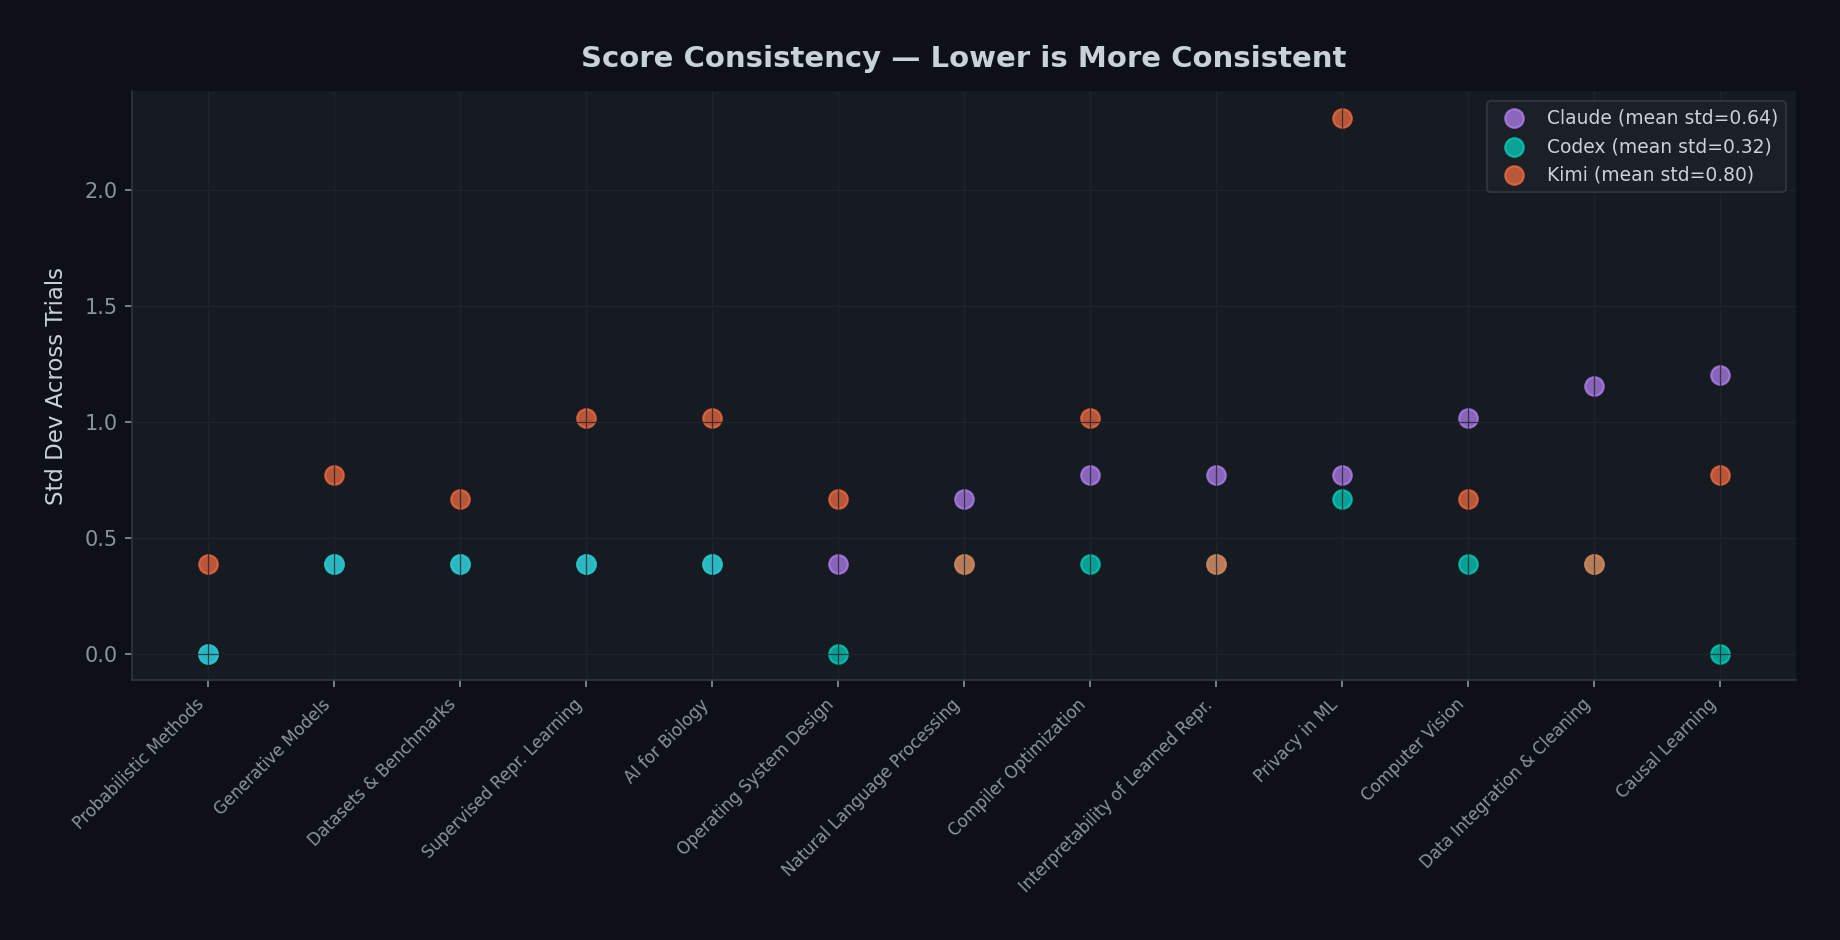
\includegraphics[width=0.75\linewidth]{comparison_3way_consistency.png}
\caption{Consistency comparison across the three agents.}
\end{figure}

\subsection{Paper Structure}

\begin{table}[h]
\centering
\small
\begin{tabular}{lrrr}
\toprule
Metric & Claude Code & Codex & Kimi Code \\
\midrule
Paper length (words) & 4023 & 3421 & 2461 \\
Method section (words) & 572 & 531 & 394 \\
Equations & 3.8 & 2.3 & 4.0 \\
Figures & 4.8 & 4.1 & 0.8 \\
Tables & 6.0 & 4.2 & 4.0 \\
Algorithm blocks & 0.6 & 0.0 & 0.6 \\
Theorems/proofs & 0.3 & 0.0 & 0.4 \\
Complexity analysis & 77\% & 10\% & 64\% \\
\bottomrule
\end{tabular}
\caption{Paper-structure metrics across the 39 papers per agent.}
\end{table}

\begin{table}[h]
\centering
\small
\begin{tabular}{lrrr}
\toprule
Title metric & Claude Code & Codex & Kimi Code \\
\midrule
Average title length & 102 chars & 99 chars & 92 chars \\
Question titles & 10\% & 28\% & 0\% \\
Colon structure & 74\% & 46\% & 85\% \\
Contains acronym & 15\% & 49\% & 51\% \\
Named method starts title & 21\% & 38\% & 46\% \\
\bottomrule
\end{tabular}
\caption{Title-style metrics.}
\end{table}


\end{document}
